% Aquí contendrán los métodos y procedimientos adoptados en el desarrollo del trabajo. Esta es una de las sesiones más importantes pues demuestra el poder científico que se utilizó para la investigación. Sin una buena metodología la investigación puede perder la validez. El investigador debe utilizar métodos o técnicas aceptadas por la comunidad científica en la búsqueda de probar sus hipótesis.

% La metodología elegida debe ser aquella que más se adecue a su objeto de estudio y al enfoque aplicado. Hay dos métodos principales: 1) cuantitativo, que es el uso de instrumental estadístico, de datos numéricos; y 2) cualitativo, que se caracteriza por la calificación de los datos recogidos, durante el análisis del problema.

% ENLACES VISTOS
% COURSERA: La Web Semántica: Herramientas para la publicación y extracción efectiva de información en la Web
% CURSO EN COURSERA INTERESANTE: https://es.coursera.org/learn/web-semantica?action=enroll
% http://www.fgcsic.es/lychnos/es_es/articulos/construyendo_una_web_semantica
% Libro Geospatial Semantic Web
% https://www.researchgate.net/publication/216537707_La_Web_semantica_y_las_tecnologias_del_lenguaje_humano
% http://www.bibliopos.es/Biblion-A2-Bibliografia-Documentacion/18ontologia-Web-Semantica.pdf

\chapter{Web Semántica}
\label{ch:web-semantinca}

\begin{quote}
  {\bf\textsc{Resumen:}} 
\end{quote}

\section{Conceptos Generales}


A continuación, vamos a introducir la definición de Web Semántica, para ello se va a realizar previamente un pequeño estudio del arte sobre la evolución de la Web hasta lo que conocemos actualmente.

\subsection{Conceptos generales de la Web}

%% ANTECEDENTES

% https://disenowebakus.net/semantica-web.php
La revolución informática, acaecida durante el siglo XX, llevó consigo la introducción de cambios severos en diversos aspectos de la sociedad. De entre todas estas transformaciones, fueron muchos los que vaticinaron un nuevo mundo, fundamentado principalmente por la aparición de la informática personal, en donde los seres humanos tendrían acceso a grandes repositorios de información. Este nuevo concepto trajo consigo lo que actualmente conocemos como \textit{búsqueda y consulta de información}, en donde los usuarios únicamente podían acceder a dicha información mediante rutas de acceso delimitadas por los diseñadores del sistema. Aunque la información podía ser localizada de diversas maneras (formularios, clasificaciones...), era un escenario en donde las consultas a las bases de datos en línea estaban reservadas a usuarios muy específicos (generalmente investigadores) y casi siempre a través de un intermediario, un documentalista. Por supuesto la búsqueda de información se realizaba sobre información textual, generalmente sin estructura e incluso sin formato. Gracias a la introducción de Internet en todos los ámbitos de nuestra sociedad, más allá del uso científico o académico, sólo fue cuestión de tiempo y revolucionó el panorama anteriormente descrito.

%% DEFINICIÓN DE WEB, CUANDO SE CREO, QUIEN LA CREO, COMO SURGIÓ

% https://disenowebakus.net/semantica-web.php
Como consecuencia, la Web se ha convertido en un instrumento de uso cotidiano para el intercambio de información en nuestra sociedad, llegando a superar a medios como la televisión, y se ha constituido, junto con el papel, en uno de los medios de publicación más importante en la sociedad actual. Por tanto, la Web actual, ha evolucionado hacia usos que han trascendido la idea original de Tim Berners-Lee.

% AVANCE WEB

% https://disenowebakus.net/semantica-web.php
Ya no estamos hablando de un sistema para publicar y comunicar resultados de experimentos y trabajos de investigación. Sobre aquella Web, se basada en la interconexión de documentos mediante enlaces de hipertexto, se han creado nuevas herramientas gracias al desarrollo de lenguajes de programación para la Web y su integración con sistemas de base de datos. El concepto de Sistema de Gestión de Contenidos plantea la Web como una plataforma universal para la creación de todo tipo de herramientas, cuyo uso únicamente precisa del usuario un sólo software esencial: el navegador Web. Los usuarios comenzaron a interactuar con la Web más allá de la búsqueda y consulta de información.

% FUNCIONALIDAD WEB ACTUAL

% COURSERA: La Web Semántica: Herramientas para la publicación y extracción efectiva de información en la Web
¿Y cómo es la web actual? Primero la web actual es masiva. ¿Cuántos millones y millones de páginas web existen? Además la web actual es cambiante ¿Cuántos tweets por segundo se generan? ¿Cuántas actualizaciones de perfil de Facebook se generan? Incontables, además la web actual es heterogénea ¿Cuántos millones de dispositivos como éste, o como sensores generan datos? La web actual además es distribuida, cualquier persona en el mundo puede acceder o generar contenido, no solo esto la web actual es un gran repositorio de información al cual todo el mundo puede acceder.

% https://disenowebakus.net/semantica-web.php
Las funcionalidades de creación de contenidos textuales y audiovisuales y la comunicación entre individuos y grupos cristalizó en una nueva generación de herramientas conocida como Web 2.0 o Web social, orientadas a facilitar la conexión entre las personas. El factor humano dejó de ser un elemento pasivo para convertirse en una agente activo en la Web. La idea fundamental se centra en el establecimiento de redes o comunidades de usuarios que trabajan con una serie de servicios basados en aplicaciones Web como los blogs, los servicios de publicación de contenidos multimedia, las redes sociales o las wikis. Se trata de un uso concreto de la Web, que fomenta la colaboración para difundir e intercambiar información de forma rápida y sencilla. Sin embargo, hemos de tener en cuenta que esta situación implica una serie de problemas derivados de la propia naturaleza de una Web en la que participan los usuarios. Existen cantidades enormes de recursos desorganizados, duplicados o desactualizados, entre los que encontrar la información buscada termina resultando un trabajo arduo. Los motores de búsqueda Web, aunque han mejorado en los últimos años, continúan catalogando sólo una porción pequeña de la Web y a veces producen resultados que no son pertinentes y a menudo inexactos o imposibles de encontrar. Esto se debe a que la cantidad, estructura y originalidad de contenidos en la Web no han evolucionado paralelamente a como lo han hecho los procesos de publicación de los mismos. Existen gran cantidad de páginas duplicadas, puesto que muchos usuarios prefieren copiar contenidos en vez de referenciarlos con enlaces de hipertexto. Multitud de páginas hacen un uso incorrecto de metadados HTML, distorsionando su utilidad en los procesos de búsqueda. Tampoco es posible distinguir en todos los casos el tipo de recurso recuperado durante la búsqueda: un documento informativo, una ficha de una aplicación en un servicio de descarga de pago, una entrada en un foro de debate, etc. En este contexto, los buscadores Web son incapaces en ocasiones de ofrecer unos resultados útiles. 

% USO METADATOS 
% INTRODUCIR AL FINAL LA WEB SEMÁNTICA (VER COMO HACERLO) Y ASÍ UNIRLO AL SIGUIENTE APARTADO

% COURSERA: La Web Semántica: Herramientas para la publicación y extracción efectiva de información en la Web
¿Pero es realmente accesible esta información? Hoy en idea tenemos herramientas como Google y Bing y muchas otras que nos dan acceso a los datos. Pero estas herramientas tienen dificultades al momento de entender la información que está contenida en ellos. En particular estas herramientas miran las páginas web como si fueran conjunto de palabras, y no son capaces de entender o tienen dificultades al momento de entender los distintos elementos que forman parte de ella, que pueden ser tan diversos como personas, lugares geográficos, publicaciones, películas etcétera, y además tienen dificultades al momento de entender las relaciones que existen entre estos elementos.

% https://disenowebakus.net/semantica-web.php
Desde el punto de vista de la recuperación de información en la Web se precisa el uso de metadatos, que apliquen modelos estándar para la descripción de los recursos. Además, su desarrollo y uso mejoraría no solamente los buscadores Web, sino también ampliarían los horizontes de la Web para el intercambio y procesamiento de datos entre aplicaciones de forma automática. Hace algún tiempo que el XML ha venido utilizándose para el intercambio de datos a fin de que estos sean interoperables a nivel sintáctico. Sin embargo, la Web semántica plantea el uso de un modelo de datos básicos como es el RDF que amplía la interoperabilidad a nivel semántico. Además la Web semántica se organiza en una estructura multinivel que va desde la simple descripción de recursos mediante metadatos a la definición de ontologías y reglas de inferencia.


\subsection{La web actual y sus desafíos}

% http://www.bibliopos.es/Biblion-A2-Bibliografia-Documentacion/18ontologia-Web-Semantica.pdf
% https://www.w3c.es/Eventos/2009/Talleres/Murcia/Presentaciones/jesualdo.pdf

% ENTIENDO QUE ES LA WEB ACTUAL

% https://www.researchgate.net/publication/216537707_La_Web_semantica_y_las_tecnologias_del_lenguaje_humano
La actual web esta formada por infinidad de documentos que utilizan el lenguaje natural para expresar sus contenidos y las etiquetas html para indicar su presentación a los navegadores. Así, el gran éxito de la WWW es haber llegado a establecer un formato universal, el lenguaje html, que es interpretado por cualquier navegador. La web semántica será una extensión de la actual, que va un paso más allá. Pretende dotar a los documentos de información y estructura semántica de una forma explícita para lograr que los sistemas informáticos, a partir de ahora agentes, puedan entender los textos (Berners-Lee, 01).

% COURSERA: La Web Semántica: Herramientas para la publicación y extracción efectiva de información en la Web
La web semántica es lo que va a ser la web del futuro. Pero para poder llegar a la web del futuro tenemos que entender cuál es la web actual en la que estamos. Entonces, la web actual en la que estamos está compuesta por documentos. Estos documentos son básicamente páginas web html que vemos cualquier día, todos los días en nuestro navegador web. Estos documentos web están compuestos por contenido, que pueden ser texto, pueden ser imágenes, pueden ser vídeos, audios, etcétera. Y además está compuesto por enlaces. Estos enlaces nos llevan a otras páginas web. Esta es la forma de la web actual. Es la que todos conocemos.

% [ejemplo arquitectura de como funciona la web actual]

% http://www.fgcsic.es/lychnos/es_es/articulos/construyendo_una_web_semantica
Todos estamos bastante familiarizados con la Web y sobre cómo operar con ella. Abrimos un navegador (por ejemplo, Explorer, Firefox o Safari) e introducimos la dirección de la página que deseamos consultar o bien pedimos a un buscador (por ejemplo Google o Yahoo!) que nos determine las ubicaciones de documentos en la Web que contengan una combinación de palabras deseada y que nos las ordene por importancia.­ 

% EJEMPLO 1 DE WEB ACTUAL

% COURSERA: La Web Semántica: Herramientas para la publicación y extracción efectiva de información en la Web
Un ejemplo de esta web actual sería el que vemos ahora en la pantalla. Este ejemplo lo que contiene es la descripción de la world wide web en la Wikipedia. Todos conocemos la Wikipedia y es muy sencillo acceder a ella. Dentro de esa descripción podemos ver que tenemos texto. Mucho texto. Esto sería principalmente el contenido de la página web. Además tenemos una imagen dentro de esta página web. Sería una parte más del contenido de la página web. Además, dentro de esta página web de la Wikipedia tenemos enlaces. Por ejemplo, tenemos enlaces a informática, tenemos enlaces a computación, tenemos enlaces a Internet. Estos enlaces nos redirigen a otra página web con un contenido distinto.

% [ejemplo de una página web]

% EJEMPLO 2 DE WEB ACTUAL

% [mencionar algo de pubmed]

% COURSERA: La Web Semántica: Herramientas para la publicación y extracción efectiva de información en la Web
Seguimos hablando de enlaces. Y los enlaces en este otro ejemplo son enlaces de PubMed. PubMed es una base de datos. Una página web que contiene documentos científicos, documentos médicos sobre enfermedades y demás. Entonces aquí tenemos varios ejemplos de enlaces que nos llevan, precisamente, a esos documentos científicos de medicina.

% DESAFÍOS QUE PRESENTA LA WEB ACTUAL

% COURSERA: La Web Semántica: Herramientas para la publicación y extracción efectiva de información en la Web
Entonces ya hemos visto un poquito como es la web actual y ahora vamos a ver los desafíos que presenta esta web actual. El primer desafío es la heterogeneidad. Como hemos visto, la Wikipedia tiene un formato, PubMed tiene otro formato, Facebook tiene otro formato de datos, nos presenta las cosas de forma distinta. Es decir la web es muy heterogénea.

\begin{figure}[H]
	\centering
	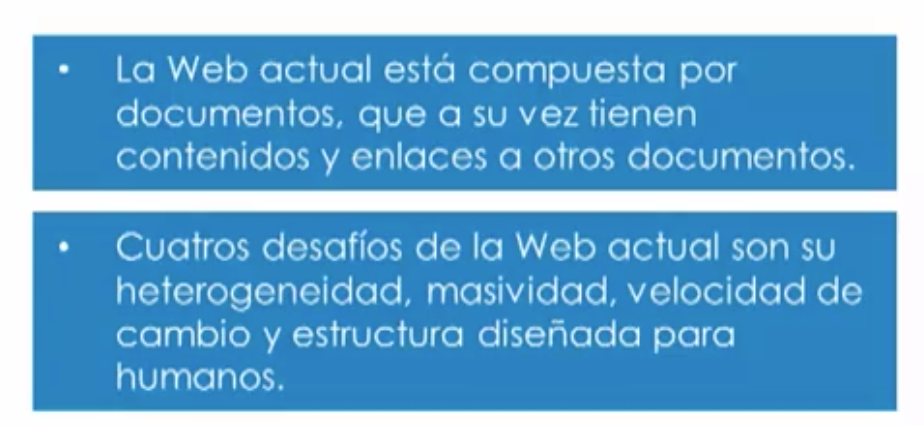
\includegraphics[height=4.5cm]{imagenes/capitulo3/3} % Información sobre la WEB
	\caption{}
\end{figure}

\begin{figure}[H]
	\centering
	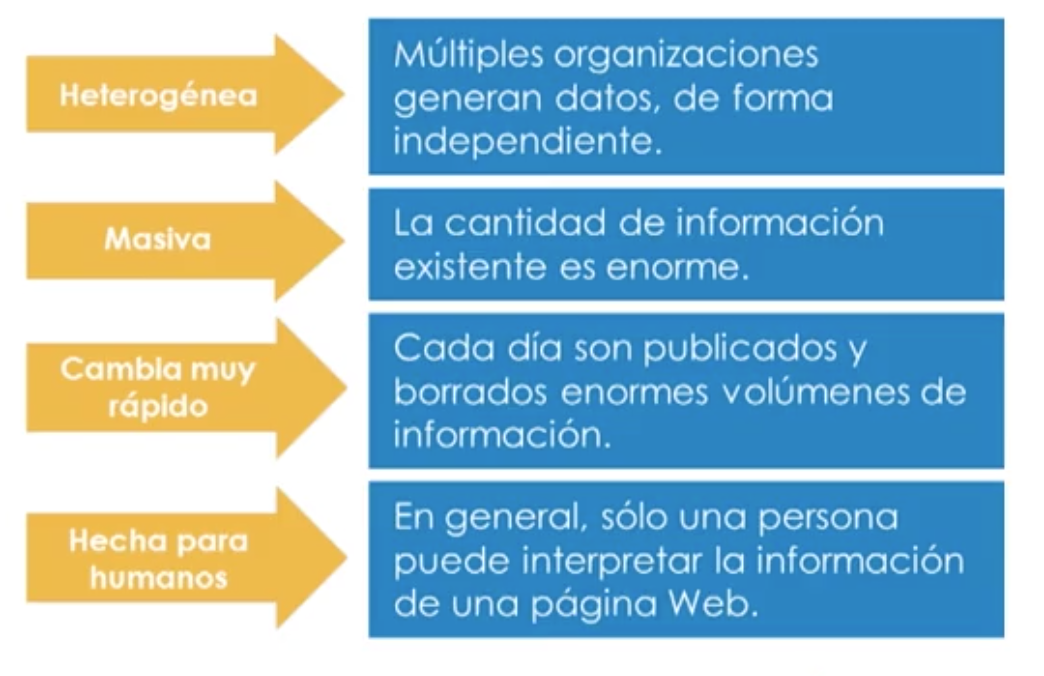
\includegraphics[height=4.5cm]{imagenes/capitulo3/1} % Características de la WEB
	\caption{}
\end{figure}

% DESAFÍOS O CARACTERÍSTICAS DE LA WEB

% COURSERA: La Web Semántica: Herramientas para la publicación y extracción efectiva de información en la Web
\begin{enumerate}
	
	% Heterogenea
	\item Más en detalle la web es heterogénea porque cada aplicación web, cada página web crea los datos y los presenta a los usuarios de una forma totalmente distintas. Es distinto lo que se hace en Facebook, en LinkedIn, en Orkut, en MySpace. Todas esas son redes sociales. Son totalmente distintas y no intercambian datos entre ellas.
	
	% Masiva
	\item Además la web es masiva. Hay muchísimos datos en PubMed, en Wikipedia, en Facebook. Hay una cantidad ingente de datos. Además cambia muy rápido. Por ejemplo, yo podría estar actualizando mi perfil de Facebook cada hora, cada dos horas. Hay gente que lo actualiza cada 15 minutos. Entonces todo esto cambia muy rápido y estoy dando un ejemplo muy chiquito, muy concreto. Además la web es masiva. Por ejemplo, la Wikipedia son casi 6 terabytes de datos. Y ¿qué es un terabyte de datos? En un terabyte de datos caben 678 millones de páginas de texto. 678 millones, eso, suponiendo que el Quijote tiene 1.000 páginas de texto, quiere decir que en un terabyte caben 678 mil Quijotes, Y en una Wikipedia, con 6 terabytes de datos, caben alrededor de 4 millones de Quijotes. Muchísimo.
	
	% Cambia muy rápido
	\item La web actual cambia muy rápido. Actualmente se transfieren en Internet 160 terabytes de datos por segundo. Esos son 27 Wikipedias por segundo. Se transfieren alrededor de Internet 27 Wikipedias cada segundo. Eso es muchísimo.
	
	% Hecha para humanos
	\item Y sobre todo, la web actual está hecha para humanos. Si nos hemos fijado hasta el momento, los ejemplos que he puesto, la Wikipedia, PubMe,d Facebook, todo esto está hecho para que sea consumido por humanos. Las máquinas, el software no tiene tanto acceso a este contenido. Es difícil para un programa interpretar los datos que hay, por ejemplo, en el perfil de Facebook de una persona. o dentro de la Wikipedia. Además la web está hecha para humanos. Como comentaba anteriormente Facebook lo consumen principalmente las personas. La Wikipedia la consumen normalmente las personas. Pero ¿qué pasa si yo quiero enlazar o combinar los datos de la Wikipedia y de Facebook o la Wikipedia y de PubMed? Eso actualmente, con el diseño de la web actual no es posible.
	
	\begin{figure}[H]
		\centering
		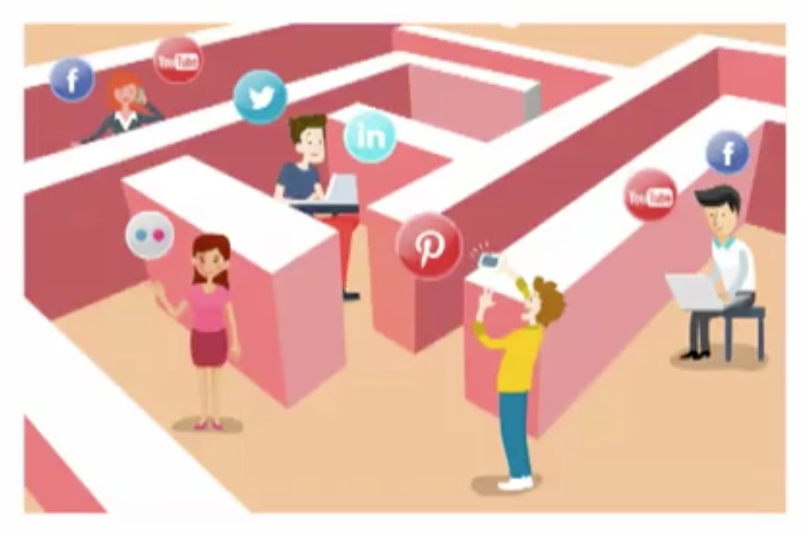
\includegraphics[height=4.5cm]{imagenes/capitulo3/2} % Ejemplo gráfico de humano
		\caption{}
		\label{}
	\end{figure}

\end{enumerate}


% COURSERA: La Web Semántica: Herramientas para la publicación y extracción efectiva de información en la Web
Entonces ¿cómo podría una aplicación consumir datos de dos webs distintas? Leyendo el texto, el contenido. Pero, ¿cómo sabe qué texto leer? ¿Cómo sabe qué contenido leer dentro de una página web? Mirando el código de la html de cada página web. Podría ser pero es muy desordenado. Por dentro el código está muy desordenado siempre. Uno no sabe, una aplicación no sabría exactamente dónde está el nombre de una persona dentro del código html. Normalmente es muy difícil de saber.

% COURSERA: La Web Semántica: Herramientas para la publicación y extracción efectiva de información en la Web
Entonces, para resumir hemos visto que la web es masiva, está compuesta por documentos. Estos documentos tienen contenido y enlaces a otras páginas web. Hay varios desafíos dentro de la web actual que son la heterogeneidad, la velocidad de cambio, la masividad de la web. Y que está hecha para humanos. Un software, una aplicación no sabe identificar o consumir los datos de una página web.

% COURSERA: La Web Semántica: Herramientas para la publicación y extracción efectiva de información en la Web
Entonces, estos son los desafíos que intenta resolver la web semántica. Sobre todo la parte de la heterogeneidad de datos y la parte de que está hecha para los humanos. La web semántica va a tratar de derribar las barreras que existen en la web actual para que los contenidos puedan ser consumidos por máquinas de manera mucho más eficiente.

% ENTENDER LA WEB ACTUAL (RESUMEN DEL PARRAFO)

% COURSERA: La Web Semántica: Herramientas para la publicación y extracción efectiva de información en la Web
En este curso verá en que consisten las tecnologías de la Web Semántica y como se utilizan en la web actual. También tendrá la oportunidad de realizar varios proyectos aplicando todas estas tecnologías para resolver los problemas que Marcelo ha comentado anteriormente. Por ejemplo, ¿le gustaría que Google entendiera cada uno de los componentes de su página web? O si usted tienen una tienda virtual, ¿le gustaría que Google fuera capaz de identificar los distintos productos que forman parte de su tienda virtual y los desplegara al momento de hacer una búsqueda? Esto se consigue usando [DESCONOCIDO] y les mostraremos como se relaciona en este curso con las tecnologías de la Web Semántica.

% COURSERA: La Web Semántica: Herramientas para la publicación y extracción efectiva de información en la Web
Además, ¿le gustaría poder acceder a la Wikipedia como si fuera una tabla Excel? ¿O le gustaría poder conocer como han hecho los gobiernos para hacer públicos sus datos y de esta manera permitir que los ciudadanos puedan acceder a la información de como se gastan sus impuestos, o puedan entender de una manera más sencilla como le afecta una ley? ¿O le gustaría saber como hacen los biólogos para compartir sus datos en la web?


\subsection{Tipos de Web} % Evolución de la Web

% hablar sobre los tipos de web, según veo hay Web 1.0, Web 2.0 y Web 3.0 o Semántica

% https://www.hazhistoria.net/blog/historia-del-www-de-la-web-10-la-web-30

% evolucion de la web: http://profesores.elo.utfsm.cl/~tarredondo/info/networks/Evolucion_Web.pdf

% Web 3.0: integración de la Web Semántica y la Web 2.0:  http://www.albertolsa.com/wp-content/uploads/2009/07/redessociales-web-30-integracion-de-la-web-semantica-y-la-web-20-los-santos-nava-godoy.pdf

\begin{figure}[H]
	\centering
	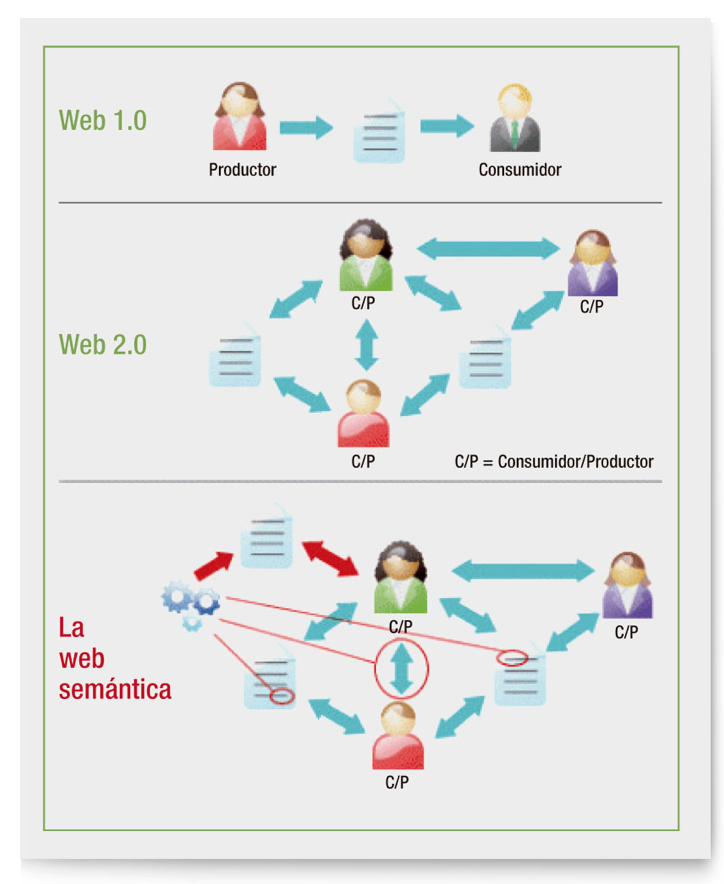
\includegraphics[height=4.5cm]{imagenes/capitulo3/10}
	\caption{}
\end{figure}
% Evolución de una web cuyo contenido es producido por unos y consumidos por otros a una web semántica que mejora la cooperación entre computadoras y humanos.

% http://www.fgcsic.es/lychnos/es_es/articulos/construyendo_una_web_semantica
A partir de ahí podemos ir saltando de una página web a otra a través de hipervínculos –estas palabras, frases, imágenes o iconos que generan la descarga automática de otra página web cuando pinchamos sobre ellos–. Esto es lo que se conoce como la web de primera generación o Web 1.0: personas con conocimiento especializado de diseño y composición de páginas web crean los documentos con su contenido y definen los hipervínculos que los entrelazan; los usuarios no expertos son fundamentalmente consumidores de información. Leen noticias, consultan diccionarios, visualizan imágenes o vídeos o compran productos. 

% http://www.fgcsic.es/lychnos/es_es/articulos/construyendo_una_web_semantica
En la web de segunda generación, la Web 2.0, los usuarios no expertos, además de consumidores, pueden ser también generadores de contenidos y proveedores de servicios. Mediante blogs, por ejemplo, se pueden escribir y compartir reflexiones periódicas, y los lectores pueden añadir comentarios o nuevos enlaces relevantes; con Wikipedia, millones de personas construyen una gran enciclopedia multilingüe que constantemente es actualizada y ampliada por los propios usuarios; a través de redes entre pares, como originalmente Napster, BitTorrent o eMule, se comparten películas y ficheros de música; y últimamente, con la irrupción de las redes sociales —Facebook, Tuenti o Twitter—, la Web se ha convertido en un espacio global de participación e interacción entre usuarios.

% http://www.fgcsic.es/lychnos/es_es/articulos/construyendo_una_web_semantica
La web semántica viene a ser la tercera generación de la Web, la Web 3.0, una extensión de la Web actual en la que los contenidos están organizados de forma que no solo los humanos sino también las computadoras sean capaces de procesar su significado —por eso lo de semántica— posibilitando así una mejor cooperación entre computadoras y humanos. La nomenclatura Web 1.0, 2.0 y 3.0 es seguramente artificiosa, ya que de hecho no se trata de nuevas versiones de la Web, sino de la misma web de siempre pero con niveles añadidos de funcionalidad. 

% https://www.weblaspalmas.es/noticias-tecnologicas/172/La-web-3-0-De-la-web-social-a-la-semantica.html

% Meter algo en el principio de este apartado y luego continuar escribiendo en el apartado de la web semántica
% http://personales.upv.es/ccarrasc/doc/2002-2003/WebSem/WS_2_b.htm#_Toc41588970

% Las web 3.0: de la web social a la semántica: https://www.puromarketing.com/12/15656/social-semantica.html

\section{¿Qué es la Web Semántica?}

% https://wiki.dbpedia.org/

% http://inteligencia-artificial-unsxx.blogspot.com/p/web-semantica-y-web-30.html

La Web Semántica permitirá a las máquinas comprender documentos y datos semánticos, pudiendo asÍ colaborar entre ellas y con las personas.\\

La Web Semántica no es una Web aparte, es una extensión de la Web actual que permite que los datos tengan un significado bien definido, de manera que personas y ordenadores puedan trabajar en cooperación más fácilmente.

% tengo que ver como meter el apartado de 1.4 del Capítulo 1 

\subsection{Introducción}

% COURSERA

% COURSERA: La Web Semántica: Herramientas para la publicación y extracción efectiva de información en la Web
Como habíamos visto en el video anterior, hay datos de todo tipo en la web, tenemos datos genéricos, datos médicos, noticias, datos fundamentales. Y en general, estos datos son de fácil acceso de las personas. En general las páginas web están diseñadas para que sean leídas por personas y formatos adecuados para que las personas puedan acceder a la información. Pero tenemos un problema, la cantidad de datos es tan grande que no la podemos manejar. Solo piensa en los datos que a los cuales usted accede a la web. Por ejemplo tiene el correo electrónico, puede crear una página en Facebook, puede tener información en Instagram, puede acceder a información en Wikipedia y en información general, puede acceder a información geográfica, etcétera, etcétera. ¿Sí? Veamos algunos ejemplos de estos datos en la web. 

\begin{figure}[H]
	\centering
	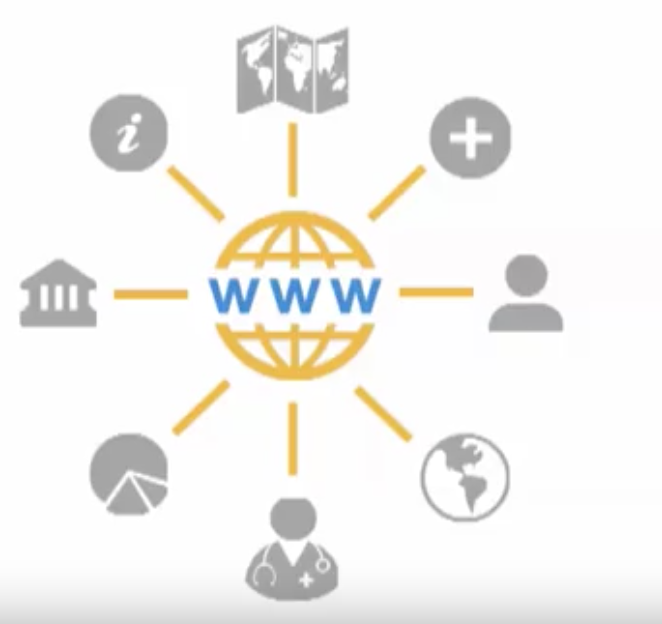
\includegraphics[height=4.5cm]{imagenes/capitulo3/4}
	\caption{}
\end{figure}

\begin{figure}[H]
	\centering
	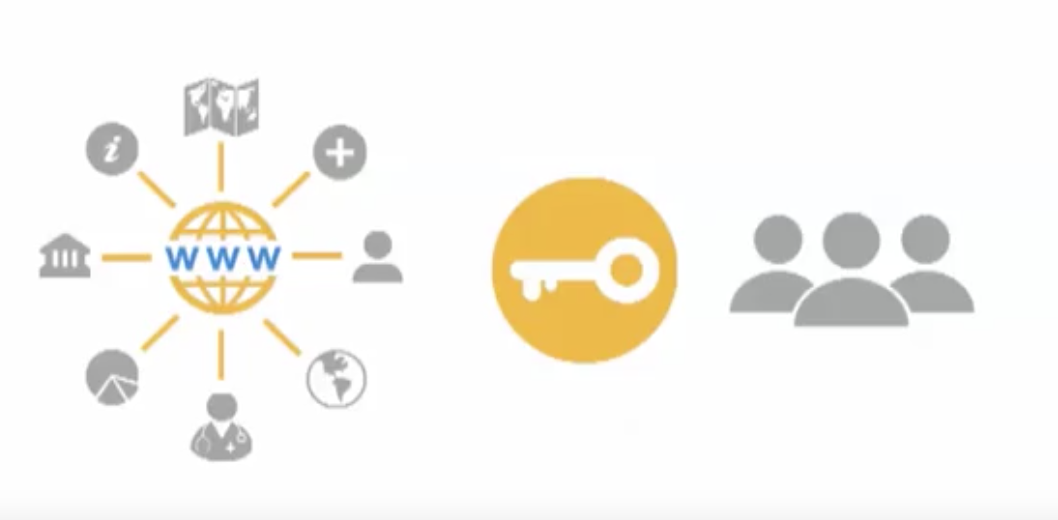
\includegraphics[height=4.5cm]{imagenes/capitulo3/5}
	\caption{}
\end{figure}

\begin{figure}[H]
	\centering
	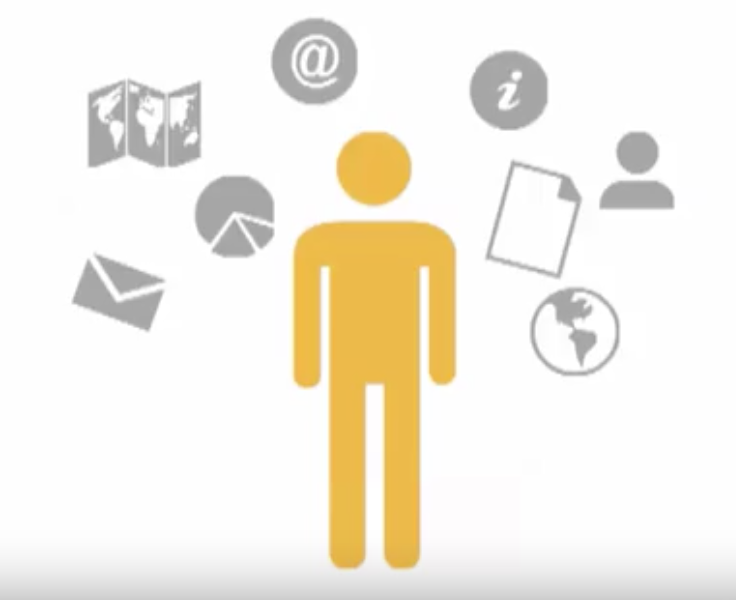
\includegraphics[height=4.5cm]{imagenes/capitulo3/6}
	\caption{}
\end{figure}

% COURSERA: La Web Semántica: Herramientas para la publicación y extracción efectiva de información en la Web
En primer lugar tenemos datos genéricos como el ejemplo en Wikipedia. En Wikipedia podemos encontrar información sobre todo tipo de elementos, por ejemplo información geográfica, información sobre historia de los países, información sobre, información científica, etcétera, etcétera. Si bien en algún lugar también tenemos datos médicos, por ejemplo tenemos la biblioteca nacional de medicina de Estados Unidos, donde acá uno puede encontrar información sobre enfermedades, sobre tratamientos, sobre síntomas, etcétera. También tenemos noticias y en esto probablemente usted todos los días lee algún diario que está publicado en la web, por ejemplo The New York Times. También tenemos datos gubernamentales, los distintos gobiernos han decidido tener leyes de transparencia que han obligado a las distintas agencias de estos gobiernos a publicar datos en la web. Por ejemplo, en esta transparencia podemos ver el London Data store, donde la ciudad de Londres guarda información gubernamental, por ejemplo información sobre transporte, sobre salud pública, etcétera.

% COURSERA: La Web Semántica: Herramientas para la publicación y extracción efectiva de información en la Web
Entonces, ¿cómo podemos aprovechar estos datos? Algo que es importante tener en cuenta en este momento, es que los computadores tienen la capacidad para poder analizar estos datos, tenemos suficientes computadores, tenemos suficientes procesadores como para organizar esta información. Pero, ¿cuál es el problema que tenemos actualmente? Es que los capaces, los computadores no son capaces de interpretar la información que está en estas páginas web, o sea, las páginas están pensadas para ser leídas por personas no por computadores. Entonces, ¿qué es lo que necesitamos hacer? Hay que permitir que las aplicaciones computacionales entiendan los datos. Y aquí la pregunta fundamental es, ¿cómo podemos hacer esto?

% COURSERA: La Web Semántica: Herramientas para la publicación y extracción efectiva de información en la Web
Entonces, ¿cuáles son los requisitos para una web de datos efectiva por una web donde los computadores y las personas puedan acceder y entender la información? En primer lugar, es necesario tener un lenguaje que nos permita especificar los recursos que tenemos en la web y cuáles son las relaciones que existen entre ellos. ¿Sí? Con recurso me refiero a los distintos componentes de la web, esto puede ser una página web, un diario, una persona que tiene una página web, etcétera. Y queremos también especificar cuáles son las relaciones que existen entre ellos. Por ejemplo, esta noticia fue publicada en este diario, esta página de aquí, esta página por ejemplo tiene información sobre problemas de salud en este determinado país, etcétera, etcétera. Ahora un requisito fundamental para diseñar este lenguaje que nos permita especificar recursos, sus relaciones es que el debe ser procesable por un computador. Un computador, una aplicación computacional debe entender este lenguaje. En segundo lugar, necesitamos poder consultar estos datos mediante aplicaciones computacionales y con esto nos referimos a poder especificar lo que estamos buscando y que de manera automática se extraiga esta información. Aquí nuevamente tenemos dos requisitos fundamentales, debemos tener un lenguaje para describir consultas que sea procesable por un computador de nuevo vamos a describir una consulta en un cierto lenguaje y lo que esperamos que el computador entienda o la aplicación computacional entienda esta consulta y debemos ser capaz de sacar conclusiones a partir de los datos de manera automáticos. Debemos ser capaces de extraer de manera automática la respuesta a la consulta o la respuesta a las consultas que estamos realizando.

\begin{figure}[H]
	\centering
	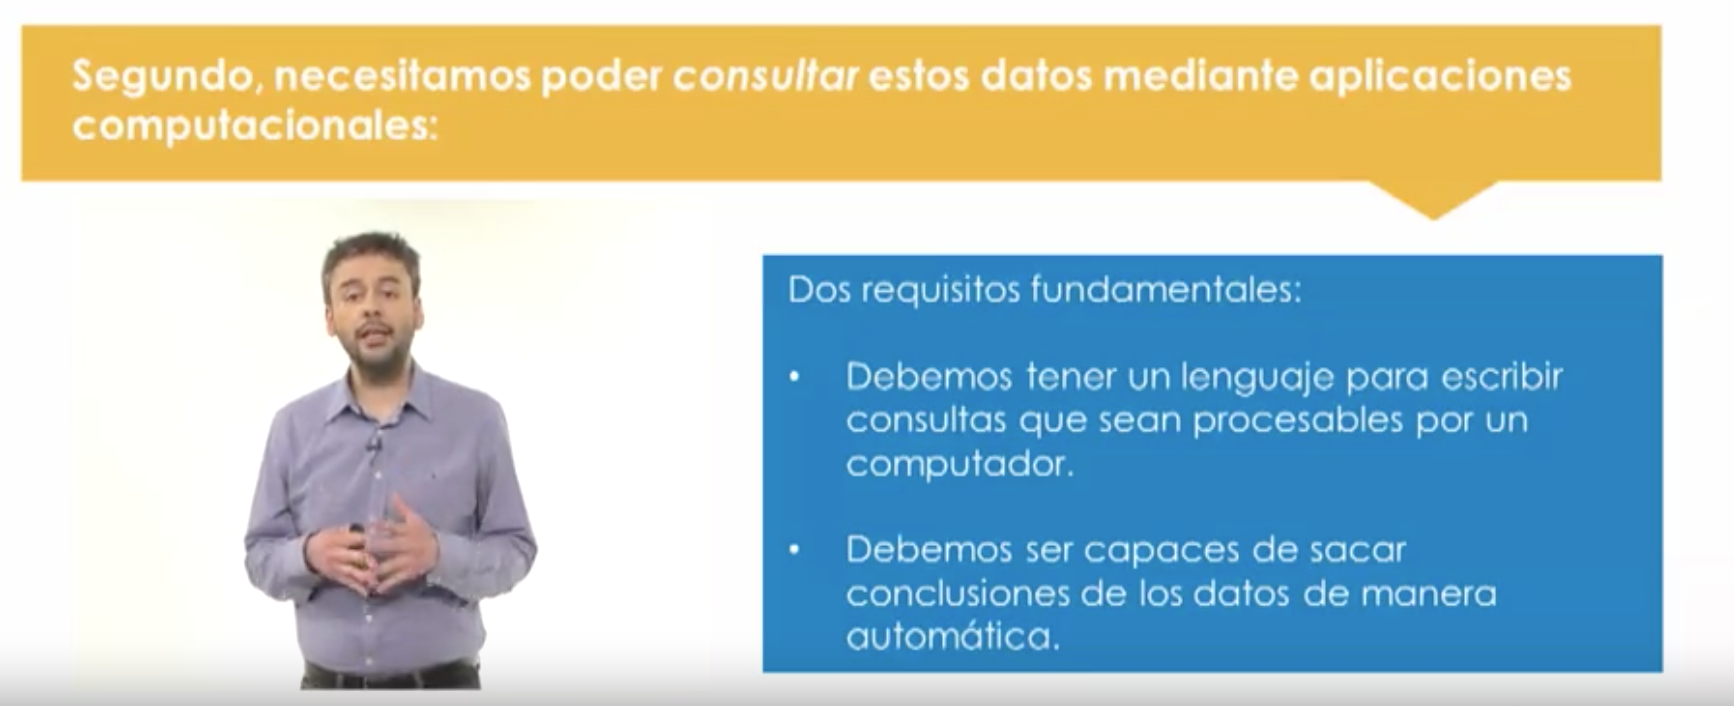
\includegraphics[height=4.5cm]{imagenes/capitulo3/7}
	\caption{}
\end{figure}


En mayo de 2001 la revista Scientific American publicaba un artículo en el que se proponía una nueva forma de organizar el contenido en la Red que desencadenaría una avalancha de posibilidades y, en consecuencia, revolucionaría Internet. El primer autor del artículo era Tim Berners-Lee, el físico del CERN que en 1980 desarrolló un sistema de vinculación y transferencia de documentos en red que acabó convirtiéndose en la World Wide Web que todos conocemos hoy. A la nueva forma de organización de la Web que los autores de dicho artículo pregonaban la llamaron web semántica. % http://www.fgcsic.es/lychnos/es_es/articulos/construyendo_una_web_semantica

% COURSERA: La Web Semántica: Herramientas para la publicación y extracción efectiva de información en la Web
En este punto es donde aparece la web semántica en este curso, en palabras de Tim Berners-Lee la web semántica es una extensión de la web actual en la cual se da un significado bien definido a la información, permitiendo mejorar la colaboración entre personas y computadores en la web. ¿En qué se traduce esto en la práctica? Bueno, la web semántica en la práctica lo que vemos hoy en día es un conjunto de recomendaciones desarrolladas por el World Wide Web Consortium, cuyo objetivo es que los computadores sean capaces de entender los datos en la web. Aquí tenemos que detenernos en dos conceptos importantes. En primer lugar, ¿qué es una recomendación? En este nivel, una recomendación es una descripción formal de una tecnología que debería ser utilizada por todos. ¿Sí? Es decir, un lenguaje común para todos. Lo que queremos hacer en este punto es desarrollar un lenguaje que por ejemplo nos permita especificar los recursos de la web que tenga una descripción formal, para que así pueda ser entendida por un computador y que sea un lenguaje común para todos. También es importante mencionar acá que el World Wide Web Consortium es el organismo regulador de la web, es el organismo que dicta los distintos estándares para la web.

\begin{figure}[H]
	\centering
	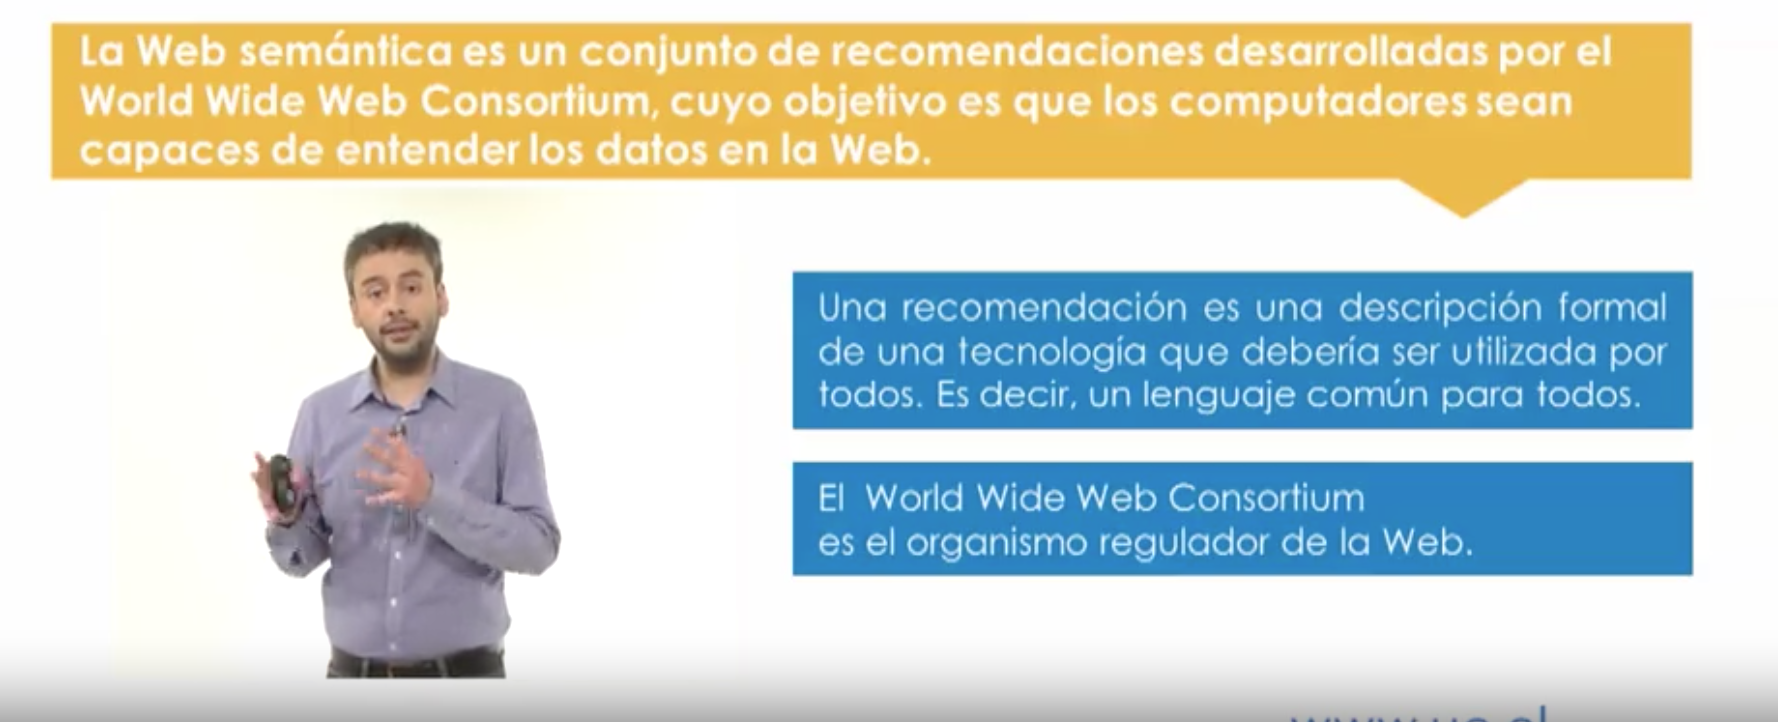
\includegraphics[height=4.5cm]{imagenes/capitulo3/8}
	\caption{}
\end{figure}

Han pasado más de diez años y es bien seguro que la Web ha revolucionado muchos aspectos de nuestras vidas cotidianas, pero la revolución que se preveía en el artículo del Scientific American todavía no se ha producido, por lo menos no en su totalidad. Sin embargo, la visión de una web semántica que describieron Berners-Lee y sus colaboradores desencadenó toda un línea de proyectos de investigación, y, precisamente, en octubre pasado se celebró en Bonn, Alemania, la 10ª edición del Congreso Internacional sobre la Web Semántica. Pero, ¿qué significa que la Web sea semántica? Y ¿en qué medida la semántica en la Web ya ha revolucionado o acabará por revolucionar Internet? % http://www.fgcsic.es/lychnos/es_es/articulos/construyendo_una_web_semantica

Ahora, ¿cuáles son esos estándares para la web? En la figura usted puede observar la pirámide de estándares que se está desarrollando para llevar a cabo esta web semántica. Y en esta pirámide en la parte inferior vemos los componentes más básicos, en la parte superior donde vemos el trust o el nivel de confianza ve uno en los niveles superiores. En este curso nos vamos a centrar en cuatro de estos componentes de esta pirámide que están marcados con colores. En primer lugar vamos a ver RDF, que es el lenguaje básico para especificar recursos de la web y sus relaciones, RDFS que nos permite decir un poco más vamos a hablar de este vocabulario, SPARQL que es este lenguaje de consulta que nos permite extraer información desde la web y finalmente OWL o este lenguaje que nos permite identificar ontologías.


El potencial de la web de datos, al igual que pasó con la web de documentos, reside en la participación a gran escala de numerosas personas y organizaciones en la publicación sistemática de datos en la Web, siguiendo las buenas prácticas de Linked Data. Es esta participación masiva, con un esfuerzo relativamente bajo, la que está detrás del éxito de la Web actual. La publicación de datos es solo una parte de lo que constituye la web de datos. La otra parte la forman las aplicaciones informáticas que nos proveen de los servicios para acceder, consultar, buscar y combinar los datos. Al igual que la web de documentos no nos sería de gran utilidad sin navegadores, buscadores o servicios de interacción social, las funcionalidades de la web de datos nos las dan las aplicaciones determinadas sobre los datos enlazados que utilizan leguajes específicos de consulta en repositorios RDF, tales como SPARQL, que se inspira en el leguaje SQL (Structured Query Language) de consulta de bases de datos tradicionales, pero ahora especialmente diseñado para ser ejecutado sobre la tecnología web. % http://www.fgcsic.es/lychnos/es_es/articulos/construyendo_una_web_semantica

\begin{figure}[H]
	\centering
	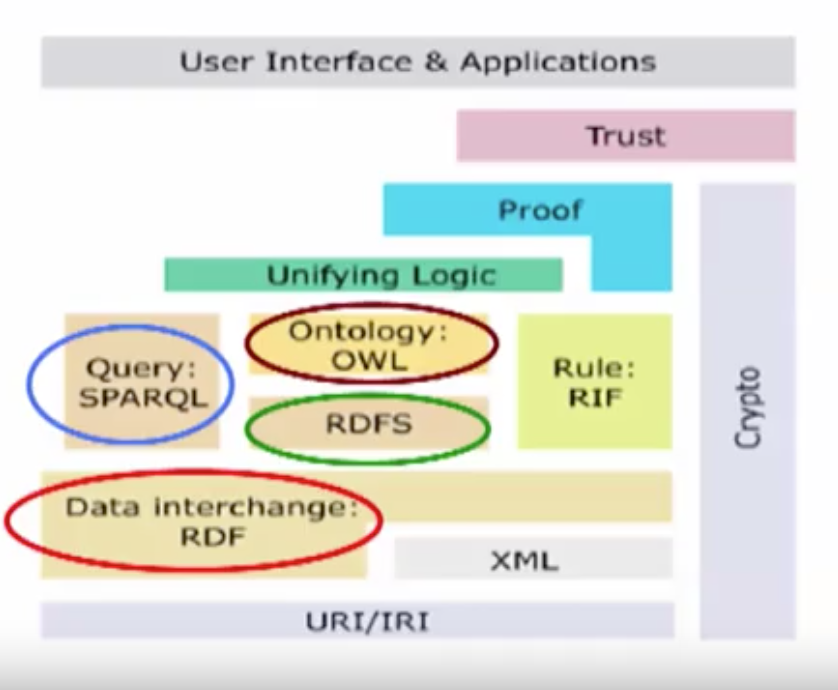
\includegraphics[height=4.5cm]{imagenes/capitulo3/9}
	\caption{}
\end{figure}

En resumen, ¿qué hemos visto hoy? Hemos visto que hay datos de todo tipo en la web, que son fácil acceso para las personas. Hemos visto que la cantidad de datos es tan grande que las personas no lo pueden manejar en su totalidad, son demasiados para que una persona simplemente pueda procesarlos por sí sola. También hemos visto que es difícil para un computador acceder a estos datos ya que no sabe como interpretarlos. La web de hoy en día está diseñada para ser leídas por personas, las páginas web están diseñadas para ser leídas por personas. ¿Sí? Y no está diseñada para que un computador las pueda leer de manera automática. Y finalmente la web semántica, que es el tema de este curso hemos visto que es un conjunto de recomendaciones para facilitar el acceso de los computadores a los datos. En particular, lo que queremos en este punto es tener el lenguaje que nos permita especificar los recursos que tenemos en la web, especificar las relaciones que tenemos entre ellos y también definir lenguajes que nos permitan extraer de manera automática de esta web.

% https://www.researchgate.net/publication/216537707_La_Web_semantica_y_las_tecnologias_del_lenguaje_humano
La implantación de la web semántica frente a la actual web supone un cambio de paradigma, ya que tiene que pasarse de una web basada y creada en lenguaje natural a una web estructurada y organizada, donde los contenidos etiquetados semánticamente serán el elemento principal. Este cambio supondrá una nueva filosofía y forma de trabajar, ya que el desarrollo y creación de contenidos para esta web requerirá una gran cantidad de esfuerzos. Es en este punto donde pueden intervenir las tecnologías del lenguaje humano para facilitar mecanismos y herramientas que ayuden a la implantación y expansión de este nuevo paradigma.

% DECIR EN CIERTA MEDIDA QUE VAMOS A VER DE LA WEB SEMÁNTICA

% https://disenowebakus.net/semantica-web.php
Para conocer que es la Web semántica, es necesario establecer los principios básicos, tanto conceptuales como tecnológicos sobre los que se asienta. Además de saber con precisión a qué nos referimos cuando utilizamos la expresión "Web semántica", también resulta esencial conocer su arquitectura a través de un modelo que muestre tanto sus elementos, como la dinámica en torno a la cual se articulan los diferentes desarrollos tecnológicos que nos han llevado desde la Web original hasta la Web semántica.

% COURSERA: La Web Semántica: Herramientas para la publicación y extracción efectiva de información en la Web
Entonces, ¿cómo podemos aprovechar estos datos? Algo que es importante tener en cuenta en este momento, es que los computadores tienen la capacidad para poder analizar estos datos, tenemos suficientes computadores, tenemos suficientes procesadores como para organizar esta información. Pero, ¿cuál es el problema que tenemos actualmente? Es que los capaces, los computadores no son capaces de interpretar la información que está en estas páginas web, o sea, las páginas están pensadas para ser leídas por personas no por computadores. Entonces, ¿qué es lo que necesitamos hacer? Hay que permitir que las aplicaciones computacionales entiendan los datos. Y aquí la pregunta fundamental es, ¿cómo podemos hacer esto?

% COURSERA: La Web Semántica: Herramientas para la publicación y extracción efectiva de información en la Web
Entonces, ¿cuáles son los requisitos para una web de datos efectiva por una web donde los computadores y las personas puedan acceder y entender la información? En primer lugar, es necesario tener un lenguaje que nos permita especificar los recursos que tenemos en la web y cuáles son las relaciones que existen entre ellos. ¿Sí? Con recurso me refiero a los distintos componentes de la web, esto puede ser una página web, un diario, una persona que tiene una página web, etcétera. Y queremos también especificar cuáles son las relaciones que existen entre ellos. Por ejemplo, esta noticia fue publicada en este diario, esta página de aquí, esta página por ejemplo tiene información sobre problemas de salud en este determinado país, etcétera, etcétera. Ahora un requisito fundamental para diseñar este lenguaje que nos permita especificar recursos, sus relaciones es que el debe ser procesable por un computador. Un computador, una aplicación computacional debe entender este lenguaje. En segundo lugar, necesitamos poder consultar estos datos mediante aplicaciones computacionales y con esto nos referimos a poder especificar lo que estamos buscando y que de manera automática se extraiga esta información. Aquí nuevamente tenemos dos requisitos fundamentales, debemos tener un lenguaje para describir consultas que sea procesable por un computador de nuevo vamos a describir una consulta en un cierto lenguaje y lo que esperamos que el computador entienda o la aplicación computacional entienda esta consulta y debemos ser capaz de sacar conclusiones a partir de los datos de manera automáticos. Debemos ser capaces de extraer de manera automática la respuesta a la consulta o la respuesta a las consultas que estamos realizando.

% https://www.researchgate.net/publication/216537707_La_Web_semantica_y_las_tecnologias_del_lenguaje_humano
La semántica es considerada uno de los elementos clave de esta nueva fase de la web, ya que es donde reside gran parte de su potencial, pues a partir de la manipulación de elementos dotados de valor semántico pueden ofrecerse nuevos servicios que aún no existen en la actual web. De esta manera, las tecnologías semánticas, estrechamente relacionadas con las tecnologías del lenguaje humano, se han convertido en uno de los pilares de este nuevo paradigma, ya que pueden ayudar a su desarrollo e implantación.

% https://www.researchgate.net/publication/216537707_La_Web_semantica_y_las_tecnologias_del_lenguaje_humano
Las tecnologías del lenguaje humano tratan de buscar mecanismos computacionales que permitan reconocer, comprender y generar lenguaje natural, para ello realizan un tratamiento automático de éste. Por tanto, intentan trasladar e integrar el conocimiento que las personas tenemos de la lengua en los agentes para que puedan emular las acciones que podemos realizar de forma innata. Para lograr este objetivo incorporan modelos teóricos, métodos y técnicas de diferentes disciplinas: lingüística, filosofía, psicología e ingeniería, ya que todas ellas están implicadas o pueden resultar útiles para tratar los diferentes procesos que envuelven el lenguaje natural. Cada una de ellas estudia la lengua desde puntos de vista y objetivos distintos, lo cual ha conllevado también el uso de terminología diferente para hacer referencia a la misma idea. La lingüística utiliza el término ‘lingüística computacional’, la ingeniería informática usa la expresión ‘ingeniería del lenguaje natural’. Sin embargo, el concepto más utilizado tradicionalmente por la comunidad científica es ‘procesamiento del lenguaje natural’, aunque actualmente está muy extendida la expresión ‘tecnologías del lenguaje humano’, especialmente en el marco de la Unión Europea. En este capítulo utilizaremos este último término al resultar más cercano y divulgativo para los profanos en esta disciplina.

% https://www.researchgate.net/publication/216537707_La_Web_semantica_y_las_tecnologias_del_lenguaje_humano
Los contenidos de la actual web deben ser interpretados por las personas, ya que el uso del lenguaje natural como medio de expresión en muchos casos requiere deducir conocimiento implícito de los textos para poder ser comprendidos correctamente. Por ejemplo, para solucionar los problemas de ambigüedad propios del lenguaje natural es necesario contar con información que en algunos casos no está explícita en los textos pero que las personas somos capaces de extraer a partir del contexto.

% https://www.researchgate.net/publication/216537707_La_Web_semantica_y_las_tecnologias_del_lenguaje_humano
El gran reto de la web semántica reside en conseguir que los contenidos estén dotados explícitamente de semántica para que a partir aquí los agentes sean capaces de deducir e inferir conocimiento. Como ya se ha comentado, actualmente todavía estamos en una fase muy embrionaria de la idea y los más pesimistas dudan que se llegue a buen puerto, pues la inteligencia artificial lleva décadas persiguiendo este objetivo sin gran éxito. Pero durante los últimos años, las tecnologías del lenguaje humano han madurado bastante y han logrado aplicaciones robustas y escalables que pueden ocupar un papel destacado en el desarrollo de la web semántica.

\subsection{Definición}

% https://www.ceupe.com/blog/que-es-la-la-web-semantica.html
% https://disenowebakus.net/semantica-web.php

% Por web semántica se entiende una forma de organizar el contenido en la Web que mejore la cooperación entre computadoras y humanos. Esto pasa por avanzar de una web de documentos a una web de datos enlazados en la que se puedan ofrecer novedosos servicios que hagan uso del potencial de combinar e interrelacionar datos de diversa índole y procedencia.

% Interesante como viene aquí la arquitectura: http://www.mclibre.org/consultar/xml/lecciones/web-semantica.html

% LA PRIMERA DEFINICIÓN SENCILLA SERÍA DEFINIR QUE ES LA WEB Y LUEGO QUE ES LA SEMÁNTICA

% EMPEZAMOS A DEFINIR - PRIMERA DEFINICIÓN LA OFICIAL (VER OTRAS DE LA LITERATURA)

% COURSERA: La Web Semántica: Herramientas para la publicación y extracción efectiva de información en la Web
En este punto es donde aparece la web semántica en este curso, en palabras de Tim Berners-Lee la web semántica es una extensión de la web actual en la cual se da un significado bien definido a la información, permitiendo mejorar la colaboración entre personas y computadores en la web. ¿En qué se traduce esto en la práctica? Bueno, la web semántica en la práctica lo que vemos hoy en día es un conjunto de recomendaciones desarrolladas por el World Wide Web Consortium, cuyo objetivo es que los computadores sean capaces de entender los datos en la web. Aquí tenemos que detenernos en dos conceptos importantes. En primer lugar, ¿qué es una recomendación? En este nivel, una recomendación es una descripción formal de una tecnología que debería ser utilizada por todos. ¿Sí? Es decir, un lenguaje común para todos. Lo que queremos hacer en este punto es desarrollar un lenguaje que por ejemplo nos permita especificar los recursos de la web que tenga una descripción formal, para que así pueda ser entendida por un computador y que sea un lenguaje común para todos. También es importante mencionar acá que el World Wide Web Consortium es el organismo regulador de la web, es el organismo que dicta los distintos estándares para la web.

% DESMENUZANDO LA DEFINICIÓN OFICIAL

% https://disenowebakus.net/semantica-web.php
Podemos identificar varios aspectos clave en esta definición:
\begin{enumerate}
	\item En primer lugar, se refiere a la Web semántica como una extensión de la Web actual. Es decir tanto las nuevas ideas, conceptos y usos de la Web, como las herramientas informáticas utilizadas para el desarrollo de los planteamientos de la Web semántica deben coexistir con el resto de aplicaciones de la Web actual.
	
	\item Otro punto relevante de la definición indica la necesidad de anotar o marcar esta información con datos que proporcionen un significado bien definido (semántica) y compartido para que puedan ser enlazados.
	
	\item La vinculación de datos, representados mediante estándares de la Web semántica permite la reutilización del trabajo realizado por diferentes entidades.
	
	\item De este modo, un tesauro elaborado y publicado en la Web por una institución en un formato apto para la Web semántica, podría ser utilizado por un repositorio digital de otro organismo para signar descriptores de sus registros.
	
	\item En el fondo nos encontramos que en realidad, la Web semántica persigue el desarrollo de mecanismos para que el intercambio de datos entre sistemas y, en última instancia, la comunicación entre hombre máquina, sea eficaz y eficiente.
	
	\item Por último, la misma definición nos adelanta la posibilidad de que los sistemas informáticos podrían ser capaces de manipular e incluso reelaborar información con objetivo concretos a los problemas que se les planteen.
\end{enumerate}

% https://disenowebakus.net/semantica-web.php
La Web semántica no es una Web distinta de la que originalmente fue desarrollada por Tim Berners-Lee. Al igual que la Web 2.0 se trata de un uso concreto de conjuntos de herramientas y tecnologías. Los desarrollos de la Web semántica están basados en una serie de planteamientos e ideas bastante claras. En este sentido, Hendler, Berners-Lee y Miller (2002) ofrecen la siguiente definición de Web semántica: "La web semántica es una extensión de la actual Web en la que a la información disponible se le otorga un significado bien definido que permita a los ordenadores y a las personas trabajar en cooperación. Está basada en la idea de proporcionar en la Web datos definidos y enlazados, permitiendo que aplicaciones heterogéneas localicen, integren, razonen y reutilicen la información presente en la Web."

% https://www.researchgate.net/publication/216537707_La_Web_semantica_y_las_tecnologias_del_lenguaje_humano
El creador del concepto, Tim Berners-Lee, define la web semántica de la siguiente forma: «no es una web separada sino una extensión de la actual, donde la información está dotada de un significado bien definido, los ordenadores están mejor capacitados y las personas trabajan en colaboración» (Berners-Lee, 01). En estas líneas se reúnen los fundamentos de la web semántica: es una evolución de la actual web donde los ordenadores serán capaces de interpretar los documentos ya que estarán dotados de contenido semántico y el trabajo colaborativo será una realidad.

% OTRA DEFINICIÓN

% https://disenowebakus.net/semantica-web.php
Similar definición es la que ofrece Berners-Lee junto con Miller (2002), en la que también exponen el modo en el que el W3C coordina la consecución de estos objetivos: "La Web semántica es una extensión de la actual Web en la que la información disponible se le otorga un significado bien definido que permita a los ordenadores y a las personas trabajar en cooperación. La W3C Semantic Web Activity, en colaboración con un gran número de investigadores y socios industriales, se encarga de la definición de estándares y tecnologías que permitan a los datos de la Web ser definidos y enlazados de forma que puedan ser usados para una localización más eficaz, automatización, integración y reutilización entre aplicaciones."

% OTRA DEFINICIÓN - W3C

% https://disenowebakus.net/semantica-web.php
Desde un enfoque más concreto y retomando la última parte de la definición anterior, podemos encontrar en la página Web oficial que el W3C mantiene sobre la Web semántica el siguiente contenido que puede servir a modo de definición: "La Web semántica es la representación de datos en la Web. Es un esfuerzo colaborativo liderado por W3C con la participación de un gran número de investigadores y socios industriales. Se basa en el uso de RDF, que integra una gran variedad de aplicaciones mediante el uso de XML, para la sintaxis y el uso de URLs para su identificación." 

% DESMENUZANDO LA DEFINICIÓN W3C

% https://disenowebakus.net/semantica-web.php
\begin{enumerate}
	\item Teniendo en cuenta los trabajos de coordinación del W3C es normal que en la definición anterior se incluyan dos tecnologías fundamentales asociadas al desarrollo de la Web semántica: la especificación RDF y el lenguaje XML RDF (Resource Description Framework) es un modelo de datos desarrollado por el W3C que ofrece una especificación para la descripción de metadatos en la Web.
	
	\item Organiza la información en forma de tripletas sujeto-predicado-objeto y permite su expresión sintáctica (serialización) mediante XML.
	
	\item Además también utiliza la expresión URI (Uniform Resource Identifier) para identificar de forma universal y expansible un espacio de nombres de recursos de información.
	
	\item De esta definición también se desprende la existencia de una amplia colaboración, tanto a nivel científico como de diseñadores y fabricante de software, para la adopción y uso de especificaciones comunes referentes a la Web semántica.
\end{enumerate}

% ARQUITECTURA 
% https://www.researchgate.net/publication/216537707_La_Web_semantica_y_las_tecnologias_del_lenguaje_humano
La figura 1 muestra la arquitectura de la web semántica tal como la ha definido Berners- Lee. Se trata de una estructura de capas, donde cada nivel resulta un requisito previo para el siguiente.

\begin{figure}[H]
	\centering
	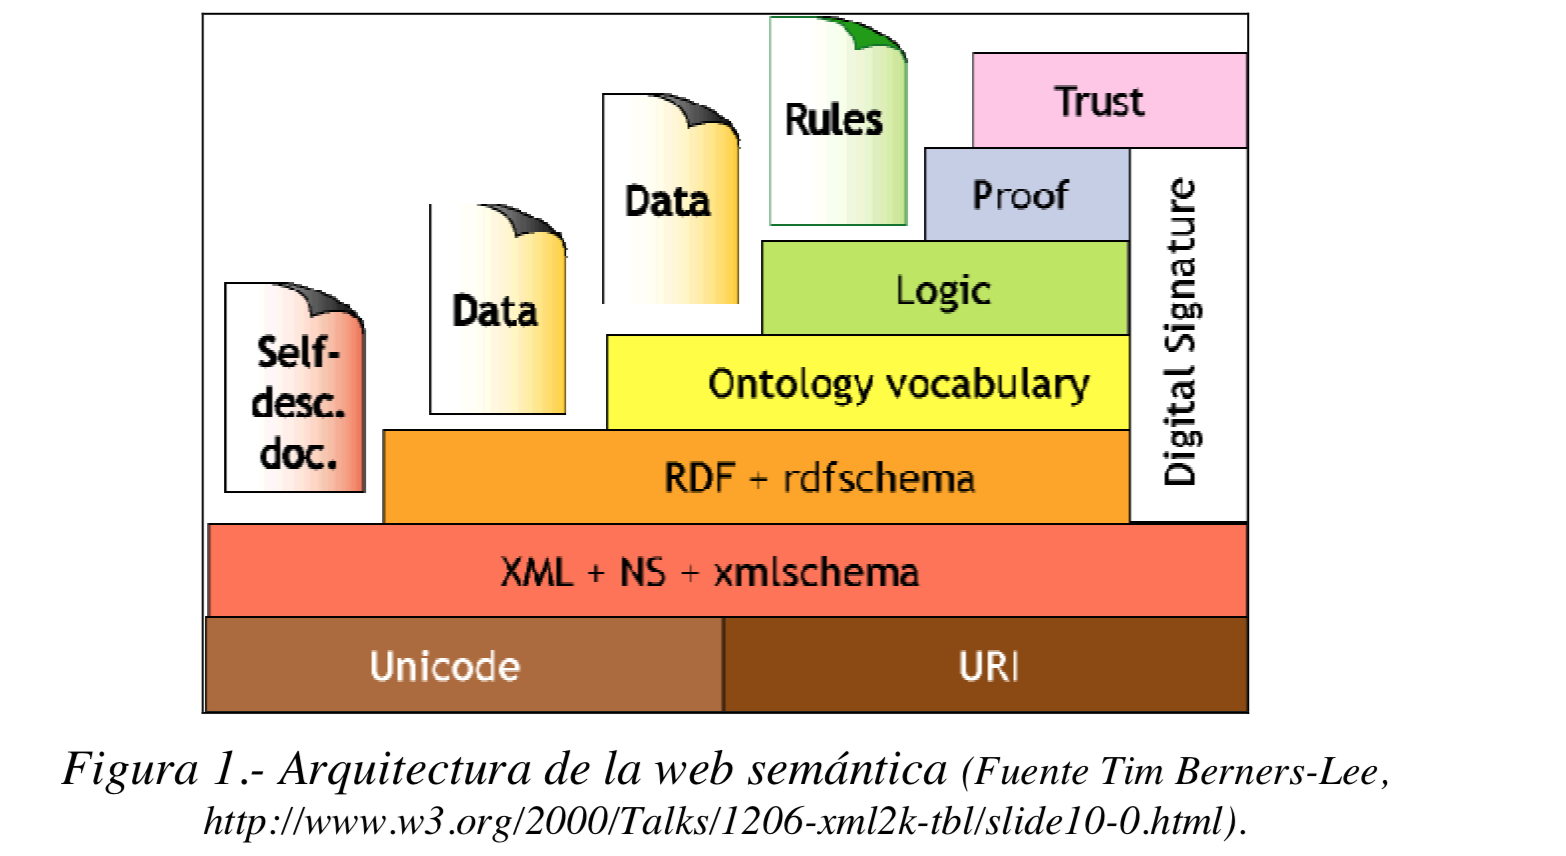
\includegraphics[height=4.5cm]{imagenes/capitulo3/24} % Esquema de los estándares de la Web Semántica
	\caption{}
	\label{}
\end{figure}

% https://www.researchgate.net/publication/216537707_La_Web_semantica_y_las_tecnologias_del_lenguaje_humano
Los dos niveles iniciales hacen referencia a la base y los estándares en los que se sustenta su desarrollo: Unicode, URI, XML y RDF. Éstos permiten convertir la web en una infraestructura global donde será posible compartir y reutilizar datos y documentos entre diferentes tipos de usuarios.

% https://www.researchgate.net/publication/216537707_La_Web_semantica_y_las_tecnologias_del_lenguaje_humano
La siguiente capa, referida a las ontologías, es en donde reside el contenido semántico del sistema. La cuarta capa tiene que permitir, a partir de la estructura semántica generada con las ontologías y los metadatos, realizar inferencias lógicas. Estas dos etapas son las que presentan más incógnitas actualmente y las que pueden actuar como freno para la implantación de la web semántica ya que comportan una infraestructura que actualmente no es posible realizar a gran escala. Es aquí donde las tecnologías del lenguaje humano pueden intervenir ayudando a la creación y mantenimiento de las ontologías y también vinculando éstas con los documentos, pero se trata de un camino aún en fase experimental.


% 6.3.3 La asignación de metadatos

%\section{Tecnologías de la Web Semántica}

%\subsection{Metadatos explícitos}

%Representación más fácilmente procesable por máquinas.

%Metadata: data about data

%Los metadatos representan parte del significado de los datos

%La Web Semántica no se basa en la manipulación de texto, sino en metadatos procesables por las máquinas.

% XML
% RDF

% Ejemplo

% % https://www.researchgate.net/publication/216537707_La_Web_semantica_y_las_tecnologias_del_lenguaje_humano
Uno de los elementos fundamentales de la web semántica son los metadatos; es decir, información/datos que describen los contenidos de los documentos a los que están asociados representando de forma explícita el significado de éstos. El modelo de representación de los metadatos en la web semántica es RDF (Resource Description Framework). Se basa en describir los recursos como expresiones con la forma sujeto- predicado-objeto. El sujeto es el recurso, es decir, aquello que se está describiendo. El predicado es la propiedad o relación que se desea presentar del recurso. Por último, el objeto es el valor de la propiedad o el otro recurso con el que se establece una relación. Esta estructura presenta limitaciones, por eso se combina con RDF Schema y OWL que permite representar relaciones semánticas más complejas que las descritas. La siguiente figura muestra un ejemplo de metadatos en RDF y OWL.

\begin{figure}[H]
	\centering
	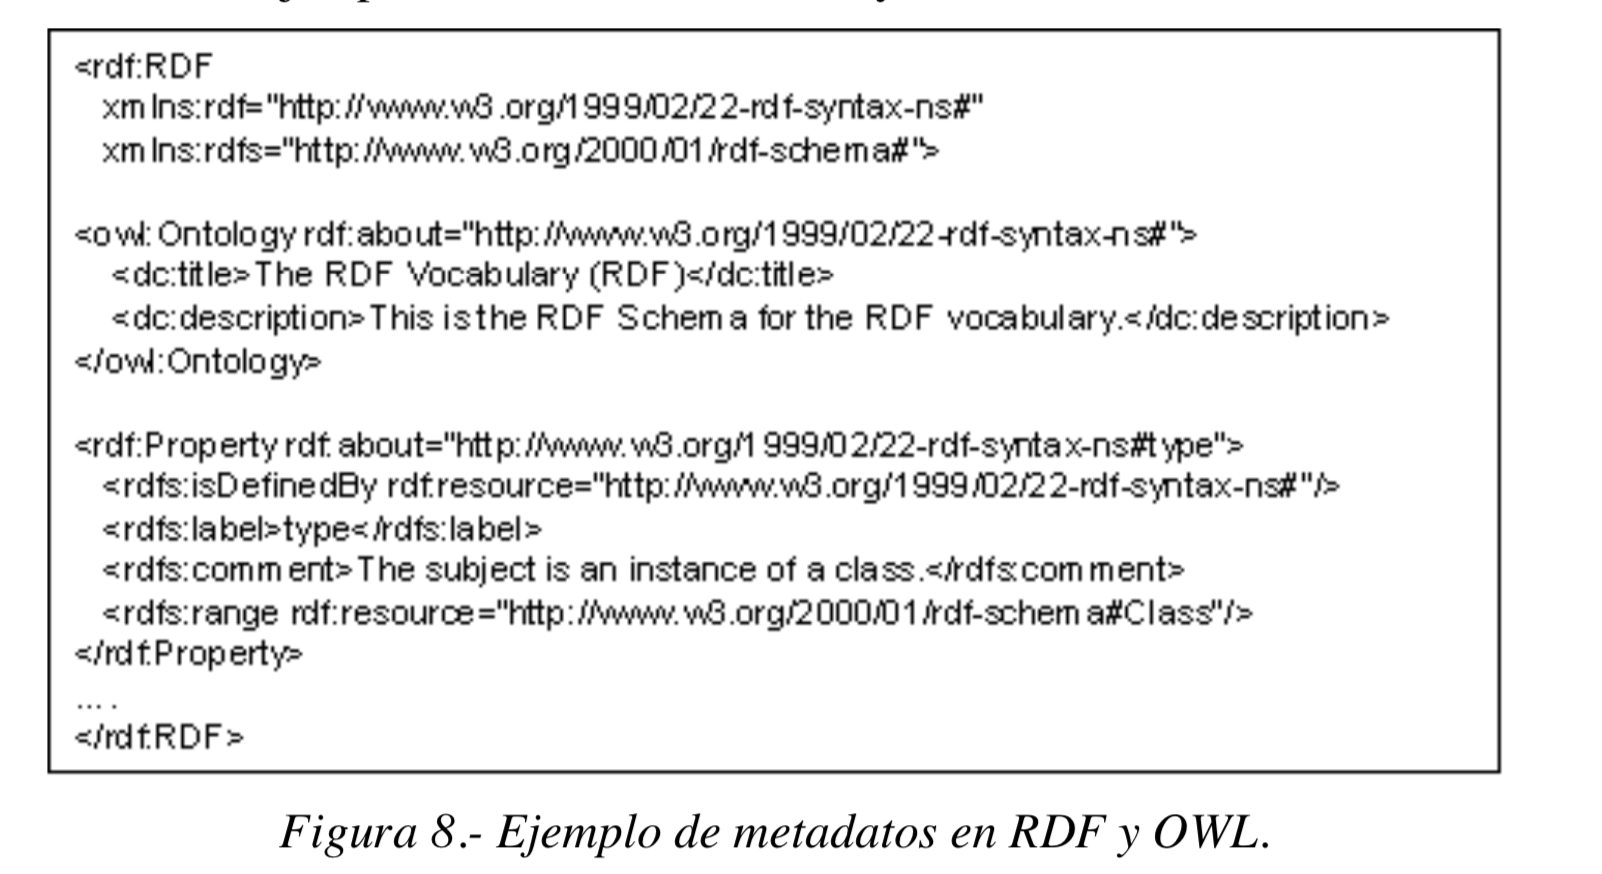
\includegraphics[height=4.5cm]{imagenes/capitulo3/26} % Esquema de los estándares de la Web Semántica
	\caption{}
	\label{}
\end{figure}

% https://www.researchgate.net/publication/216537707_La_Web_semantica_y_las_tecnologias_del_lenguaje_humano
Las dos últimas capas aún no se encuentran integradas en el sistema, pero si el proyecto de la web semántica avanza es previsible que sean las más rápidas en implantarse, ya que la confianza y la seguridad son los elementos clave para dar un paso más allá en el comercio electrónico, que sería uno de los principales motores de la web semántica.

% RESUMEN FINAL DEL APARTADO DE LO QUE ES LA WEB SEMÁNTICA

% https://disenowebakus.net/semantica-web.php
En resumen, podría afirmarse que la Web semántica se enfoca hacia la creación de un espacio compartido para el intercambio de datos altamente estructurados. Se trata de información cuya semántica se presenta de forma que sea relativamente "inteligible" para las aplicaciones. Uno de los aspectos más interesantes de la Web semántica, en el que coinciden la mayoría de los autores, es que, entre otros usos posibles, facilita nuevas posibilidades de comunicación entre hombres y sistemas informáticos a través de servicios que aúnan múltiples fuentes de datos que son tratados para su procesamiento o ejecución de búsquedas de información. De este modo no es necesario duplicar información: Las fuentes de datos se relacionan entre sí sin que importe su ubicación en la Web.

% La Web Semantica y sus Principales Caracteristicas
% https://www.wiziq.com/tutorial/143922-La-Web-Semantica-y-sus-Principales-Caracteristicas

% INTRODUCCIÓN A LA WEB SEMÁNTICA: REALIDADES Y PERSPECTIVAS.
% http://cmap.javeriana.edu.co/servlet/SBReadResourceServlet?rid=1264791321546_232600024_2804

\subsection{De una web de documentos a una web de datos}

% http://www.fgcsic.es/lychnos/es_es/articulos/construyendo_una_web_semantica
Para alcanzar esta visión de una web semántica de entrada no se deberían enlazar únicamente documentos de texto, imágenes u otro contenido multimedia sino directamente los datos sin procesar.

El conjunto de buenas prácticas para la publicación y el enlace de datos estructurados en la Web se conoce como Linked Data, datos enlazados. He aquí sus puntos principales:

% http://www.fgcsic.es/lychnos/es_es/articulos/construyendo_una_web_semantica

- Cada dato –o cada recurso, como suele llamarse a la información en la Web– debe tener un identificador único que lo distingue de cualquier otro dato publicable en la Web. Es lo que se conoce como Universal Resource Identifier, o URI. De hecho muchos usuarios de la Web ya estamos familiarizados con lo que es un URI. Por ejemplo, la dirección https://www.cia.gov/library/publications/the-world-factbook/geos/sp.html es el URI que identifica la página web con la información sobre España en el World Factbook. Pero, para enlazar datos, los URI deben identificar no solo a páginas sino a los elementos concretos que componen los datos. Así, pues, para publicar el hecho de que España y Francia compartan frontera debemos tener unos URI que identifiquen «España», «comparte frontera con» y «Francia», respectivamente.

- Al mismo tiempo, estos identificadores deben ser desreferenciables, lo que significa que el identificador del recurso apunta a su vez al lugar en la Web donde podemos acceder al mismo. La desreferencia de un URI (literalmente «deshacer la referencia») se realiza mediante el protocolo HTTP (Hypertext Transfer Protocol) que posibilita los hipervínculos en la Web: cuando pinchamos sobre uno de estos vínculos, el protocolo HTTP toma el URI y a través de él es capaz de acceder al contenido al cual está apuntando. Lo mismo debe ocurrir ahora con los recursos que componen un dato. El URI de «comparte frontera con» deberá poder ser desreferenciado para acceder a la definición de lo que significa esta relación. Ahí entra la semántica: disponer de estas definiciones y poder acceder a ellas.

- Los datos propiamente dichos se deben expresar usando el Resource Description Framework o RDF, un lenguaje para estructurar los datos en enunciados con el simple formato sujeto-predicado-objeto, y que se conoce como triplete. El sujeto y el objeto son recursos identificados mediante un URI, y el predicado es la relación entre estos recursos. Así pues el hecho de que España comparte frontera con Francia se expresaría en forma de triplete RDF de la siguiente manera:

sujeto: %http://www4.wiwiss.fu-berlin.de/factbook/resource/Spain
predicado: %http://www4.wi­wiss.fu-berlin.de/factbook/ns#landboundary
objeto: %http://www4.wiwiss.fu-berlin.de/factbook/resource/France

Hemos usado las URI de la publicación del World Factbook como Linked Data realizada por la Universidad Libre de Berlín. Como se puede observar, en RDF la relación entre sujeto y objeto –el predicado– es a su vez también un recurso con su URI que debe ser desreferenciable. Como hemos dicho anteriormente, es así como accederemos a sus definiciones, especificando por ejemplo que Spain y France son países y que landboundary es la relación de dos países que comparten una frontera. Estas definiciones que aquí hemos expresado en lenguaje natural deberían ser especificadas a su vez como datos publicados en forma de tripletes RDF.

- Finalmente, para poder utilizar todo el potencial que nos ofrece la infraestructura de la Web, los datos de un repositorio o base de datos deberían estar enlazados con datos externos, definidos en otro repositorio o base de datos. Es decir, el sujeto, predicado y objeto de un mismo triplete RDF no tienen por qué estar ubicados, definidos y gestionados en el mismo repositorio de datos, sino que pueden estar distribuidos por la Web.

Publicando los datos directamente en formato RDF, con unos URI desreferenciables que apuntan a definiciones de entidades y sus relaciones, que a su vez se expresan como datos en RDF enlazando así unos datos con otros, es como se añade a la infraestructura tecnológica existente de la Web este nivel, que puede aumentar significativamente su funcionalidad pues permite procesar estos datos y sus relaciones de forma automatizada. Al igual que en la web de documentos, en la web de datos cualquier persona u organización puede publicar datos, del tipo que sea, y definir los vocabularios asociados a recursos y relaciones. Una buena práctica es usar los URI y los vocabularios ya existentes y ampliamente utilizados. A diferencia de la web de documentos, la estructuración de los datos es independiente de su visualización en pantalla para un usuario humano.

\subsection{Web actual vs. Web Semántica} % Apuntes asignatura

La mayoría de los contenidos de la Web actual están diseñados para ser leídos por humanos.

Los ordenadores puede analizar la estructura de las páginas Web y determinar cuál es la cabecera, dónde hay un enlace a otra página, etc.

- No tienen una forma fiable de procesar la semántica de las páginas.

La Web Semántica proporciona estructura al contenido semántico de las páginas Web, para que puedan ser tratadas por máquinas.

– Crea un entorno donde los agentes que vagan de página a página pueden realizar tareas sofisticadas para los usuarios: no sÓlo miran las palabras clave de las páginas, sino que recogen la semántica de los datos.

Todo ello “sin Inteligencia Artificial”, la semántica está en las páginas. 

– Además, las páginas han sido desarrolladas por usuarios “no informáticos”.

% diagrama de web y diagrama de web semántica

% deberíamos de hablar algo sobre la web

% estaría bien decir que signfica semántica por un lado, que signfica sintáctico por otro y así ir uniendo
% búsquedas semánticas, no sólo sintácticas.

% mencionar algo sobre lo de interoperabilidad

% hablar sobre OGC

% hablar sobre HTML y XML

% https://www.researchgate.net/publication/216537707_La_Web_semantica_y_las_tecnologias_del_lenguaje_humano
\begin{figure}[H]
	\centering
	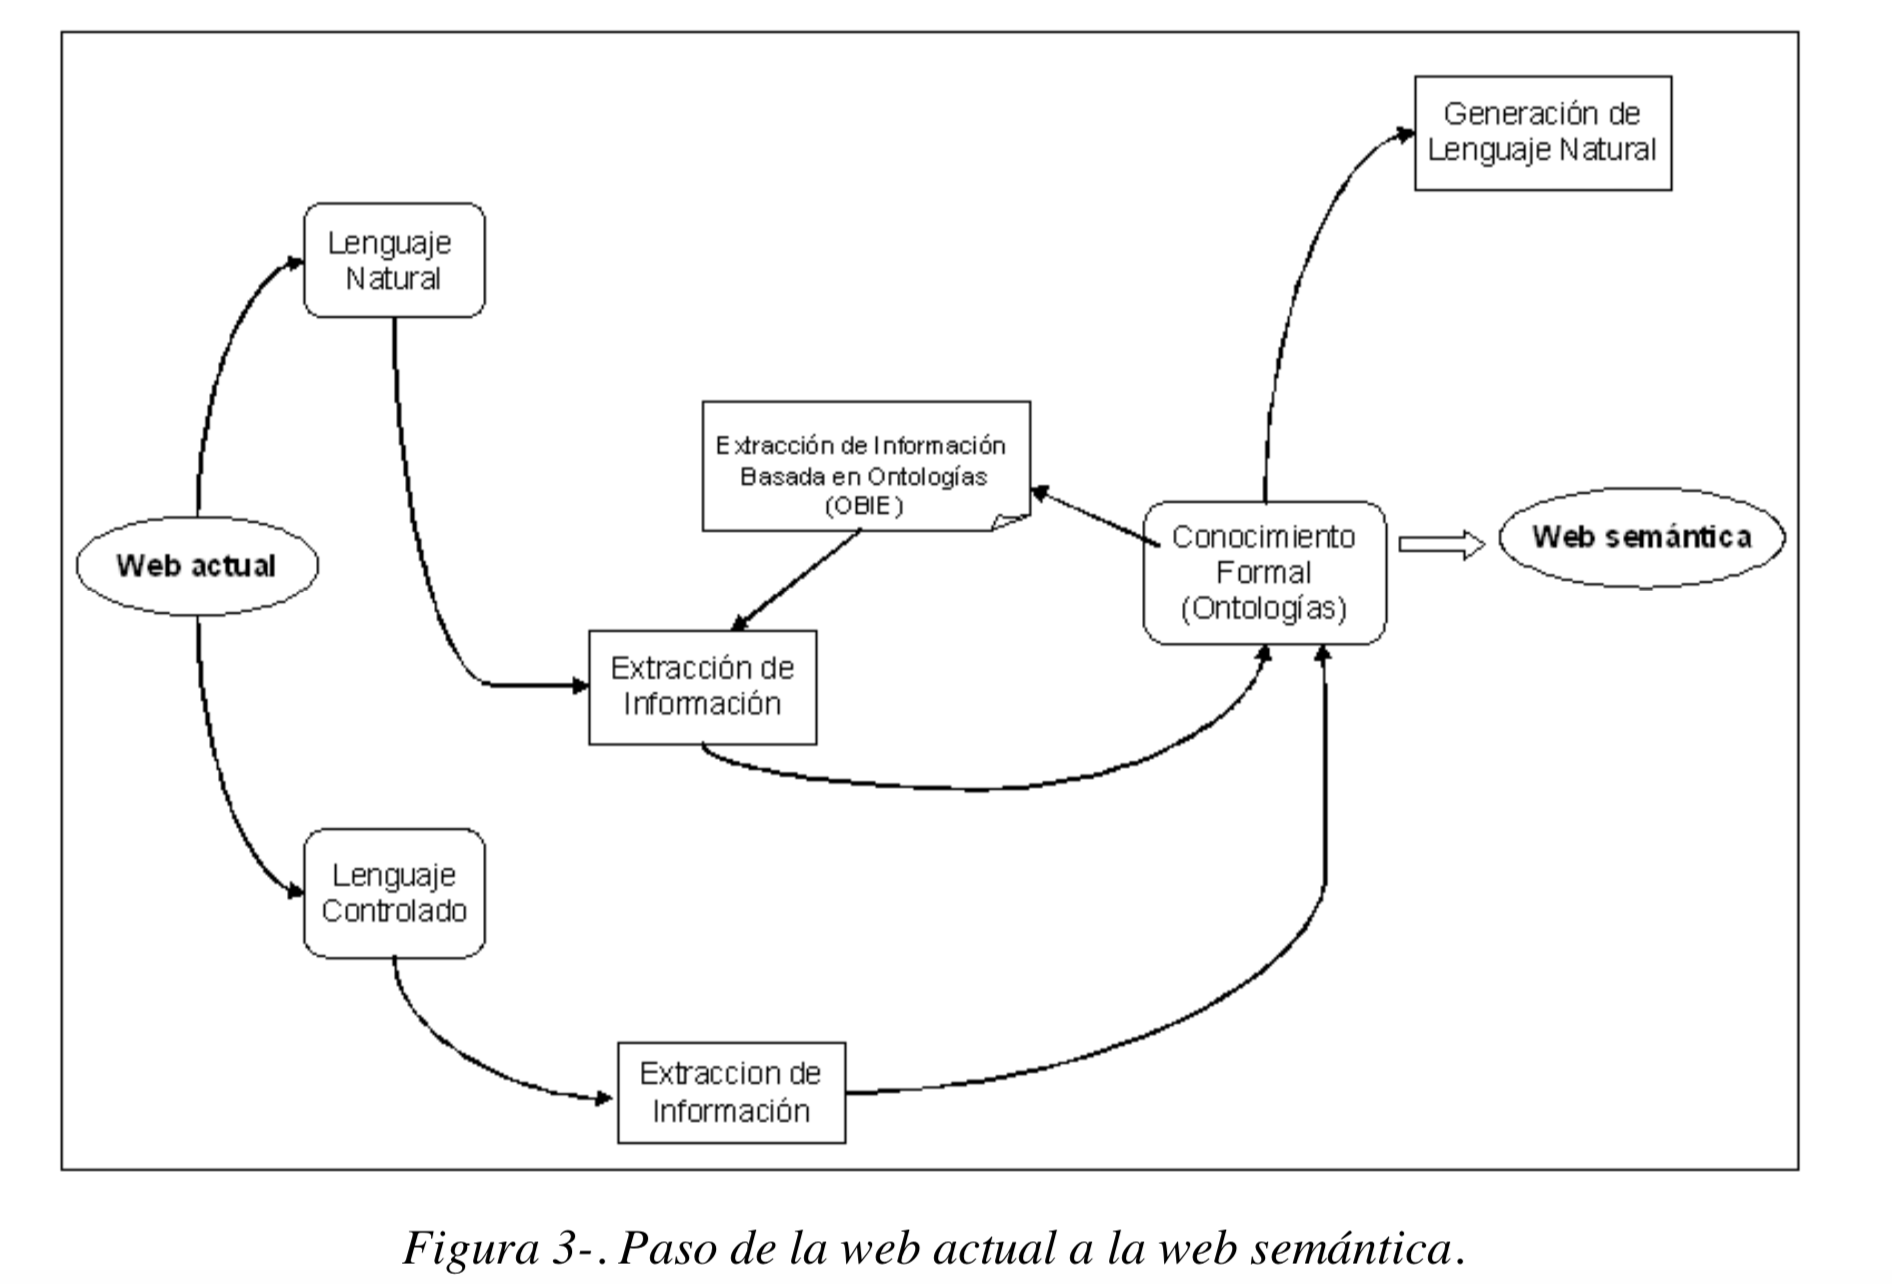
\includegraphics[height=4.5cm]{imagenes/capitulo3/25} 
	\caption{}
	\label{}
\end{figure}

\section{Arquitectura - Estándares de la Web Semántica}

% ARQUITECTURA ESTÁNDARES DE LA WEB SEMÁNTICA

\begin{figure}[H]
	\centering
	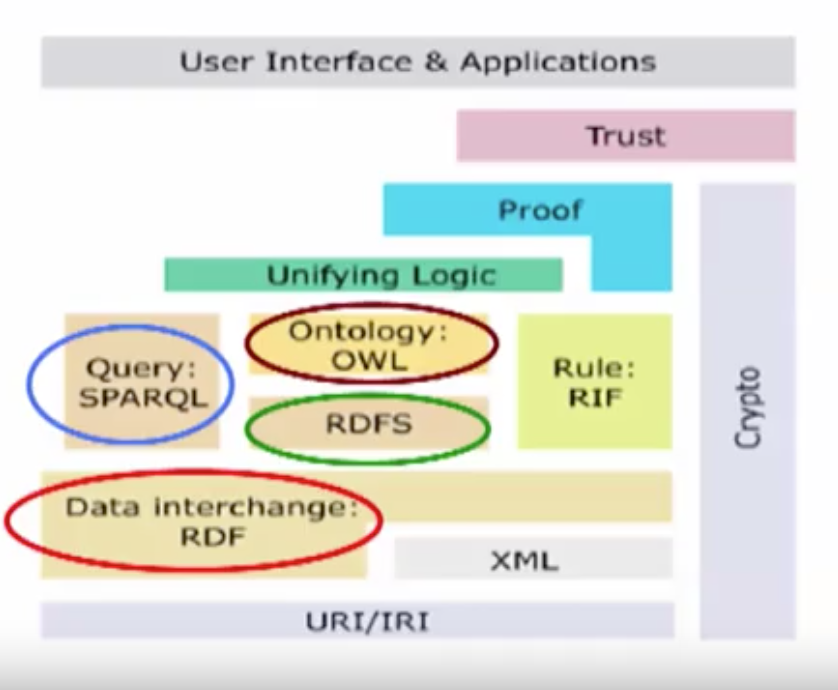
\includegraphics[height=4.5cm]{imagenes/capitulo3/9} % Esquema de los estándares de la Web Semántica
	\caption{}
	\label{}
\end{figure}

% COURSERA: La Web Semántica: Herramientas para la publicación y extracción efectiva de información en la Web
Ahora, ¿cuáles son esos estándares para la web? En la figura usted puede observar la pirámide de estándares que se está desarrollando para llevar a cabo esta web semántica. Y en esta pirámide en la parte inferior vemos los componentes más básicos, en la parte superior donde vemos el trust o el nivel de confianza ve uno en los niveles superiores. En este curso nos vamos a centrar en cuatro de estos componentes de esta pirámide que están marcados con colores. En primer lugar vamos a ver RDF, que es el lenguaje básico para especificar recursos de la web y sus relaciones, RDFS que nos permite decir un poco más vamos a hablar de este vocabulario, SPARQL que es este lenguaje de consulta que nos permite extraer información desde la web y finalmente OWL o este lenguaje que nos permite identificar ontologías. En resumen, ¿qué hemos visto hoy? Hemos visto que hay datos de todo tipo en la web, que son fácil acceso para las personas. Hemos visto que la cantidad de datos es tan grande que las personas no lo pueden manejar en su totalidad, son demasiados para que una persona simplemente pueda procesarlos por sí sola. También hemos visto que es difícil para un computador acceder a estos datos ya que no sabe como interpretarlos. La web de hoy en día está diseñada para ser leídas por personas, las páginas web están diseñadas para ser leídas por personas. ¿Sí? Y no está diseñada para que un computador las pueda leer de manera automática. Y finalmente la web semántica, que es el tema de este curso hemos visto que es un conjunto de recomendaciones para facilitar el acceso de los computadores a los datos. En particular, lo que queremos en este punto es tener el lenguaje que nos permita especificar los recursos que tenemos en la web, especificar las relaciones que tenemos entre ellos y también definir lenguajes que nos permitan extraer de manera automática de esta web.

\begin{figure}[H]
	\centering
	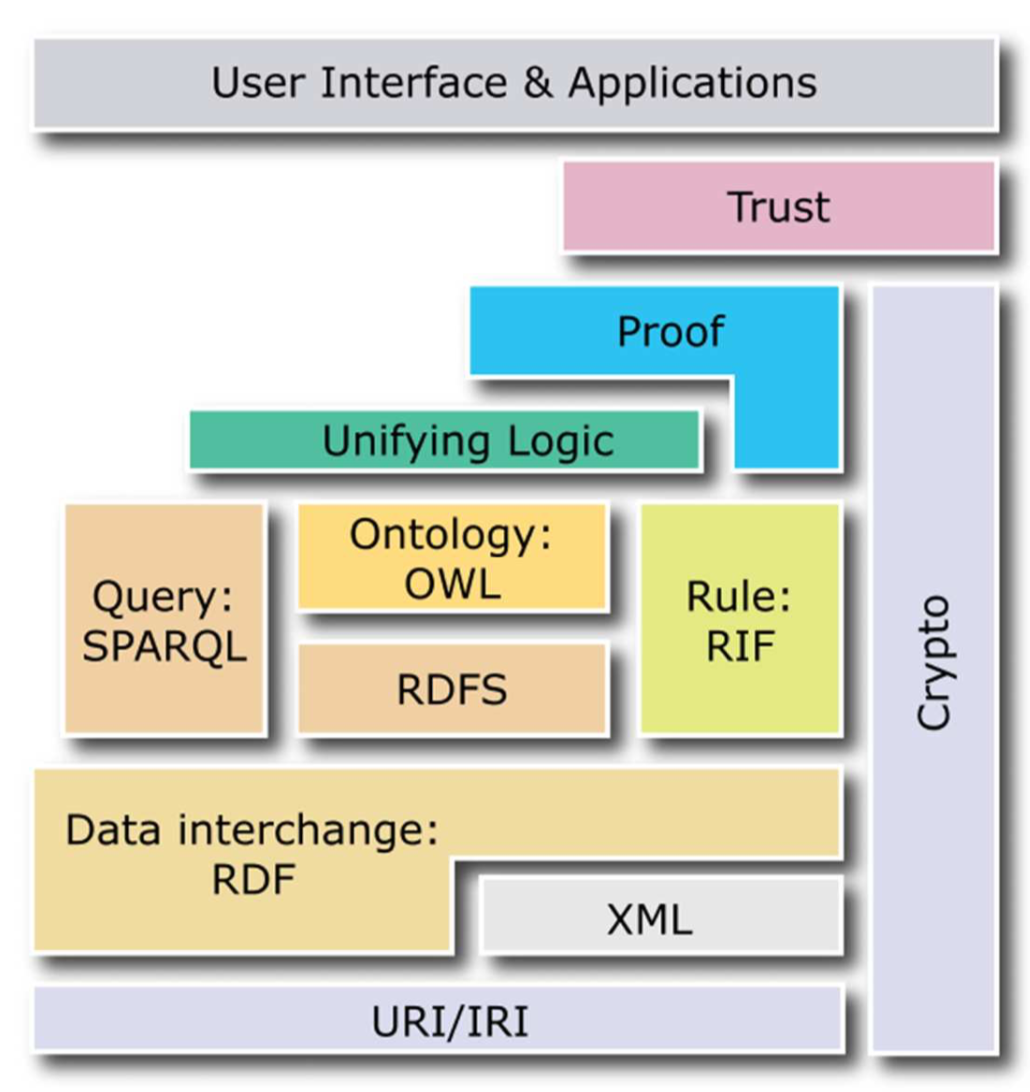
\includegraphics[height=4.5cm]{imagenes/capitulo3/11} % Esquema de los estándares de la Web Semántica
	\caption{}
	\label{}
\end{figure}

\subsection{URI/IRI}

% COURSERA: La Web Semántica: Herramientas para la publicación y extracción efectiva de información en la Web
Antes de continuar, quiero detenerme un momento para describir lo que es una abreviación de URIs. Las URIs normalmente se abrevian poniendo al principio del archivo prefix dbpedia y la base de la URI, http://dbpedia.org/resource como vemos en este ejemplo. Entonces más adelante, simplemente ponemos dbpedia:Lionel_Messi y podemos acceder al recurso identificado por la URI completa, es decir por http://dpbedia.org/resource/Lionel_Messi

\begin{figure}[H]
	\centering
	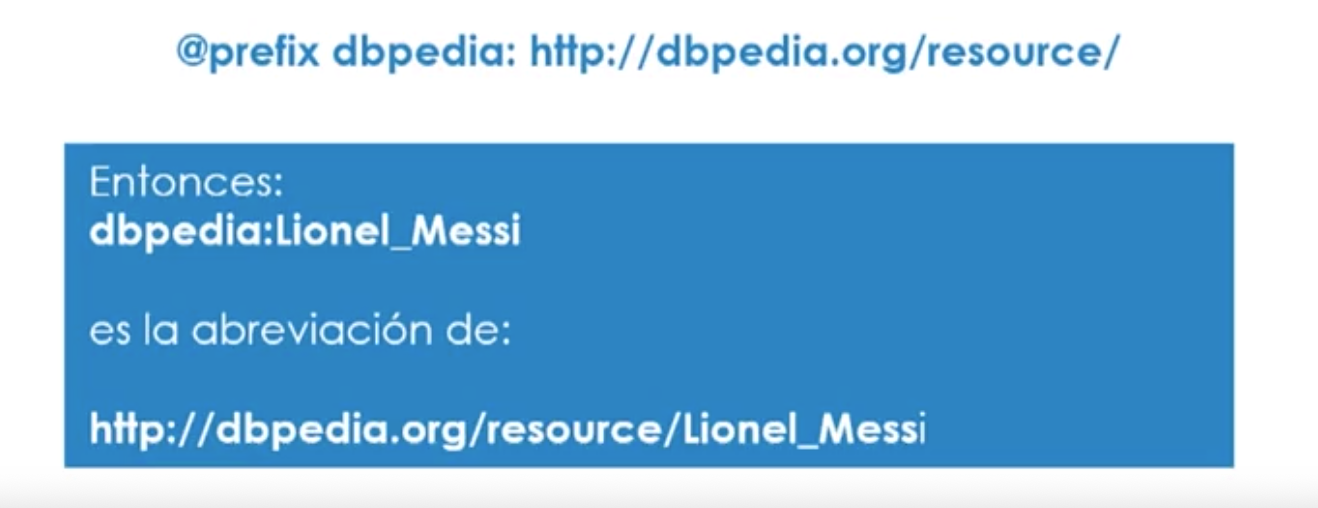
\includegraphics[height=4.5cm]{imagenes/capitulo3/13} 
	\caption{}
	\label{}
\end{figure}

\subsection{XML}

% Libro Geospatial Semantic Web
Geography Markup Language (GML) es “una gramática XML escrita en XML Schema para el modelado, transporte y almacenamiento de información geográfica, incluidas las propiedades espaciales y no espaciales de las características geográficas”

% Hablar que hay un problema con HTML y surge el poder el XML

\subsection{RDF}

%  Lo que XML nos ofrece y de lo que carece

\subsubsection{Las nociones de literal y triple RDF}

% COURSERA: La Web Semántica: Herramientas para la publicación y extracción efectiva de información en la Web
Hoy, lo que vamos a hacer es ver los conceptos clave de la web semántica. Uno es el concepto de literal en RDF y otro es el concepto de triple RDF.

% COURSERA: La Web Semántica: Herramientas para la publicación y extracción efectiva de información en la Web
Primero, ¿qué es un literal? Un literal lo que hace es representar un valor concreto en una especificación RDF. Por ejemplo, Messi nació en la fecha 1987-06-24. Esto es un literal y está encerrado entre comillas. Otros ejemplos de literales son 1987-06, Lionel Messi, 169.03, 18:25:00. Todos estos son literales y son cadenas de caracteres que van encerrados entre comillas.

% COURSERA: La Web Semántica: Herramientas para la publicación y extracción efectiva de información en la Web
Un literal, además, puede tener un tipo asociado. En los siguientes literales, los tipos destacados en rojo son los tipos de los literales. Por ejemplo, una fecha entre comillas 19877-06-24 xsd:date indica que es una fecha. El literal, lo que está encerrado entrecomillas es una fecha. Si no estuviese este xsd:date no sería una fecha. Simplementes sería una cadena de caracteres un literal normal y corriente. Después tenemos que para indicar que un número es un número real. Por ejemplo 169.03 añadimos al final que es un xsd:float.

% COURSERA: La Web Semántica: Herramientas para la publicación y extracción efectiva de información en la Web
De la misma forma, para indicar que un literal es de tipo tiempo, time, hora añadimos al final de la cadena de caracteres xsd time. Esto es importante porque así una aplicación, cuando lee un documento sabe que cada cadena de caracteres, cada literal, es de un determinado tipo. Y así puede identificar, por ejemplo una fecha de nacimiento, una altura, la hora etcétera. Otros ejemplos de literales son 1987-06-24 entre comillas pero sin ningún tipo asociado esto es simplemente una cadena de caracteres. Si le añadimos xsd:date es de tipo fecha. 169.03 entre comillas es una cadena de caracteres. Y si le añadimos a 18:25:00 xsd:time entonces es la hora. Y así una aplicación puede interpretar correctamente los datos que está leyendo.

\begin{figure}[H]
	\centering
	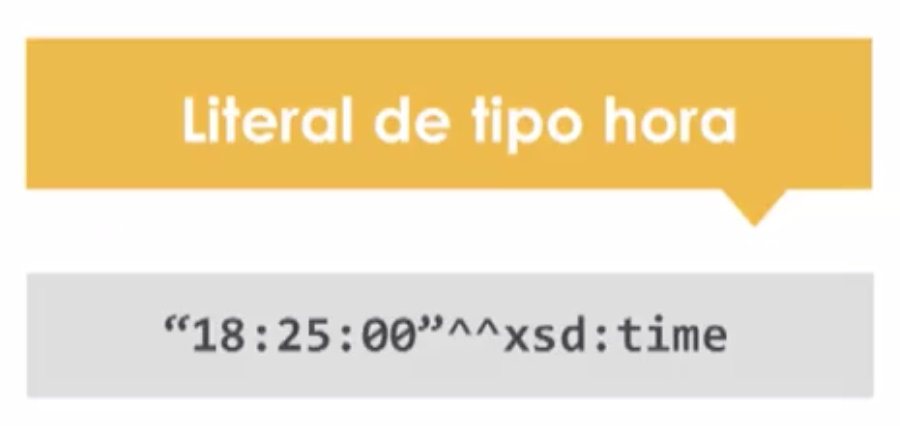
\includegraphics[height=4.5cm]{imagenes/capitulo3/12} 
	\caption{}
	\label{}
\end{figure}

% COURSERA: La Web Semántica: Herramientas para la publicación y extracción efectiva de información en la Web
Ahora que ya conocemos los elementos básicos de RDF vamos a describir las relaciones que podemos construir utilizando estos elementos básicos. Lo primero que debemos entender y tener muy claro es el concepto de triple. Un triple especifica la relación entre dos recursos, o se utiliza para dar valor a un atributo de un recurso.

% COURSERA: La Web Semántica: Herramientas para la publicación y extracción efectiva de información en la Web
Por ejemplo, un triple está formado por sujeto, predicado, y objeto. El sujeto se identifica por una URI. Es el recurso identificado por una URI. El predicado también utiliza una URI la cual representa la relación entre recursos o los atributos que va a tener el sujeto anterior. Y finalmente, el objeto lo que hace es identificar o bien el recurso que es el objeto de la relación o el valor del atributo especificado en la relación.

% COURSERA: La Web Semántica: Herramientas para la publicación y extracción efectiva de información en la Web
Unos ejemplos de triples RDF son los siguientes. Dbpprop identifica la URI de las propiedades en DBpedia. Dbpedia: dbpedia.resource identifica los recursos que existen en DBpedia como, por ejemplo, Lionel Messi. Example: example.org identifica abrevia la URI example.org. Y el prefijo dos puntos, que también se puede poner dos puntos sin ningún tipo de nombre es la abreviación para la URI ejemplo.org.

\begin{figure}[H]
	\centering
	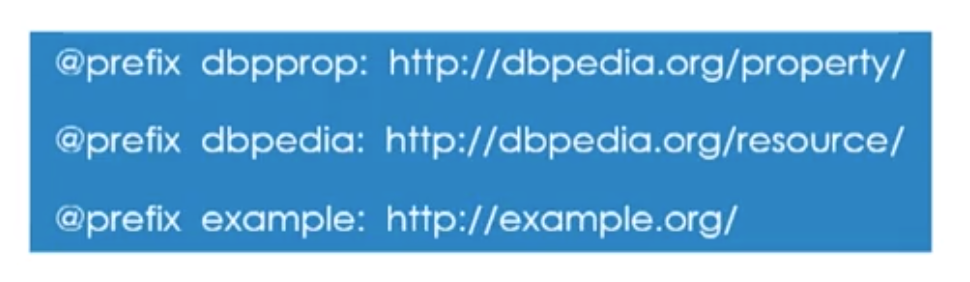
\includegraphics[height=4.5cm]{imagenes/capitulo3/14} 
	\caption{}
	\label{}
\end{figure}

% COURSERA: La Web Semántica: Herramientas para la publicación y extracción efectiva de información en la Web
Una vez que tenemos esto claro ya podemos continuar con el siguiente ejemplo. Este ejemplo indica que dbpedia dos puntos Lionel_Messi, es decir el recurso identificado por la URI de Lionel Messi tiene la propiedad nació, o lugar de nacimiento en dbpedia:Argentina. Este triple lo que hace es indicar la relación entre los recursos Lionel Messi y Argentina, y esa relación es que nació en. Lionel Messi nació en Argentina.

\begin{figure}[H]
	\centering
	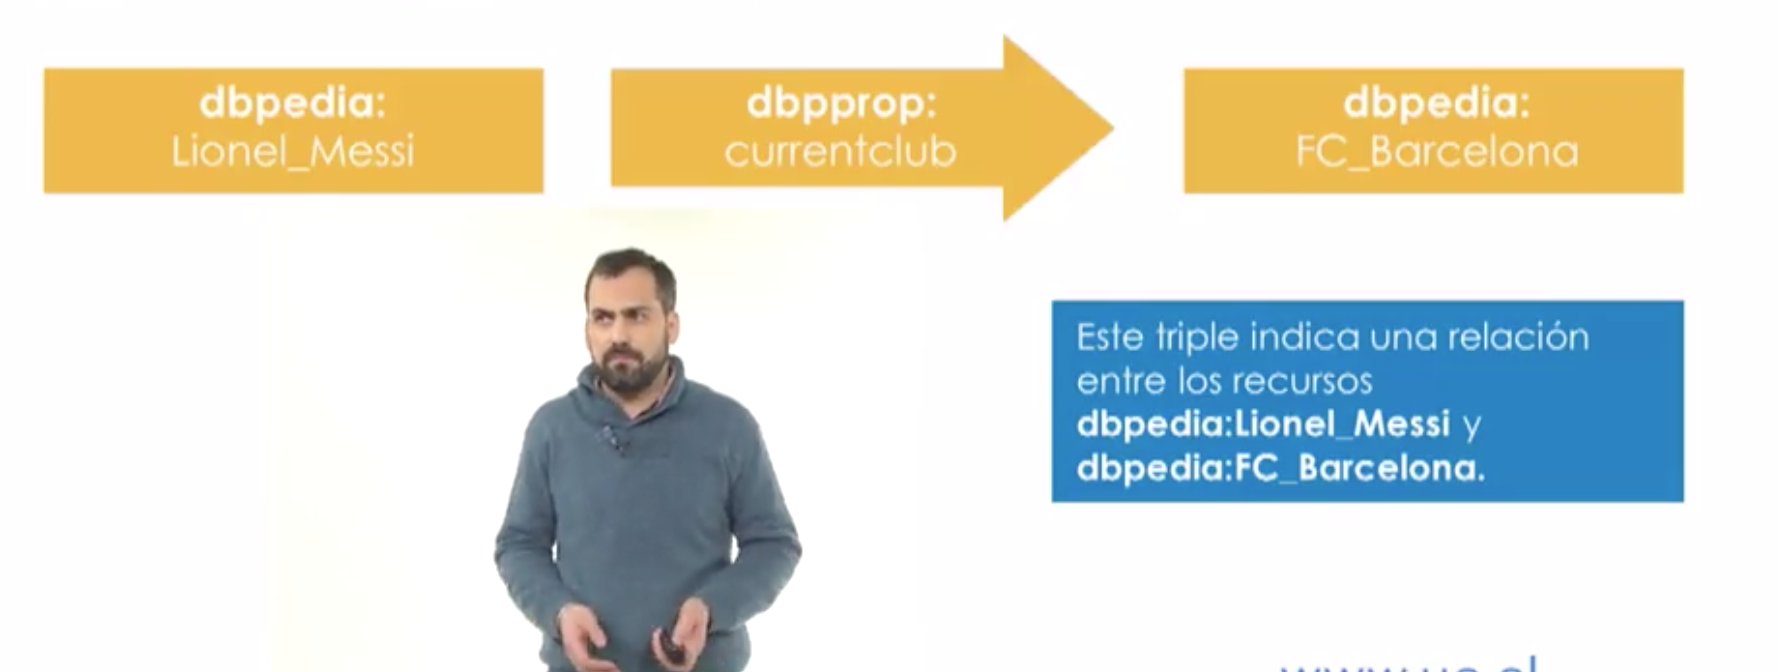
\includegraphics[height=4.5cm]{imagenes/capitulo3/15} 
	\caption{}
	\label{}
\end{figure}

% COURSERA: La Web Semántica: Herramientas para la publicación y extracción efectiva de información en la Web
Otro ejemplo de triple es, por ejemplo dbpedia:Lionel_Messi, currentclub el club en el que juega actualmente es el fútbol club Barcelona. Este triple indica que Messi juega en el Barcelona.

% COURSERA: La Web Semántica: Herramientas para la publicación y extracción efectiva de información en la Web
Y un tercer ejemplo de triple, en el sujeto tenemos Lionel Messi. La relación example:birthday, nosotros definimos la relación que va a cumplir Messi. Y el atributo 1987-06 -24. Entonces, este ejemplo lo que hace es indicar que el valor del atributo que Messi tiene una relación o un atributo que es ejemplo:birthday. Y el valor es 1987-06-24. Hay que tener en cuenta de que esto no indica que sea una fecha. Simplemente es una cadena de caracteres.

% COURSERA: La Web Semántica: Herramientas para la publicación y extracción efectiva de información en la Web
Entonces, ¿qué hemos aprendido en este módulo? Primero, sabemos lo que es un literal. Que puede tener tipo o no, y esto es importante para que los programas, el software sea capaz de identificar correctamente o interpretar correctamente los datos que lee. Después hemos definido lo que es un triple RDF. Un triple RDF está compuesto por sujeto que es un recurso, una URI. Un predicado, que es una URI que indica la relación de ese recurso con el objeto que es o bien una URI o bien un valor para un atributo.

\subsubsection{El concepto de grafo RDF}

% COURSERA: La Web Semántica: Herramientas para la publicación y extracción efectiva de información en la Web
Continuando con el estudio de las nociones básicas y del modelo de datos RDF hoy vamos a ver el concepto de grafo RDF. ¿Qué es un grafo RDF? Bueno, un grafo RDF es simplemente un conjunto de triples RDF. Por ejemplo, puede ver en esta figura, un grafo RDF que está formado por un triple RDF y en este triple RDF especificamos que Lionel Messi, nació en Rosario. Recuerde que en el triple RDF está formado por un sujeto, un predicado y un objeto, y en estos tres componentes usamos URIs, una URI es una dirección, un identificador de un recurso en la web. Por ejemplo, el URI dbpedia Lionel Messi es un URI que identifica el rescurso de Lionel Messi. El URI dbprop birth place es un URI que identifica a esta propiedad que es el lugar de nacimiento y dbpedia Rosario es un URI que identifica la ciudad de Rosario, en Argentina. Además, note que en estos URIs estamos usando prefijos, estos prefijos nos ayudan a simplificar la anotación, vamos a ver en nuestras pasos siguientes cuáles son estos prefijos. 

\begin{figure}[H]
	\centering
	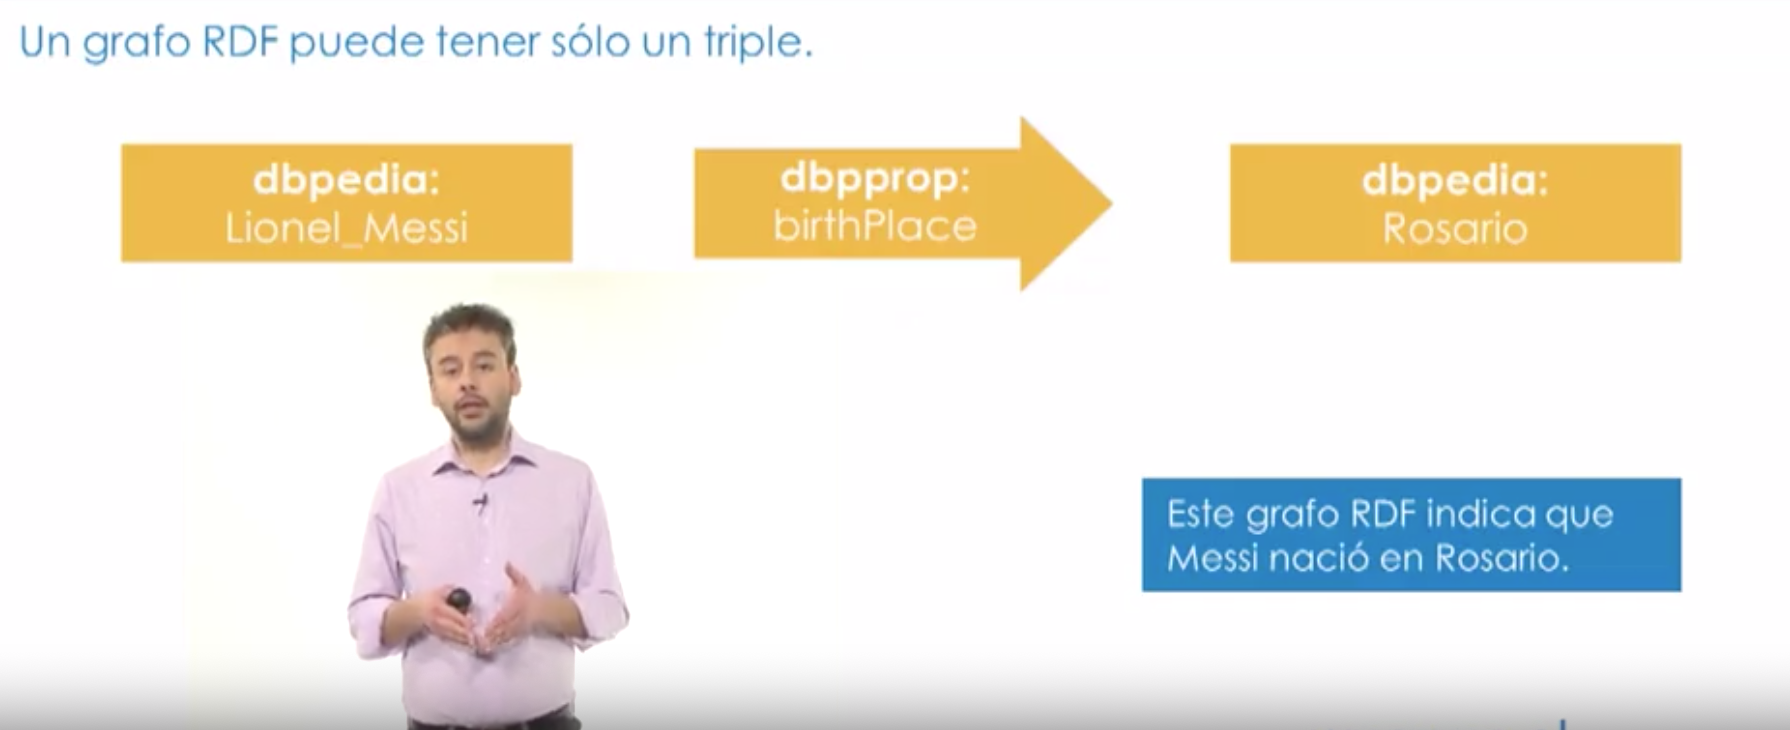
\includegraphics[height=4.5cm]{imagenes/capitulo3/16} 
	\caption{}
	\label{}
\end{figure}

% COURSERA: La Web Semántica: Herramientas para la publicación y extracción efectiva de información en la Web
Podemos encontrar ejemplos con más triples. En este tercer ejemplo, tenemos un grafo RDF más complejo. En este caso, tenemos cuatro triples, tenemos los dos triples anteriores pero además decimos en este grafo RDF que Rosario es parte de la provincia de Santa Fé. Nótese que en este caso estamos usando el triple que dice dbpedia Rosario, dbprop is part of al dbpedia Santa Fé Province. Estamos diciendo entonces que Rosario es parte de esta provincia. Y también tenemos un triple que nos dice que, el Barcelona es parte de la provincia de Barcelona. Nuevamente importante esta destacar acá que en este triple estamos usando un URI dbpedia Barcelona para identificar a la ciudad de Barcelona, dbprop is part of para identificar esta propiedad que nos dice, que, identifica, para una ciudad, eh, la provincia de la cuál es parte de, y además tenemos dbpedia Province of Barcelona que es un URI que nos indica, que identifica a la provincia de Barcelona, en España.

\begin{figure}[H]
	\centering
	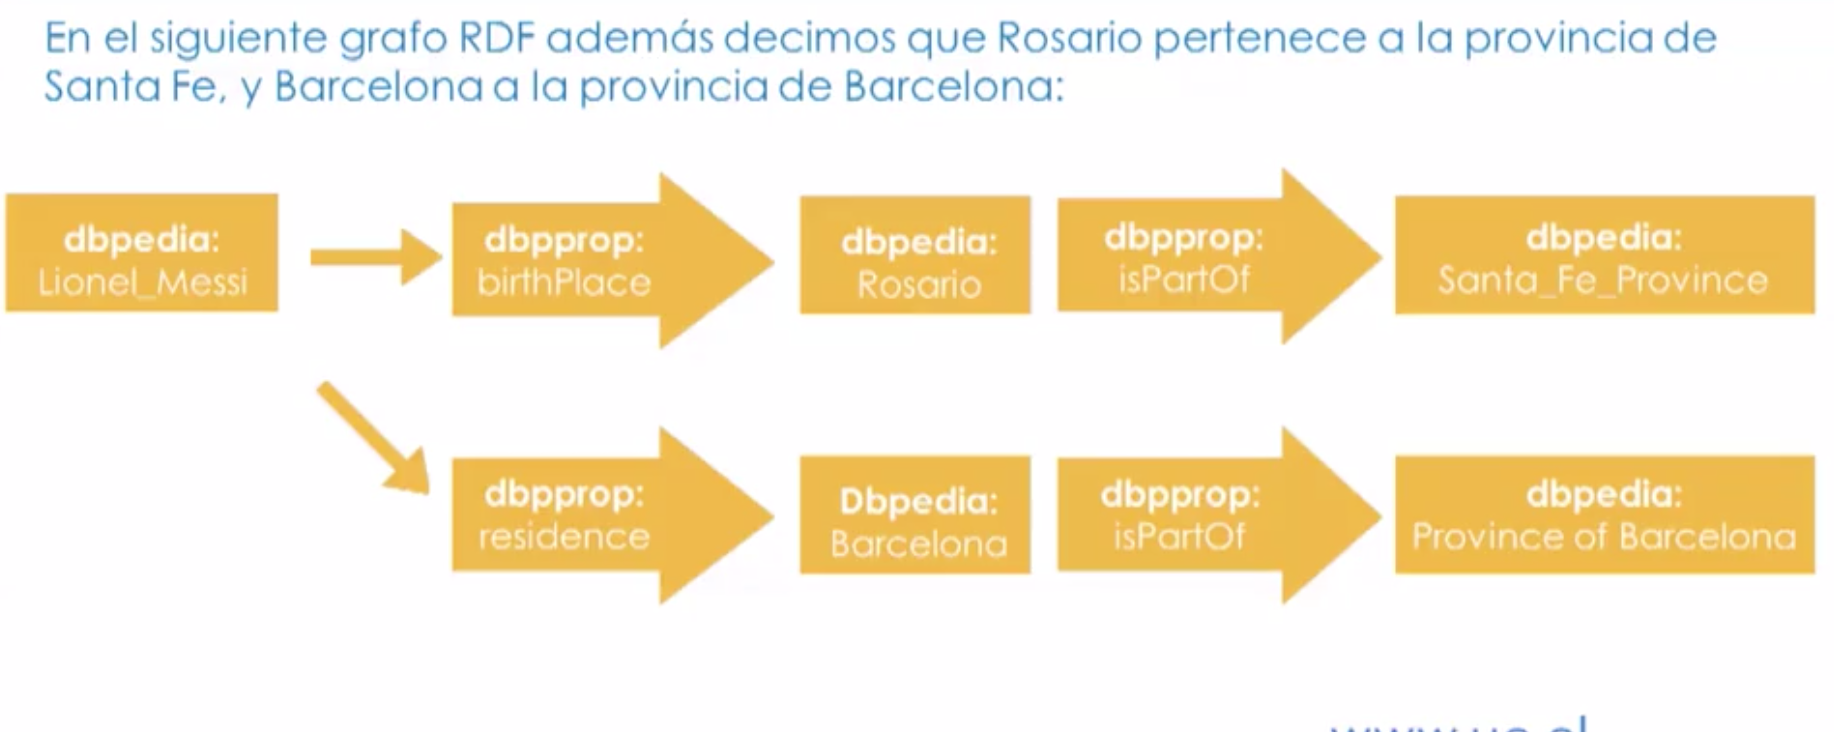
\includegraphics[height=4.5cm]{imagenes/capitulo3/17} 
	\caption{}
	\label{}
\end{figure}

% COURSERA: La Web Semántica: Herramientas para la publicación y extracción efectiva de información en la Web
Ahora, ¿cómo se vé un grafo RDF en la web? Lo que hemos construido hasta ahora, es un grafo que está constituido por triples. En estos triples, tenemos, por ejemplo, indicamos que Messi nació en Rosario, que Messi vive en Barcelona, que Rosario es parte de la provincia de Santa Fé y que Barcelona es parte de la provincia de Barcelona. Ahora, pero ¿cómo se almacena este grafo en la web? Bueno, este grafo es simplemente, es almacenado como un conjunto de triples. Lo que vemos en esta figura, es un archivo donde tenemos cuatro triples y esta es la forma en la cual, uno lo escribiría, en la web. Nos dice que, el primer triple nos indica que Lionel Messi, nació en Rosario y que usamos el punto para indicar cuándo un triple, el punto de término de un triple, ¿sí? Entonces en este caso, tenemos un primer triple, Lionel Messi nació en Rosario, punto. Un segundo triple que nos dice, Lionel Messi tiene como residencia a Barcelona, punto.

\begin{figure}[H]
	\centering
	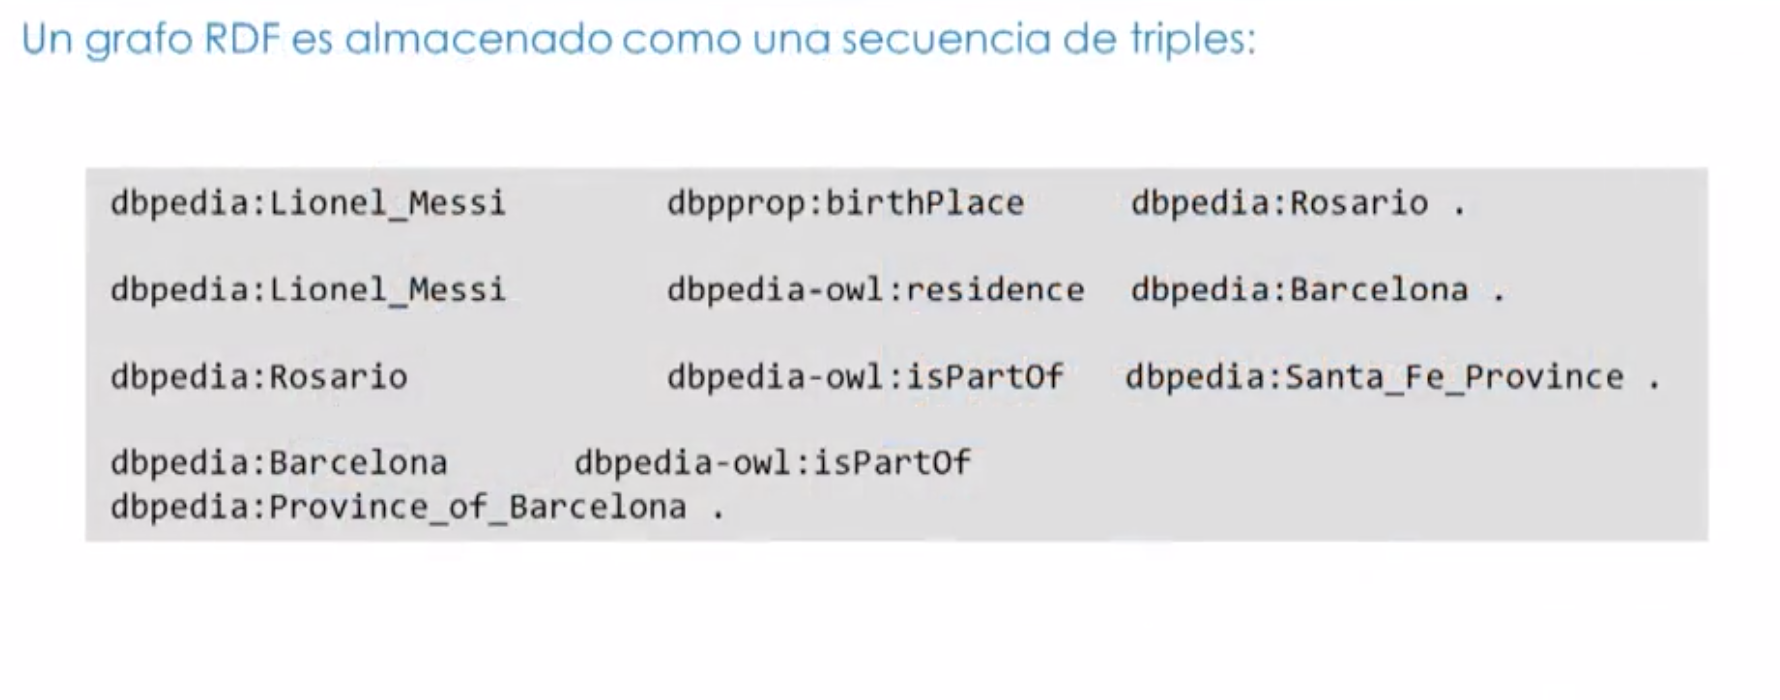
\includegraphics[height=4.5cm]{imagenes/capitulo3/18} 
	\caption{}
	\label{}
\end{figure}

% COURSERA: La Web Semántica: Herramientas para la publicación y extracción efectiva de información en la Web
Ahora, cómo lo habíamos mencionado anteriormente, en cada uno de estos triples, estamos usando URIs, en cada uno de estos URIs estamos usando prefijos que nos ayudan a simplificar la anotación de los URIs. En los grafos anteriores hemos usado estos prefijos. O sea por ejemplo, tenemos dbpedia que corresponde a este URI que es mencionado en la transparencia, que es http:dbpedia.org/resource. Entonces, cuando miramos el grafo completo RDF lo que vamos a ver es algo como lo siguiente, en primer lugar, especificamos los prefijos, indicamos, estos son los prefijos que estamos usando en el archivo RDF. El primer prefijo es el prefijo para dbpedia, el segundo es para dbprop y el tercero es para dbpedia owl y y a continuación especificamos cuales son los triples que tenemos en nuestro grafo. Por ejemplo, dbpedia:Lionel Messi y dbpedia prop: birthplace, dbpedia:Rosario. Ese es el primer triple que nos indica que Lionel Messi nació en Rosario. Y nótese que, si uno quiere construir el URI que representa a Lionel Messi, lo que tiene que hacer, como habíamos explicado anteriormente es tomar el prefijo dbpedia y reemplazarlo y al hacer eso, lo que obtenemos es el URI para Lionel Messi que en este caso es, http:dbpedia.org/resource/Lionel Messi. Entonces, como resumen de nuestro video lo que hemos visto es que un grafo RDF está formado por un conjunto de triples RDF, un grafo RDF en la web se almacena como una secuencia de triples y usamos el punto para indicar cuando un triple termina. En cada uno de estos triples es importante recordar que, tenemos un sujeto, un objeto y un, un sujeto, un predicado y un objeto y que para representar estos elementos, utilizamos un URIs y en general, para simplificar la escritura de los URIs, lo que utilizamos en los grafos RDF son abreviaciones y estas abreviaciones son especificadas al principio de un archivo RDF. 

\begin{figure}[H]
	\centering
	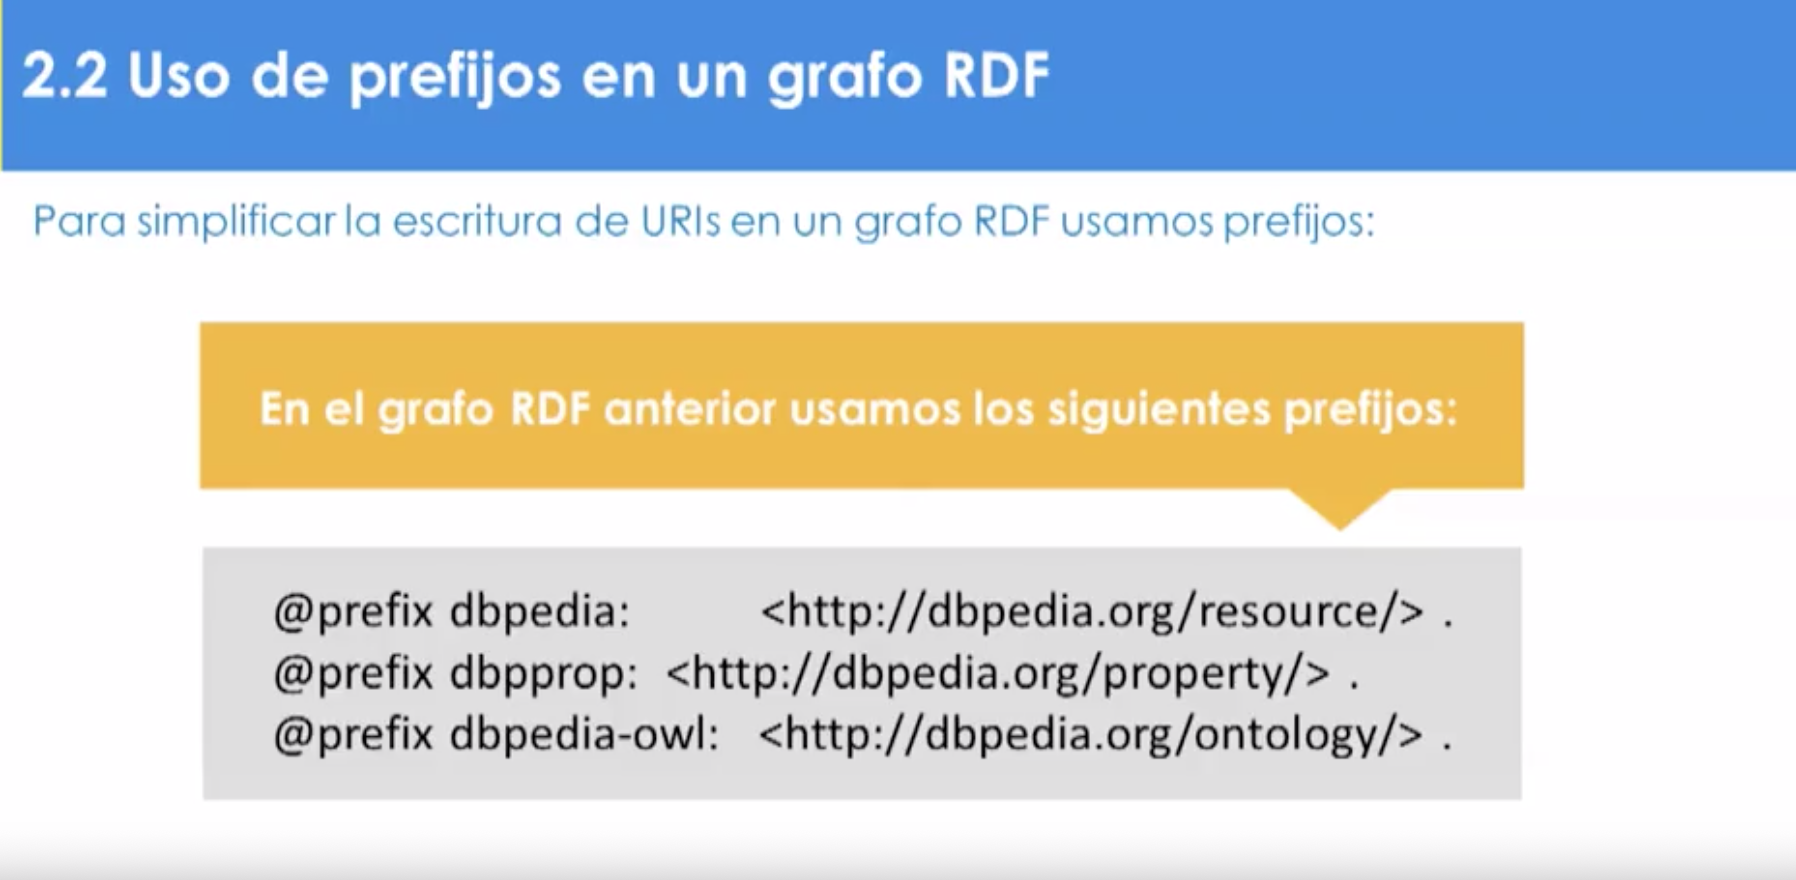
\includegraphics[height=4.5cm]{imagenes/capitulo3/19} 
	\caption{}
	\label{}
\end{figure}

\subsubsection{Vocabularios RDF} % Hoy lo que vamos a ver son Vocabularios RDF.

% COURSERA: La Web Semántica: Herramientas para la publicación y extracción efectiva de información en la Web
Llegados a este punto, quizá se pregunten, ¿cómo pueden dos aplicaciones distintas entenderse entre ellas? Bien, esta pregunta es similar a la de, ¿cómo dos personas distintas pueden entenderse entre ellas?

% COURSERA: La Web Semántica: Herramientas para la publicación y extracción efectiva de información en la Web
La respuesta es porque utilizan no solo el mismo lenguaje, sino también las mismas palabras para nombrar a las cosas a las que se refieren, es decir, utilizan el mismo vocabulario. Entonces, ahora vamos a mostrar lo que son los vocabularios dentro de RDF que es el lenguaje de la Web Semántica.

\begin{figure}[H]
	\centering
	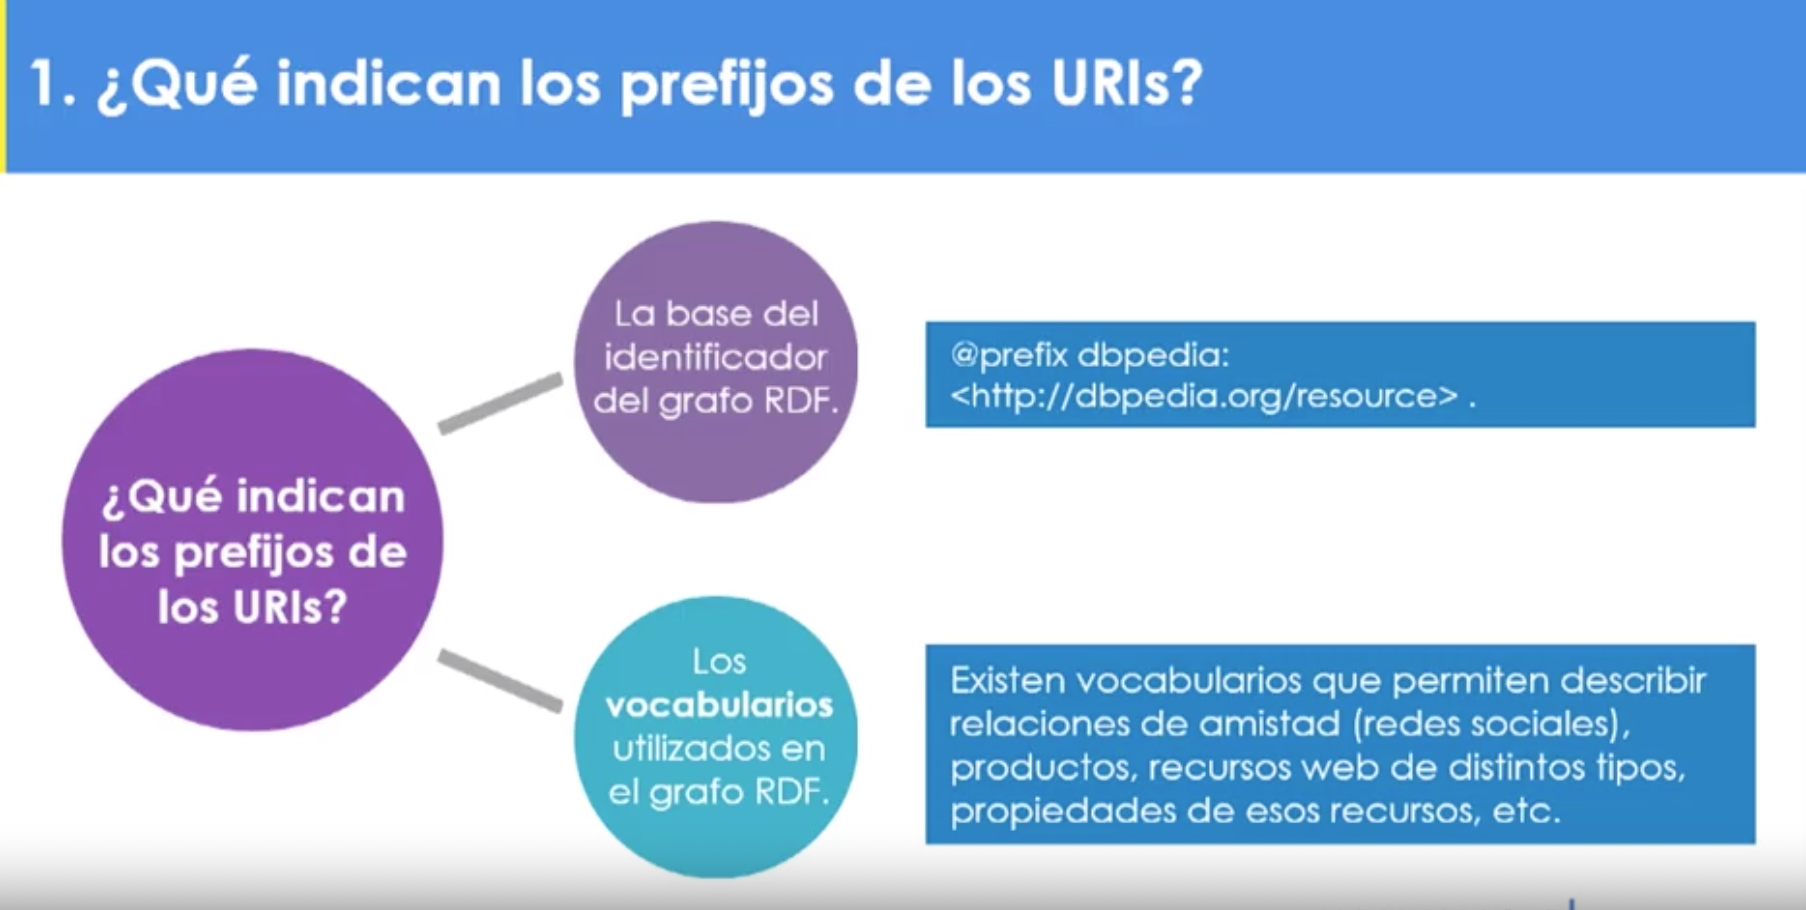
\includegraphics[height=4.5cm]{imagenes/capitulo3/20} 
	\caption{}
	\label{}
\end{figure}

% COURSERA: La Web Semántica: Herramientas para la publicación y extracción efectiva de información en la Web
Primero, los prefijos en la URIs no solo se utilizan para abreviar una URI, también se utilizan como vocabulario que se va a utilizar dentro de los datos, es decir, hay vocabularios que describen productos, relaciones de amistad, autos. Hay una gran cantidad de vocabularios y todos se intentan utilizar de la misma forma a la hora de generar datos RDF.

% COURSERA: La Web Semántica: Herramientas para la publicación y extracción efectiva de información en la Web
Por ejemplo, los vocabularios que sirven como vocabulario común para nombrar y describir recursos en la web, se utilizan en distintas bases de datos. Un ejemplo es la de DBpedia en inglés, utiliza la propiedad birthPlace como nombre, como vocabulario, como predicado para indicar que un lugar es un lugar de nacimiento, que una persona nació en un lugar determinado.

% COURSERA: La Web Semántica: Herramientas para la publicación y extracción efectiva de información en la Web
En otra base de datos distinta, otra base de datos RDF distinta, como es la Dbpedia en español, no es tan distinta pero están relacionadas.

% COURSERA: La Web Semántica: Herramientas para la publicación y extracción efectiva de información en la Web
Es utilizada en la misma propiedad para indicar que una persona nació en un lugar. Así pues, utiliza el mismo vocabulario La Dbpedia en español utiliza el mismo vocabulario que la DBpedia en inglés para describir las propiedades que un recurso puede tener.

% COURSERA: La Web Semántica: Herramientas para la publicación y extracción efectiva de información en la Web
En resumen, los vocabularios sirven para construir un lenguaje común y estándar para todos. Es básicamente como intentar construir la Torre de Babel otra vez.

% COURSERA: La Web Semántica: Herramientas para la publicación y extracción efectiva de información en la Web
Por ejemplo, ahora un ejemplo de vocabulario bastante conocido es FOAF. FOAF significa Friend of a Friend y es un vocabulario para nombrar relaciones entre personas, es un vocabulario de red social, de hecho es el primer vocabulario para redes sociales que existió.

% COURSERA: La Web Semántica: Herramientas para la publicación y extracción efectiva de información en la Web
FOAF contiene elementos como por ejemplo que son agente, persona y tienen un significado unívoco, es decir, en FOAF cuando un recurso es identificado como persona, es una persona. Es decir, Yo, Carlos, está bien si estoy identificado como persona, soy una persona, y eso, una aplicación software es capaz de entenderlo.

% COURSERA: La Web Semántica: Herramientas para la publicación y extracción efectiva de información en la Web
Si en un documento RDF o una página web existe mi recurso y la relación FOAF tipo persona, el software va a saber interpretar que yo soy una persona, ese recurso es una persona. Además, FOAF también puede, también define distintas propiedades que pueden tener las personas como Last Name, Family Name, Fest Name, Nickname, Email, Web Page. Es decir, FOAF es un vocabulario que sirve para describir un recurso, a una persona, de una forma bastante detallada y que una aplicación sea capaz de entender cuando lee ese recurso RDF todas las relaciones que tiene esa persona.

% COURSERA: La Web Semántica: Herramientas para la publicación y extracción efectiva de información en la Web
El siguiente es un archivo de, un archivo FOAF en el cual se describe a Carlos. Es de tipo persona, Carlos, que tiene el nombre Carlos, Carlos que tiene el nombre de familia, Buil de apellido.

\begin{figure}[H]
	\centering
	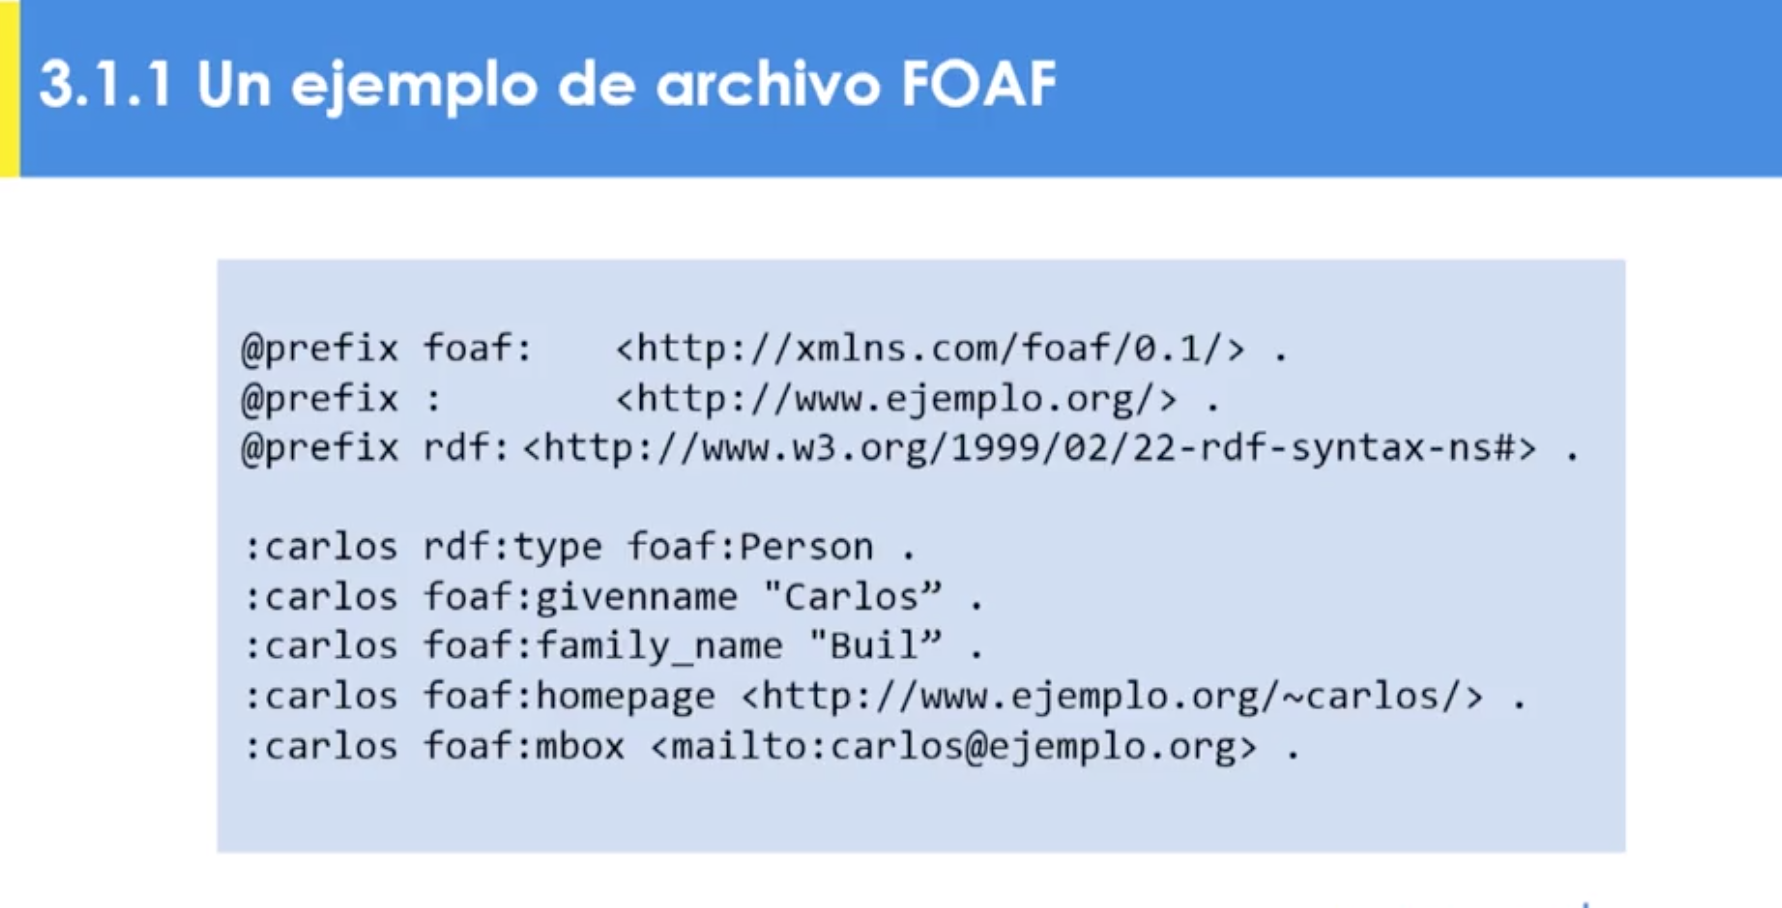
\includegraphics[height=4.5cm]{imagenes/capitulo3/21} 
	\caption{}
	\label{}
\end{figure}

% COURSERA: La Web Semántica: Herramientas para la publicación y extracción efectiva de información en la Web
Carlos que tiene la página web ejemplo.org y tiene el email ejemplo.org. Este es un archivo RDF utilizando el vocabulario FOAF. Entonces, para resumir, hemos visto que los vocabularios son importantes. Los vocabularios son los que nos permiten hablar el mismo lenguaje, Permiten que dos aplicaciones se puedan entender, o que una aplicación pueda genera datos y la otra pueda consumirlos, entendiéndose entre ellos. En la web existen bastantes vocabularios para describir productos, relación de amistad, autos, hay muchos.

% COURSERA: La Web Semántica: Herramientas para la publicación y extracción efectiva de información en la Web
Y estos vocabularios son muy utilizados y hay que tratar de utilizar siempre los vocabularios más genéricos, porque así cuanto más genérico sea el vocabulario o más popular sea el vocabulario que estamos utilizando, más probabilidades habrá que una aplicación sea capaz de entender nuestros datos.

\subsection{RDF Schema}

% COURSERA: La Web Semántica: Herramientas para la publicación y extracción efectiva de información en la Web
Hola, bienvenido al curso sobre web semántica, continuando con nuestro estudio sobre el uso de vocabulario con significado predefinido en RDF, hoy vamos a estudiar RDF Schema o RDFS.

% COURSERA: La Web Semántica: Herramientas para la publicación y extracción efectiva de información en la Web
Algo importante que deberiamos mencionar en este momento es qué es un modelo de datos, un modelo de datos es un lenguaje que nos permite describir la estructura de los datos y también las restricciones que estos deben cumplir. Por ejemplo me gustaría especificar si tenemos datos sobre personas, que cada persona debe tener un nombre y que el nombre de una persona debe ser un literal, o una cadena de caracteres.

% COURSERA: La Web Semántica: Herramientas para la publicación y extracción efectiva de información en la Web
En la web también es importante tener un modelo de datos y es importante tener una manera de especificar que propiedades cumplen los datos que tenemos en la web y una primera propuesta para hacer esto es el vocabulario RDF Schema que esta sobre RDF. ¿Qué es RDF Schema? RDF Schema es un vocabulario RDF, vale decir uno escribe cada componente de este vocabulario com o un URI, donde cada palabra tiene un significado bien definido y estandarizado, esto es importante cuando tenemos un vocabulario nos interesa que cada uno de los términos que estamos utilizando sean entendidos por todos y en particular por los computadores de la misma forma. Ahora, ¿cuál es el objetivo de RFDS? El objetivo de RFDS es proveer de los elementos básicos y comunes para la descripción de los datos de diversos dominios. O sea cuando escribimos datos que estan en diversos dominios nos damos cuenta que hay ciertos elementos comunes a todos ellos, y lo que hace RDF Schema es abstraer algunos de estos elementos comunes. ¿Cuáles son los componentes básicos de RDFS? Y esto es algo que deben recordar por que nos va a acompañar en todo este curso. Los tres elementos, los componentes básicos de RDFS son las clases que vamos a definir en la siguientes transparencias. Las propiedades que corresponden a las relaciones que habíamos visto anteriormente, también lo vamos a estudiar con cuidado la siguiente transparencia y las instancias y tipos. Ahora, ¿cómo se ve el vocabulario RDFS? Al igual que los vocabularios anteriores y al igual que los ejemplos anteriores, para definir el vocabulario RFDS vamos a utilizar algunos prefijos, recuerde que los prefijos son utilizados para simplificar la notación de los URIs y en este caso tenemos dos prefijos, el prefijo rdf que representa esta cadena de caracteres que puede ver en las transparencias http://www.w3.org/1999/02/22- rdf-syntax-ns, esa cadena de caracteres es representado por RDF y también tenemos el prefijo RDFS. Entonces los componentes básicos de RDFS son especificados de las siguiente forma, recuerde que RDFS es un vocabulario RDF, entonces para especificar estos componentes vamos a utilizar URIs.

\begin{figure}[H]
	\centering
	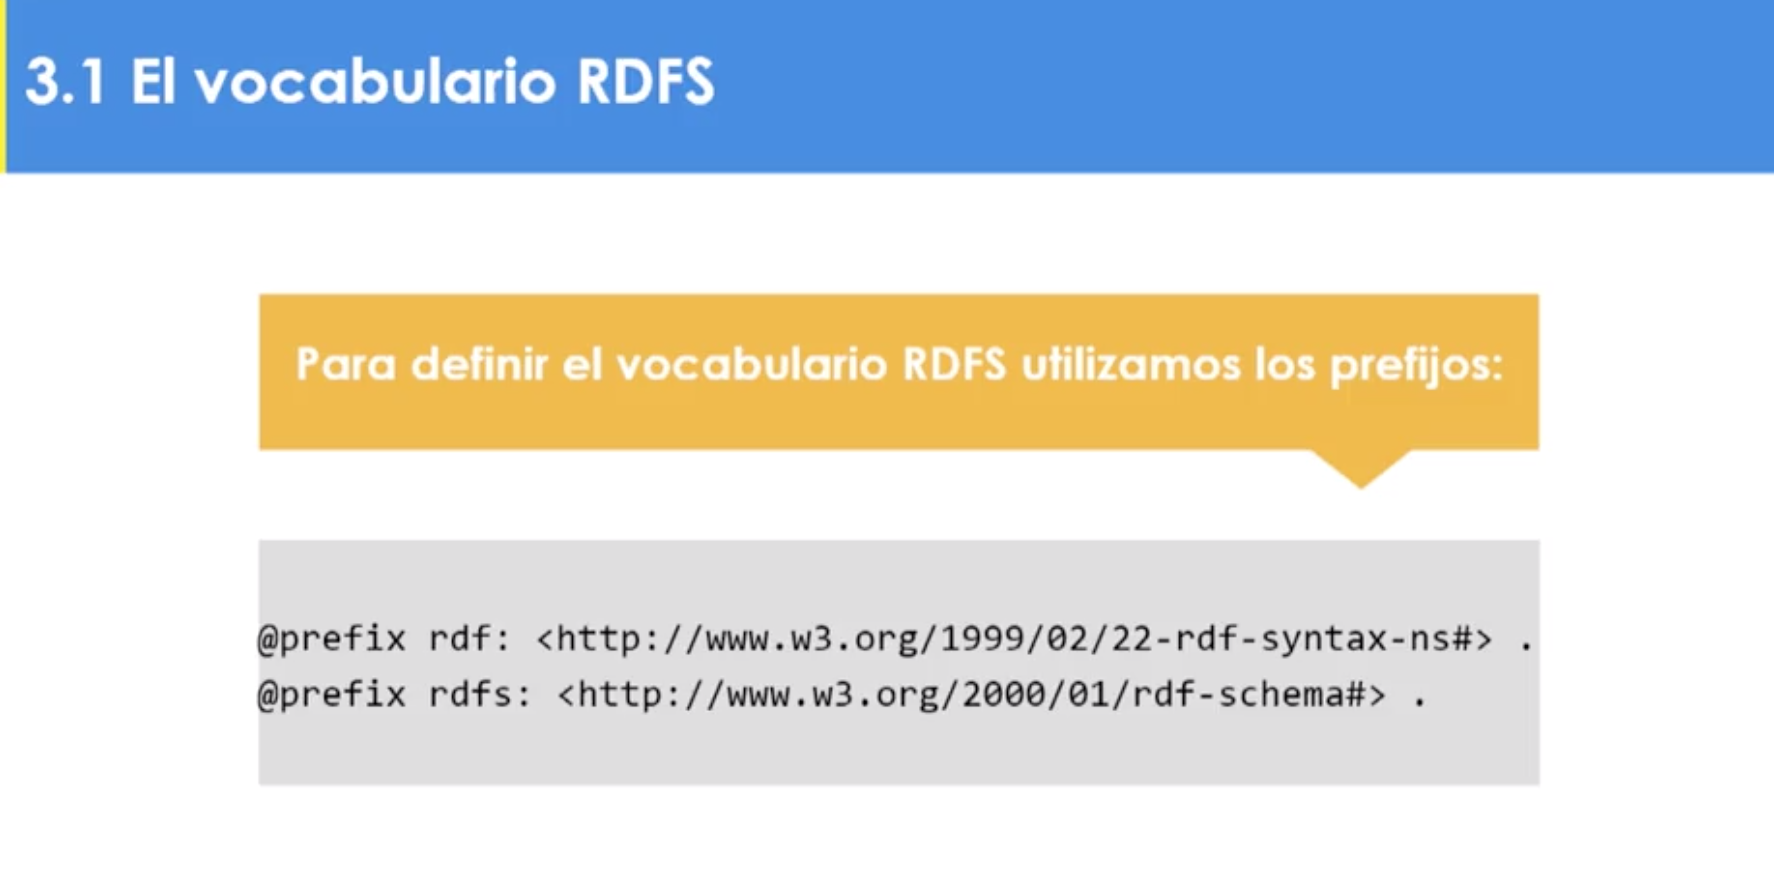
\includegraphics[height=4.5cm]{imagenes/capitulo3/22} 
	\caption{}
	\label{}
\end{figure}

% COURSERA: La Web Semántica: Herramientas para la publicación y extracción efectiva de información en la Web
En primer lugar tenemos las clases y para especificar las clases vamos utilizar el URI rdfs:class recuerde que RDFS en este caso es un prefijo después tenemos las instancias y tipos y para especificarlas vamos a utilizar el URI rdf:type y finalmente tenemos las propiedades y para especificarlas vamos a usar el URI rdf:Property. Entonces comencemos con la noción de clase, recuerde que teníamos tres componentes básicos en RDFS, las clases, las propiedades, las instancias y tipos. Vamos a comenzar por estudiar la noción de clase, una clase es un conjunto de recursos que tienen características comunes y una representación en un mundo real. Por ejemplo la clase jugador de fútbol, cada jugador de fútbol tiene características, o los distintos jugadores de fútbol comparten características comunes, por ejemplo todos ellos tienen que jugar en algún club, tienen que jugar en alguna posición, etcétera.

\begin{figure}[H]
	\centering
	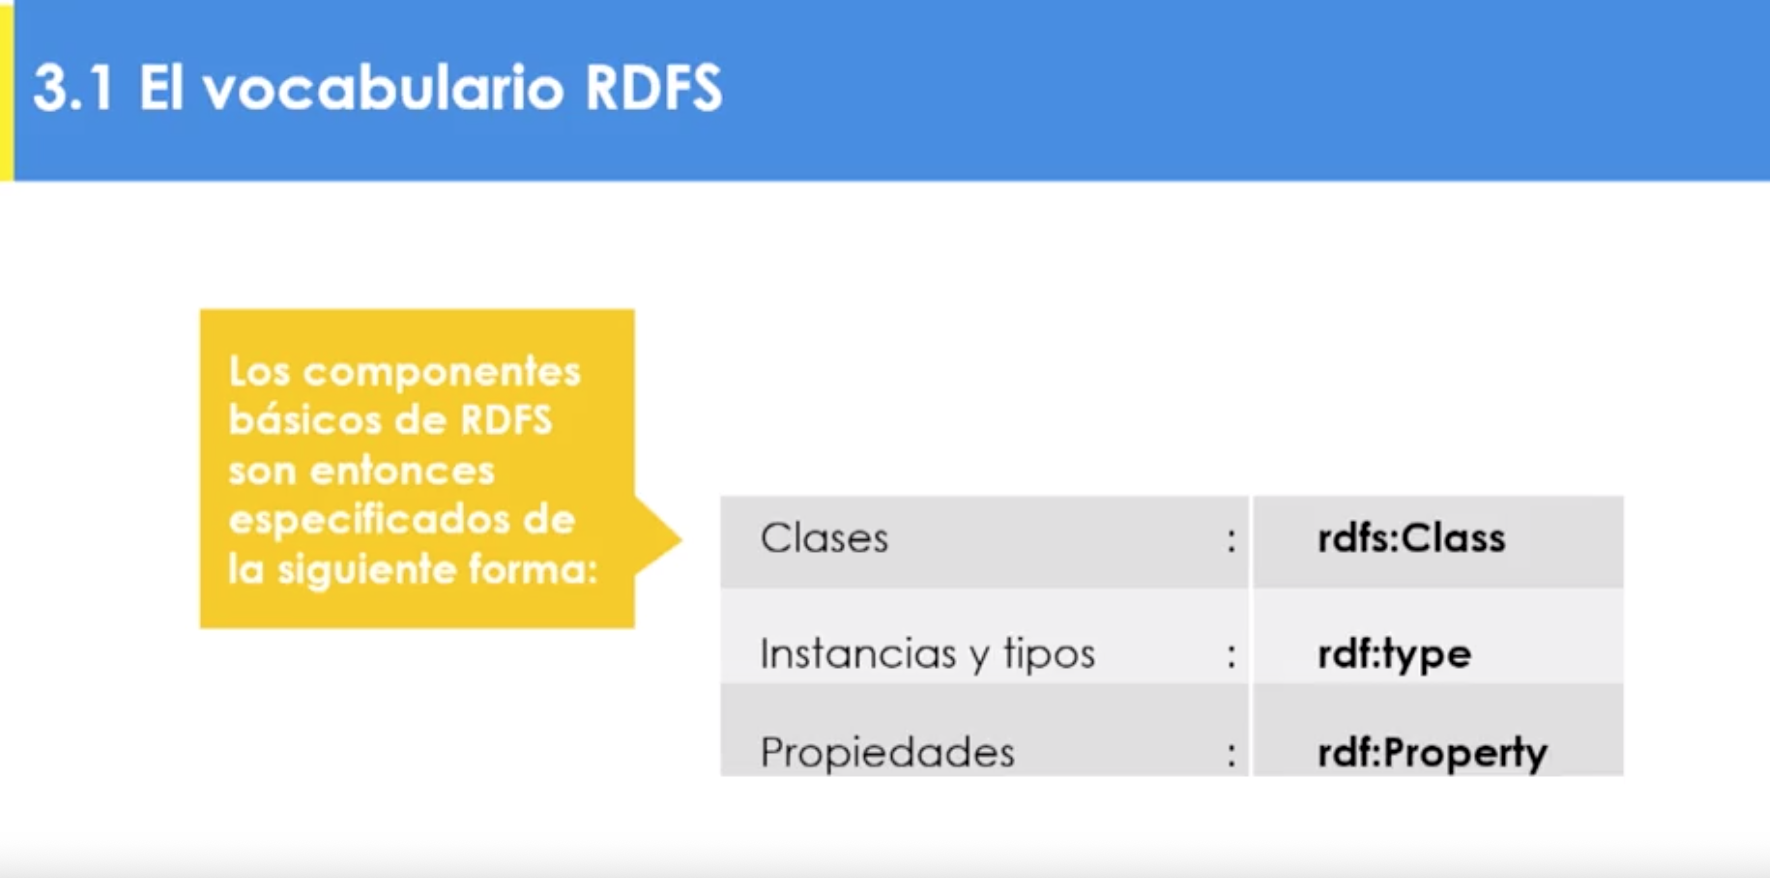
\includegraphics[height=4.5cm]{imagenes/capitulo3/23} 
	\caption{}
	\label{}
\end{figure}

% COURSERA: La Web Semántica: Herramientas para la publicación y extracción efectiva de información en la Web
Otro ejemplo de una clase, por ejemplo podría ser la clase de las personas en este caso tenemos por ejemplo dos jugadores de futbol pero tambien tenemos a Albert Einstein un famoso científico y a Shanti Vasen, también un científico famoso. Cada uno de estos elementos es parte de esta clase persona y la clase persona reúne a un conjunto de elementos que tienen características comunes, por ejemplo todas las personas tienen una edad, tienen una altura, tienen un lugar de nacimiento, etcétera.

% COURSERA: La Web Semántica: Herramientas para la publicación y extracción efectiva de información en la Web
Ahora, ¿cómo se define una clase en RDFS? Para redefinir una clase en RDFS lo que vamos a usar es el vocabulario que estamos describiendo en este video. Primero decimos que vamos a utilizar este prefijo dos puntos que lo que especifica es, www.ejemplo.org y a partir de eso entonces construimos triples que nos indican cuáles son las clases. En este caso tenemos un triple que nos indica que libro es de tipo rdfs:Class, lo que estamos diciendo en este caso entonces que este URI libro lo que representa o lo que es es la clase de los libros.

% COURSERA: La Web Semántica: Herramientas para la publicación y extracción efectiva de información en la Web
Entonces utilizamos nuevamente rdf:type para indicar que el recurso libro es de tipo rdfs:Class, vale decir libro es una clase. Vamos a tener la clase de los libros que reúne un conjunto de elementos que tienen características comunes.

% COURSERA: La Web Semántica: Herramientas para la publicación y extracción efectiva de información en la Web
Ahora sobre la noción de instancia de una clase, un elemento de una clase es llamado una instancia de la clase. Por ejemplo si tenemos la clase de las personas, Albert Einstein es una instancia esto es un elemento de la clase persona.

% COURSERA: La Web Semántica: Herramientas para la publicación y extracción efectiva de información en la Web
Ahora, ¿cómo se definen las clases en RDFS? Para definir las clases, perdón, ¿cómo se definen las instancias en RDFS? Para definir las instancias en RDFS lo que utilizamos es el vocabulario RDFS. En el ejemplo que vamos a ver a continuación decimos que Don Quijote de la Mancha y Cien Años de Soledad son instancias de la clase libro, recuerden que ya definimos la clase libro lo que vamos a hacer ahora es indicar algunas instancias de esta clase. Aquí tenemos el ejemplo completo, nuevamente tenemos un prefijo en el primer triple indicamos que libro es de tipo clase decimos libro rdf:type rdfs:Class. Entonces libro representa una clase y en los dos últimos triples indicamos dos instancias de esta clase decimos :Don_Quijote_de_la_Mancha rdf:type :Libro Es importante recordar aquí que estamos usando URI entonces estamos diciendo el URI que representa a Don Quijote de la Mancha es de tipo el URI que representa el libro, lo que estamos diciendo entonces con este triple es que Don Quijote de la Mancha es de tipo libro, Don Quijote de la Mancha es un libro y en el último triple lo que estamos diciendo es que Cien Años de Soledad es de tipo libro, vale decir Cien Años de Soledad es una instancia de esta clase.

% COURSERA: La Web Semántica: Herramientas para la publicación y extracción efectiva de información en la Web
En resumen lo que hemos visto hoy día es que un modelo de datos permite describir la estructura de los datos y las restricciones que deben cumplir, por ejemplo me gustaría decir que para cada persona debe tener un nombre asociado.

% COURSERA: La Web Semántica: Herramientas para la publicación y extracción efectiva de información en la Web
RDFS Schema, RDF Schema o RDFS es un vocabulario RDF que nos permite definir modelos de datos. El objetivo de RDFS es proveer de los elementos básicos y comunes para la descripción de datos de diversos dominios. Si uno mira diversos dominios se da cuenta que hay ciertos elementos comunes que queremos especificar lo que hace RDF Schema es abstraer estos elementos y los componentes básicos de RDFS son las clases, las instancias y tipos y las propiedades. 

\subsubsection{Propiedades y RDF Schema}

% COURSERA: La Web Semántica: Herramientas para la publicación y extracción efectiva de información en la Web
Hasta ahora, hemos visto los conceptos básicos de RDFS, como son clases e instancias. Ahora vamos a seguir con estos conceptos explicando qué son las propiedades.

% COURSERA: La Web Semántica: Herramientas para la publicación y extracción efectiva de información en la Web
Entonces una propiedad, vamos a, se utiliza para indicar el valor de un atributo de un recurso de datos.

% COURSERA: La Web Semántica: Herramientas para la publicación y extracción efectiva de información en la Web
Como puede ser Messi eh, el nombre de, el primer nombre de Messi es eh, Lionel. O para escribir una relación entre dos recursos de datos, entre los recursos Messi eh, nació en el recurso Rosario.

% COURSERA: La Web Semántica: Herramientas para la publicación y extracción efectiva de información en la Web
Para definir una propiedad en RDFS lo que utilizamos es eh, la, el vocabulario, la palabra eh, Property. Es decir, para definir que firstName, foaf firstName, es una propiedad, decimos foaf firstName es de tipo propiedad. De la misma forma, para definir que birthPlace, el lugar de nacimiento, la propiedad de lugar de nacimiento, es de tipo propiedad, utilizamos dbpprop birthPlace, RDF type, RDF Property. Tal y como estamos mostrando en este, en este ejemplo.

% COURSERA: La Web Semántica: Herramientas para la publicación y extracción efectiva de información en la Web
Además, RDFS nos permite añadir restricciones sobre las propiedades. Consideremos esta relación es, la relación está_casado_con, es obvio que solo las personas pueden casarse. Es decir, una persona está casado con otra persona. No un pájaro está casado con otra persona. Por lo tanto, una restricción obvia es que el sujeto de la relación, de la relación está_casado_con, tiene que ser con una persona. Y de la misma forma, el objeto de la relación estar_casado_con, tiene que ser otra persona.

% COURSERA: La Web Semántica: Herramientas para la publicación y extracción efectiva de información en la Web
Entonces, para definir estas restricciones en nuestros datos, RDFS nos ofrece 2 eh, 2 propiedades, rdfs:domain y rdfs:range. En concreto,en la restricción de dominio o rdfs:domain nos permite especificar cuál debe ser el, o qué tipo debe ser el sujeto de una relación. Es decir, como vemos en el ejemplo, está_casado_con, rdfs:domain persona nos está indicando que la relación estaba, está_casado_con, el sujeto de la relación está_casado_con tiene que ser una persona. Por ejemplo, Pedro está casado con María. Y Pedro es de tipo persona.

% COURSERA: La Web Semántica: Herramientas para la publicación y extracción efectiva de información en la Web
Además, RDFS nos permite definir restricciones sobre los sub, sobre los objetos de, de una relación. De la misma forma que definíamos el dominio, definimos ahora el rango. La re, la re, la restricción de rango nos permite definir una restricción sobre el objeto de la relación. Es decir, definimos como estamos mostrando en el ejemplo la relación está_casado_con rdfs:Range persona nos indica que esta relación tiene que tener como objeto una instancia de la clase persona.

% COURSERA: La Web Semántica: Herramientas para la publicación y extracción efectiva de información en la Web
Un ejemplo más concreto. La relación juega_en, el objeto, el sujeto de la relación tiene que ser una persona. Si tenemos que Messi, que es un, tiene que ser de tipo persona, o más en concreto, jugador de fútbol.

% COURSERA: La Web Semántica: Herramientas para la publicación y extracción efectiva de información en la Web
Además juega_en, el objeto de la relación tiene que ser un club de fútbol.

% COURSERA: La Web Semántica: Herramientas para la publicación y extracción efectiva de información en la Web
Para definir, para definir esto, en RDFS, utilizamos la res, la restricción de dominio rango. Entonces jue, la propiedad juega_en tiene rdfs:domain tiene un dominio, Jugador_de_fútbol, juega_en también tiene un rango, un rdfs:range, Equipo_de_fútbol. Y además, indicamos que juega_en es de tipo propiedad, juega_en, rdf:type, Property. Resumiendo, hemos visto que RDF se puede utilizar para indicar el valor de un atributo de un recurso de datos. También podemos utilizar RDF para definir relaciones entre recursos de datos. Además, RDFS nos permite añadir restricciones sobre el sujeto y el objeto de una relación de datos en RDF.

\subsubsection{Razonamiento en RDF Schema}

% COURSERA: La Web Semántica: Herramientas para la publicación y extracción efectiva de información en la Web
Continuando con nuestro estudio sobre el uso de vocabulario con significado predefinido en RDF hoy vamos a ver algunas técnicas de razonamiento en RDF Schema o RDFS.

% COURSERA: La Web Semántica: Herramientas para la publicación y extracción efectiva de información en la Web
Considere el siguiente grafo RDF que hemos escrito como un archivo, primero tenemos la definición de un prefijo, recuerden que los prefijos nos ayudan a simplificar la notación que utilizamos en los URIs y después tenemos 2 triples. En el primer triple especificamos que jugador de fútbol es de tipo clase, vele decir, decimos que jugador de fútbol es una clase; en el segundo triple, decimos que Carlos es de tipo jugador de fútbol, vale decir, decimos Carlos es un jugador de fútbol.

% COURSERA: La Web Semántica: Herramientas para la publicación y extracción efectiva de información en la Web
Una pregunta, en este caso, es si debería ser Carlos considerado como una persona. Bueno, si pensamos en el dominio de las personas y de los jugadores de fútbol, la respuesta debería ser sí, ya que él es un jugador de fútbol. Pero, no podemos obtener esto desde el grafo RDF, vale decir, no lo podemos obtener de manera automática, el computador no puede inferir en este caso que Carlos es de tipo persona. La pregunta entonces es, ¿cómo podríamos solucionar este problema? Bueno, una alternativa es decir explícitamente que Carlos es de tipo persona, vale decir, incluir en el archivo anterior o en el grafo RDF anterior el siguiente triple, el triple que nos dice Carlos es de tipo persona. Pero hay un problema con esta solución. Bueno, si tenemos un grafo RDF donde guardamos información sobre jugadores de fútbol, por ejemplo, en toda la liga española para decir que cada uno de ellos es una persona, lo que vamos a tener que hacer, vamos a tener que repetir este proceso muchas veces, vale decir, por cada jugador de fútbol vamos a tener que agregar un triple que nos indica que ese jugador de fútbol es de tipo persona. Lo que queremos hacer, por el contrario, o lo que consideramos como una mejor alternativa, es definir una regla general que nos diga que cada jugador de fútbol es de tipo persona, que cada jugador de fútbol es una persona y a partir de esa regla inferir de manera automática que Carlos es de tipo persona.

% COURSERA: La Web Semántica: Herramientas para la publicación y extracción efectiva de información en la Web
Al decir que cada jugador de fútbol es una persona lo que estamos diciendo es que jugador de fútbol es una subclase de la clase persona. Si vemos esto en la transparencia lo vamos a representar como el siguiente ideagrama, lo que estamos diciendo es jugador de fútbol está contenido en persona o cada jugador de fútbol es una persona y llamamos a esto una jerarquía de clases.

% COURSERA: La Web Semántica: Herramientas para la publicación y extracción efectiva de información en la Web
El vocabulario RDFS nos permite especificar jerarquías de clases, recuerde que RDFS es un vocabulario RDF que nos permite decir, especificar ciertas reglas generales, decir cosas sobre el dominio que estamos describiendo, en particular, podemos declarar jerarquías de clase en RDFS y para esto utilizamos el URI rdfs:subclassOf De nuevo, recuerde que, como RDFS es un vocabulario RDF, cada componente de este vocabulario está especificado por un URI y en este caso particular la URI que estamos utilizando tenemos además un prefijo que es el prefijo rdfs.

% COURSERA: La Web Semántica: Herramientas para la publicación y extracción efectiva de información en la Web
Entonces, en nuestro ejemplo anterior, podemos decir que la clase jugador de fútbol es una subclase de la clase persona, utilizando el siguiente triple. Nótese que, en la primera línea, estamos diciendo cuál es el prefijo que estamos utilizando, que es rdfs, ése es el prefijo, y en la tercera línea de este archivo lo que estamos diciendo es jugador de fútbol es una subclase de persona. Eso lo decimos con jugador de fútbol rdfs subclassOf persona.

% COURSERA: La Web Semántica: Herramientas para la publicación y extracción efectiva de información en la Web
Ahora lo que queremos hacer a partir de estos triples es razonar de manera automática. Volvamos al ejemplo anterior. En este caso, tenemos 2 triples, uno que nos dice que Carlos es de tipo jugador de fútbol y además tenemos un triple que nos dice que jugador de fútbol es una subclase de persona. Lo que queremos hacer en este caso es obtener de manera automática que Carlos es de tipo persona, vale decir, nos gustaría inferir, nos gustaría que una aplicación computacional pudiera inferir que Carlos es de tipo persona a partir de estos dos triples. El mecanismo de razonamiento RDFS nos permite inferir nuevos triples a partir de los existentes como mostrábamos en el ejemplo anterior. Tenemos un conjunto de triples utilizamos el significado de este vocabulario e inferimos nuevos triples y estos triples son considerados como parte del grafo RDF, vale decir, si es que nosotros nos preguntamos en el ejemplo anterior si es que Carlos era de tipo persona, la respuesta que vamos a obtener es sí, ya que este triple se puede inferir de manera automática a partir de los otros triples. Ahora, este mecanismo, el mecanismo de razonamiento de RDFS lo que utiliza es el significado de las distintas, de los distintos componentes del vocabulario RDFS que hemos visto en este video y en los videos anteriores. Por ejemplo, rdfs class, decimos que algo es una clase, rdfs:type rdf:property, rdfs:domain, rdf:range y rdf:subclassOf. Ahora, este mecanismo de inferencia de RDFS se traduce en una serie de reglas de inferencia. Ahora, ¿cómo se ven estas reglas de inferencia? Siempre se ven de la misma forma, se ven, dicen algo como a partir de este conjunto de triples infiera el siguiente triple, y estas declaraciones son generales. Por ejemplo, la manera que representamos el razonamiento que hicimos en las transparencias anteriores lo que decimos es lo siguiente: a partir de los triples A es de tipo C y C es subclase de D infiera el triple A es de tipo D. Nuevamente es importante recalcar acá, que lo que estamos diciendo es si sabemos que A es de tipo C y sabemos que C es una subclase de D, entonces, podemos inferir, y vamos a hacer esto de manera automática, que A es de tipo D. Gráficamente esto se puede mostrar de la siguiente forma, lo que estamos diciendo es C es una clase y está contenido en la clase D. Entonces si A era un elemento de C o A era de tipo C, podemos inferir que A también era de tipo D, o sea, que A está contenido en D. El mecanismo de inferencia de RDFS incluye otras reglas como esta. Como resumen, lo que hemos visto en este video es que RDFS tiene un componente que permite indicar que una clase es una subclase de otra y esto es lo que llamamos una jerarquía de clases. Por ejemplo, podemos decir que jugador de fútbol es una subclase de persona. RDFS tiene un mecanismo de razonamiento que permite inferir nuevos triples a partir de los existentes. Tenemos un conjunto de triples utilizamos el significado ya estandarizado de los componentes de RDFS e inferimos nuevos triples. Y este mecanismo, bueno, utiliza el significado del vocabulario RDFS y se traduce en una serie de reglas de inferencias para RDFS. Por ejemplo, una regla de inferencia que nos dice que si sabemos que A era de tipo C y C subclase de D, entonces podemos inferir que A es de tipo D.


\subsubsection{Reglas de Inferencia en RDF Schema}

% COURSERA: La Web Semántica: Herramientas para la publicación y extracción efectiva de información en la Web
Continuando con nuestro estudio sobre el uso de vocabularios con significado predefinido en RDF. Hoy vamos a ver algunas reglas de inferencia en RDF Schema o RDFS.

% COURSERA: La Web Semántica: Herramientas para la publicación y extracción efectiva de información en la Web
Al igual que cuando hablamos de clase, las propiedades también pueden tener jerarquía. Por ejemplo, considere la siguiente figura. En esta figura podemos ver una propiedad es hermano de, que nos ayuda a especificar que cierta persona es hermano de otra persona, y también tenemos la propiedad es pariente de, y también nos permite especificar que una persona es pariente de otra persona. En este caso tenemos una jerarquía de propiedades, porque esperamos que si A es hermano de B, entonces A es pariente de B. En ese sentido, es pariente de, es más general.

% COURSERA: La Web Semántica: Herramientas para la publicación y extracción efectiva de información en la Web
RDFS tiene un componente que nos permite indicar que una cierta propiedad es una subpropiedad de otra. Recuerde que RDFS es un vocabulario de RDF, que nos permite especificar reglas que tiene que satisfacer un cierto dominio. Y como es un vocabulario RDF cada uno de sus componentes es especificado por un URI. En este caso para especificar su propiedad, utilizamos el URI RDFS: subPropertyOf. Recuerden también que en este caso estamos usando un prefijo para simplificar la notación del URI, y este prefijo está representado por RDFS.

% COURSERA: La Web Semántica: Herramientas para la publicación y extracción efectiva de información en la Web
Entonces, podemos decir en RDFS que la propiedad es hermano de, es una subpropiedad de la propiedad es pariente de, y para eso utilizamos el triple que hemos mostrado en la transparencia. Nótese que en este archivo primero estamos declarando el prefijo RDFS que vamos a estar utilizando en este video, y en el último triple de este archivo estamos declarando que es hermano de es subpropiedad de es pariente de, lo cual hacemos a través del triple que nos indica es hermano de, RDFS:subPropertyOf es pariente de. ¿Qué queremos hacer con estos triples? Bueno, queremos hacer razonamiento. O sea, a partir de los dos triples, de los dos triples que podemos ver a continuación, un triple que nos dice que Joaquín Phoenix es hermano de River Phoenix, y que es hermano de es una subpropiedad de es pariente de. Nos gustaría deducir de manera automática que Joaquín Phoenix es pariente de River Phoenix. Y esto es lo que podemos lograr a través de RDFS, el computador o las aplicaciones computacionales van a poder inferir de manera automática que Joaquín Phoenix es pariente de River Phoenix a partir de los dos triples que teníamos arriba. ¿Sí? Como habíamos visto en el video anterior, estas formas de razonamiento de RDFS se traducen en reglas de inferencia, en el caso particular del ejemplo que vimos en este video, la regla de inferencia se debe a la siguiente forma. Dice, a partir de los triples A, P, B, y P es una subpropiedad de Q, infiere al triple A, Q, B. Lo que estamos diciendo en este caso es, si el sujeto A está relacionado con el objeto B a través de la propiedad P, y sabemos que P es una subpropiedad de la propiedad Q, entonces podemos inferir que el sujeto A está relacionado con el objeto B a través de la propiedad Q. RDFS tiene otras reglas de inferencia que nos permiten deducir triples a partir de triples existentes. Las otras reglas de inferencia fundamentales en RDF son utilizadas para inferir nuevas relaciones de subclase utilizando jerarquías de clases. Inferir nuevas relaciones de propiedad utilizando jerarquías de propiedades. E inferir a qué clase pertenece un objeto utilizando el dominio o el rango de una propiedad. A continuación, vamos a ver estas distintas reglas. En primer lugar, veamos la regla de inferencia sobre jerarquías de clases. En este ejemplo tenemos tres clases, tenemos la clase de los jugadores de fútbol, la clase de los deportistas y la clase de las personas. Y lo que sabemos es que, si cada jugador de fútbol es un deportista y cada deportista es una persona. Lo que nos gustaría inferir entonces, es que cada jugador de fútbol es una persona. Gráficamente podemos representar esto de la siguiente forma, tenemos la clase de los jugadores de fútbol, que está contenida en la clase de los deportistas, y que a su vez la clase de los deportistas está contenido en la clase de las personas. Entonces, lo que nos gustaría deducir es que la clase de los jugadores de fútbol está contenido en la clase de las personas. Como mencionábamos anteriormente, esta forma de razonamiento RDFS se traduce en una regla de inferencia. En este caso la regla de inferencia se ve de la siguiente forma. Decimos si tenemos los triples A es subclase de B, y B es subclase de C, entonces se puede inferir el triple A es subclase de C. Recuerde que inferir significa que consideramos el triple A es subclase de C como parte de nuestro grafo RDF, y que una aplicación computacional va a deducir este triple de manera automática. Al igual que para las jerarquías de clases, tenemos una regla para las jerarquías de propiedades, que es muy similar, y que se ve de la siguiente forma. Dice a partir de los triples P es subpropiedad de Q, y Q es subpropiedad de R, infiere al triple P es subpropiedad de R. Lo que estamos diciendo en este caso entonces es que, si sabemos que la propiedad P es una subpropiedad de la propiedad Q, y sabemos que la propiedad Q es una subpropiedad de la propiedad R, entonces podemos deducir, y vamos a hacer esto de manera automática, que P es una subpropiedad de R.

% COURSERA: La Web Semántica: Herramientas para la publicación y extracción efectiva de información en la Web
En tercer lugar tenemos una regla de inferencia para el dominio de una propiedad. Veamos un ejemplo sobre esto. En este caso tenemos la propiedad juega en, y tenemos que Messi juega en Barcelona. ¿Qué sabemos sobre esta propiedad? Sabemos que el dominio de esta propiedad es la clase jugador de fútbol. Lo que nos gustaría deducir entonces, es que Lionel Messi es un jugador de fútbol. Vale decir lo que queremos hacer formalmente es deducir un triple de la forma dbpedia:Lionel Messi es de tipo jugador de fútbol. ¿Cómo hacemos esto? Bueno, para hacer esto tenemos la siguiente regla de inferencia. Y esta regla de inferencia es la regla de inferencia que está relacionada con el dominio de una propiedad. Lo que tenemos en este caso es lo siguiente, si tenemos el triple A, P, B, y tenemos el triple P dominio C, entonces inferimos el triple A tipo C. Lo que estamos diciendo en otras palabras, es que si sabemos que el sujeto A está relacionado con el objeto B a través de la propiedad P, y sabemos que el dominio de P es la clase C, vale decir todos los sujetos que tenemos en esta relación tienen que ser de tipo C, bueno, lo que vamos a inferir entonces es que A es de tipo C.

% COURSERA: La Web Semántica: Herramientas para la publicación y extracción efectiva de información en la Web
Bueno, esta forma de razonamiento se traduce en la siguiente regla de inferencia para el domino de una propiedad. Esta regla de inferencia nos dice, si tenemos el triple A P B, y tenemos que el triple P dominio C, entonces podemos inferir el triple A tipo C. Lo que estamos diciendo en este caso es, si el sujeto A está relacionado con el objeto B a través de la propiedad P y sabemos que el dominio de P es C, vale decir sabemos que todos los sujetos que estén relacionados a través de la propiedad P tienen que ser de tipo C, entonces lo que vamos a inferir es que A es de tipo C en este caso. Al igual que para el caso del dominio, tenemos una regla de inferencia para el rango de una propiedad que es muy similar. En este caso lo que decimos es lo siguiente, si sabemos que tenemos el triple A P B, y sabemos que el rango de P es D, entonces podemos deducir que B es de tipo D. En otras palabras, si tenemos que el sujeto A está relacionado con el objeto B a través de la propiedad P, y sabemos que el rango de la propiedad es B, entonces sabemos que los objetos que están relacionados a través de esta propiedad P, tienen que ser de tipo D. Entonces podemos inferir en este caso que B es de tipo D.

% COURSERA: La Web Semántica: Herramientas para la publicación y extracción efectiva de información en la Web
En resumen, hemos visto en este video que RDFS tiene un componente que permite indicar que una propiedad es una subpropiedad de otra. Por ejemplo podemos indicar que es hermano de es una subpropiedad de es pariente de. RDFS tiene reglas de inferencia sobre jerarquías de clases y propiedades que nos permiten inferir nuevas jerarquías de clases a partir de las dadas y nuevas jerarquías de propiedades a partir de las dadas, y RDFS además tiene reglas de inferencia para el dominio y rango de una propiedad.

\subsection{OWL}

% COURSERA: La Web Semántica: Herramientas para la publicación y extracción efectiva de información en la Web
Hola, bienvenidos nuestro curso de la Web Semántica. En este video veremos los primeros componentes del Web Ontology Language o OWL. OWL es un vocabulario RDF, donde cada palabra tiene un significado bien definido y estandarizado. Recuerde que hasta ahora hemos visto varios vocabularios RDF, en particular RDFS o RDF Schema.

% COURSERA: La Web Semántica: Herramientas para la publicación y extracción efectiva de información en la Web
El objetivo de OWL es proveer elementos avanzados para la descripción de diversos dominios, además de proveer de un sistema de razonamiento para estos datos.

% COURSERA: La Web Semántica: Herramientas para la publicación y extracción efectiva de información en la Web
El objetivo de OWL es similar al objetivo que teníamos detrás de RDF Schema o RDFS, pero lo que nos provee OWL es un vocabulario que nos permite construir reglas más avanzadas cuando estamos describiendo un dominio.

% COURSERA: La Web Semántica: Herramientas para la publicación y extracción efectiva de información en la Web
Es importante en este punto recordar los componentes de RDFS. En primer lugar teníamos las clases que agrupan a objetos o a recursos que tienen características comunes. Por ejemplo la clase de las personas, la clase de los jugadores de fútbol, tenemos instancias y tipos que nos permitían decir que ciertos recursos pertenecían a una clase. Por ejemplo, Leonel Messi es de tipo jugador de fútbol. Va a decir Leonel Messi es un jugador de futbol y finalmente teníamos las propiedades o relaciones que nos permitían establecer relaciones en los recursos. Por ejemplo, podíamos decir que Leonel Messi juega en el recurso Barcelona, o en el equipo de fútbol Barcelona.

% COURSERA: La Web Semántica: Herramientas para la publicación y extracción efectiva de información en la Web
OWL extiende a RDFS, en esta figura usted ver los cuatro componentes esenciales de OWL. Tres de estos componentes son idénticos a los de RDFS. Tenemos clases, tenemos propiedades, y tenemos instancias y tipos. En el caso de OWL también hablamos de individuos como un sinónimo de instancia.

% COURSERA: La Web Semántica: Herramientas para la publicación y extracción efectiva de información en la Web
Y en el caso de OWL, agregamos adicionalmente mecanismos que nos permiten definir axiomas o restricciones.

% COURSERA: La Web Semántica: Herramientas para la publicación y extracción efectiva de información en la Web
Entonces los componentes básicos de OWL son especificados de la siguiente forma: Para hablar de que algo es una clase, usamos el URI owl:Class, para hablar de instancias y tipos, hablamos de, rdf:type, esto al igual que en RDFS.

% COURSERA: La Web Semántica: Herramientas para la publicación y extracción efectiva de información en la Web
Para hablar de propiedades entre valores de datos, por ejemplo, para indicar que la edad de Messi es un cierto número, usamos, owl:DatatypeProperty. Para hablar de propiedades entre clases, hablamos de owl:ObjectProperty, y para definir axiomas o restricciones sobre clases y propiedades, utilizamos algunos predicados especiales que vamos a ver en los siguientes videos. Entonces veamos un primer ejemplo en OWL. En este caso vamos a definir una clase. Al igual como lo hacíamos en RDFS, primero definimos un cierto prefijo. En este prefijo es el prefijo, example.org, y en este caso decimos que libro es de tipo clase, para decir esto usamos el triple libro rdf:type, owl:Class, en este caso estamos usando rdf.type para indicar que el recurso libro es de tipo owl:Class, vale decir: libro es una clase.

% COURSERA: La Web Semántica: Herramientas para la publicación y extracción efectiva de información en la Web
El recurso libro en este caso también es conocido como una instancia o individuo en OWL. Veamos un segundo ejemplo más avanzado. El objetivo de este ejemplo es demostrar algunas de las funcionalidades nuevas que tiene OWL y que no estaban en RDFS. Entonces considere el siguiente grafo RDF. Nuevamente tenemos un prefijo que es, example.org y estamos indicando en este caso que el libro es una clase. En el primer triple, libro rdf:type owl:Class, En el segundo triple estamos especificando que el libro de aventuras también es de tipo clase, Y el en el tercer triple indicamos que el libro de historia también es de tipo clase. En este caso, nos gustaría decir que la clase libro es la unión de la clase libro de aventuras y libro de historia. Vale decir, cada libro de aventuras es un libro, cada libro de historia es un libro, pero adicional adicionalmente, cada libro, sabemos que tiene que ser o un libro de aventuras o un libro de historias. Una pregunta obvia en este punto es, ¿Si podemos especificar esto en un RDFS? y la respuesta es no.

% COURSERA: La Web Semántica: Herramientas para la publicación y extracción efectiva de información en la Web
En RDFS no podemos decir que la clase libro es la unión de la clase libro de aventura ni libro de historia, vale decir, el vocabulario no nos provee de ningún componente que nos permita especificar que una clase se construye como la unión de otras dos clases. En cambio, en OWL sí podemos decir esto, y para esto vamos a utilizar el componente del vocabulario owl:unionOF. Y esto nos va a permitir decir de manera precisa que el libro es la unión de las clases libro de aventura y libro de historia.

% COURSERA: La Web Semántica: Herramientas para la publicación y extracción efectiva de información en la Web
Como resumen, OWL es un vocabulario que ofrece una gran expresividad para crear un modelo de datos. Los componentes principales de OWL son las clases, las propiedades sobre clases y sobre valores de datos, las instancias o individuos, y las restricciones o axiomas. Y los axiomas o restricciones de OWL se especifican mediante un vocabulario particular y se aplican a propiedades y a clases.

\subsection{Propiedades OWL}

% COURSERA: La Web Semántica: Herramientas para la publicación y extracción efectiva de información en la Web
En este video lo que vamos a ver son propiedades en OWL. Vamos a ver propiedades y también algunas restricciones que podemos aplicar a estas propiedades.

% COURSERA: La Web Semántica: Herramientas para la publicación y extracción efectiva de información en la Web
Pero, ¿qué son las propiedades? Las propiedades en OWL son, indican relaciones entre clases o entre individuales. Las relaciones object properties son las que describen relaciones entre clases. Por ejemplo, la relación vive en es de tipo object owL:ObjectProperty y lo que indica es que las instancias o los individuales de una determinada clase viven en los individuales de otra determinada clase. Mientras tanto, las relaciones que son del tipo data type properties, lo que hacen es describir las relaciones entre individuos y literales. Por ejemplo edad, la propiedad edad, es de tipo owl:DataTypeProperty. Edad, se aplica a personas y el objeto de esta relación es, un literal habitualmente. Bien, ¿cómo podemos definir estas propiedades? Bien, utilizamos como ven en este ejemplo, definimos primero los prefijos y después indicamos qué arrienda es de tipo object property mediante el triple arrienda rdf:type owl:ObjectProperty. De la misma forma indicamos que edad es del tipo data property con el triple edad rdf:type owl:DataTypeProperty. Utilizamos el rdf type para indicar que arrienda es del tipo owl property y edad es del tipo owl object property.

% COURSERA: La Web Semántica: Herramientas para la publicación y extracción efectiva de información en la Web
Bien, una vez definimos unas propiedades también podemos restringir estas propiedades. En este ejemplo podemos restringir la propiedad arrienda, indicando que solo las personas pueden arrendar, es decir, el sujeto en esta relación, tiene que ser de tipo persona. ¿Cómo podemos hacer esto en OWL? Pues lo que hacemos es reutilizar el vocabulario que nos daba RDFS en nuestros triples.

% COURSERA: La Web Semántica: Herramientas para la publicación y extracción efectiva de información en la Web
Por ejemplo, para restringir el dominio de una relación, es decir, el sujeto de la relación, utilizamos rdf domain y para restringir el objeto de la relación, utilizamos rdfs domain.

% COURSERA: La Web Semántica: Herramientas para la publicación y extracción efectiva de información en la Web
Bien, una restricción de dominio permite clasificar los sujetos de una relación. Aquí vemos el triple, los triples. Primero definimos los prefijos y después definimos que arrienda es del tipo owl:ObjectProperty y arrienda es de rdfs:domain. Persona, es decir, el sujeto de la relación tiene que ser de tipo persona.

% COURSERA: La Web Semántica: Herramientas para la publicación y extracción efectiva de información en la Web
En este ejemplo, Carlos es del tipo persona y solo las personas pueden arrendar. Entonces Carlos, el sujeto, debe ser de tipo persona. Ahora vamos a restringir el rango, es decir, el objeto de la relación. Primero utilizamos como ven en el ejemplo, los prefijos habituales, y definimos que arrienda es del tipo rdf:type, object property y que arrienda rdfs:range casa, es decir, el rango de la propiedad, el objeto de la propiedad tiene que ser de tipo casa.

% COURSERA: La Web Semántica: Herramientas para la publicación y extracción efectiva de información en la Web
Y aquí vemos el ejemplo anterior. Vemos que casa 1 tiene que ser de tipo casa para que la propiedad, la restricción sobre la propiedad sea verdadera.

% COURSERA: La Web Semántica: Herramientas para la publicación y extracción efectiva de información en la Web
Ahora vamos a pasar a ver un ejemplo con data type properties. En este ejemplo lo que hacemos es definir la propiedad edad que es del tipo data type property. Como ven en el ejemplo, después de los prefijos habituales edad rdf:type owl:DataTypeProperty. Hacemos que arrienda rdfs:domain persona y que edad rdfs:range non negative integer. Es decir, edad, el rango de la propiedad edad, el objeto de la relación tiene que ser un entero positivo. Uno no puede tener menos cinco años, pues. Ya, una vez hemos definido las, los data type property y los object property vamos a ver, qué restricciones adicionales, además del rango y dominio, podemos utilizar, podemos utilizar con OWL. Una propiedad bastante conocida es la propiedad transitiva. OWL nos permite especificar restricción de transitividad a nuestras propiedades. Por ejemplo, si A esta relacionado con B y B está relacionado con A, a través de la misma relación esta relación es transitiva. Entonces se cumple que A está relacionado con C. Un ejemplo es la propiedad es menor que rdf:type owl:TransitiveProperty. Similarmente, en forma similar, tenemos las propiedades simétricas. Si A está relacionado con B, y la relación es simétrica, entonces B está relacionado con A. Un ejemplo es la relación vive con. Vive con, si alguien vive con alguien, pues, la otra persona también. Y se define como vive con rdf:type owl:SymmetricProperty, tal y como ven en la transparencia.

% COURSERA: La Web Semántica: Herramientas para la publicación y extracción efectiva de información en la Web
Vamos a ver ejemplos concretos. Por ejemplo, Carlos es menor que Felipe y Felipe es menor que María. Si es la relación es menor que, definida como una relación transitiva, entonces se infiere el sistema, infiere que Carlos es menor que María. Ahora una propiedad simétrica. Carlos vive con Felipe. Si hemos definido que vive con es una propiedad simétrica, entonces, el sistema infiere automáticamente que Felipe vive con Carlos.

% COURSERA: La Web Semántica: Herramientas para la publicación y extracción efectiva de información en la Web
En resumen, las propiedades en OWL son de dos tipos. Property para definir las relaciones entre clases y data type property para describir valores de instancia o individuos.

% COURSERA: La Web Semántica: Herramientas para la publicación y extracción efectiva de información en la Web
Además es posible definir restricciones de rango y dominio sobre estas propiedades, utilizando el vocabulario RDFS.

% COURSERA: La Web Semántica: Herramientas para la publicación y extracción efectiva de información en la Web
Finalmente en el OWL, es posible declarar propiedades que satisfacen condiciones adicionales, como transitividad o simetría.

% ONTOLOGÍA - \section{Ontologías}

% Libro Geospatial Semantic Web
El término “Ontología” viene de la Filosofía: El estudio de la naturaleza de la existencia. Tiene un significado distinto en Informática: "Una ontología es una especificación formal y explícita de una conceptualización". 

% Libro Geospatial Semantic Web
Proporcionan un entendimiento compartido de un dominio: interoperabilidad semántica.
– Solucionan diferencias en terminología.
– Hay que establecer correspondencias entre ontologías.
Útiles para organizar y navegar sitios Web.

% Hay tres tipo de ontologías
% Deberíamos ver como dar la definición de la ontología básica, y luego ver dicha definición para la Web Semántica
% Poner ejemplos de ontologías
% Existen ontologías geoespaciales y ontologías básicas, estaría bien centrarse en ambas
% Ver los estándares
%  Ejemplo

Hay varios lenguajes de ontología disponibles para codificar la ontología.

% Hay tres tipo de ontologías
% Deberíamos ver como dar la definición de la ontología básica, y luego ver dicha definición para la Web Semántica
% Poner ejemplos de ontologías
% Existen ontologías geoespaciales y ontologías básicas, estaría bien centrarse en ambas

% Ver los estándares

% Ontologías y razonamiento automatizado

% http://www.fgcsic.es/lychnos/es_es/articulos/construyendo_una_web_semantica
En último término, la visión de una web semántica, tal y como la plantearon Berners-Lee y sus colaboradores hace diez años, incluye también la posibilidad de razonar y sacar conclusiones lógicas de forma automatizada a partir de los datos publicados en la Web. Así pues, del hecho de que España comparta frontera con Francia y de que compartir frontera signifique que las regiones geográficas que constituyen estos países son contiguas, se debería poder deducir automáticamente que uno puede desplazarse de España a Francia por tierra sin tener que cruzar un tercer país. Esto, requiere que dispongamos de definiciones formales —es decir procesables por una computadora— de lo que significa la relación de contigüidad entre regiones espaciales y su relación con el desplazamiento continuo en regiones del espacio.

% http://www.fgcsic.es/lychnos/es_es/articulos/construyendo_una_web_semantica
Esta información adicional que complementa los datos y con la cual se pueden deducir relaciones semánticas sin que estén explícitamente representadas en el conjunto de datos es lo que se llama una ontología. Habitualmente se trata de un conjunto de expresiones en un lenguaje formal basado en la lógica que describe con mayor o menor detalle los conceptos y sus interrelaciones de un área de conocimiento en particular (por ejemplo de la geografía en general o de la de España en particular). Para poder publicar y razonar con ontologías en la Web se recomienda utilizar el Web Ontology Language (OWL).

% https://www.researchgate.net/publication/216537707_La_Web_semantica_y_las_tecnologias_del_lenguaje_humano
Como ya se ha visto en el esquema de Berners-Lee, las ontologías son una de las piezas clave de la web semántica. Se trata de especificaciones formales y explícitas que representan los conceptos de un determinado dominio y sus relaciones (Gruber, 93). Es decir, son un modelo abstracto de un dominio, donde los conceptos utilizados están claramente definidos y pueden ser utilizados directamente por los agentes. De este modo los agentes pueden interpretar el significado de un texto y a partir de aquí buscar e integrar datos.

% https://www.researchgate.net/publication/216537707_La_Web_semantica_y_las_tecnologias_del_lenguaje_humano
Las ontologías se usan principalmente para favorecer la comunicación entre organizaciones, personas y aplicaciones, permitiendo la interoperabilidad entre sistemas informáticos con el objetivo final de llegar al razonamiento automático. Gracias al conocimiento almacenado en las ontologías, los agentes podrán extraer automáticamente datos de las páginas web, procesarlos y sacar conclusiones de ellos; sin embargo, esta funcionalidad actualmente todavía está lejos de ser una realidad.

% https://www.researchgate.net/publication/216537707_La_Web_semantica_y_las_tecnologias_del_lenguaje_humano
La formalización del conocimiento en las ontologías es una de las barreras iniciales para la implantación de la web semántica, ya que la construcción de ontologías es un proceso extremadamente lento, costoso y propenso a los errores, y además requiere un gran esfuerzo y especialización que muchas organizaciones no tienen a su alcance. Por tanto, es necesario crear mecanismos para promover su desarrollo de una forma (semi)automática.

% 6.3.2.1 El aprendizaje de ontologías

% https://www.researchgate.net/publication/216537707_La_Web_semantica_y_las_tecnologias_del_lenguaje_humano
El aprendizaje de ontologías se define como la adquisición de los términos que representan un dominio a partir de datos. Tiene por objetivo principal crear una jerarquía de conceptos, es decir, una taxonomía. Existen diferentes modalidades de sistemas de aprendizaje de ontologías dependiendo de los tipos de datos de entrada utilizados para el aprendizaje: textos, diccionarios, bases de conocimiento, datos semi- estructurados y bases de datos (Maedche, 01).

% 6.2.3.2 La población de ontologías

% https://www.researchgate.net/publication/216537707_La_Web_semantica_y_las_tecnologias_del_lenguaje_humano
La población de ontologías consiste en enriquecer una ontología con las instancias de los conceptos y de las relaciones extraídas de los textos de una forma (semi)automática. Muchas de las aproximaciones realizadas a partir de este enfoque se basan en la extracción de las entidades. Es un proceso muy semejante al descrito en la figura 4, aunque no tan complejo. Concretamente se centran en la identificación, extracción y clasificación de las entidades nombradas (EN); es decir, de los nombres de personas y de organizaciones, y también de los lugares, fechas y medidas (porcentajes, peso, monedas, tiempo) pues se considera que en ellas reside gran parte del contenido semántico de un texto.

% https://www.researchgate.net/publication/216537707_La_Web_semantica_y_las_tecnologias_del_lenguaje_humano
El proceso consiste en reconocer las EN como instancias de alguno de los conceptos de la ontología y de este modo ir poblando una ontología. El reconocimiento de EN no es un proceso trivial ya que existen algunos conflictos que requieren la aplicación de técnicas lingüísticas para resolverlos como veremos en los siguientes ejemplos.

% https://www.researchgate.net/publication/216537707_La_Web_semantica_y_las_tecnologias_del_lenguaje_humano
En un texto pueden existir distintas variantes de una misma instancia; por ejemplo, Juan López, Sr. López, Juan, él, son distintas formas utilizadas para referirse a la misma persona. Tienen que aplicarse técnicas de correferencia y de resolución de la anáfora pronominal para identificar que expresiones utilizadas anteriormente en el texto inciden directamente en la interpretación de los elementos que aparecen más tarde. Por otro lado, una EN puede ser ambigua, tener dos o más posibles interpretaciones, por ejemplo el término Adolfo Domínguez puede referirse tanto a una persona como a una organización, por tanto, para seleccionar el valor adecuado deben aplicarse técnicas de desambiguación.

\subsection{SPARQL}

% COURSERA: La Web Semántica: Herramientas para la publicación y extracción efectiva de información en la Web
Hola, bienvenido a nuestro curso sobre la web semántica, en este video comenzaremos a ver algunas de la nociones básicas sobre el lenguaje de consulta SPARQL, en particular veremos la nociones de variables y patrones en SPARQL. Como ya hemos mencionado en los videos anteriores en la web existe una multitud de base de datos de RDF, por ejemplo dbpedia, que es la representación en RDF en wikipedia la dbpedia en español y IMDB que es una base de películas, etcétera. Muchas de estas bases RDF permiten acceder a sus datos utilizando el lenguaje de consulta SPARQL, recuerde que SPARQL es un lenguaje que nos permite escribir de manera precisa la información que queremos extraer y que es procesable por un computador, vale decir un computador puede de manera automática construir las respuestas de una consulta SPARQL. Entonces en esta base de datos RDF nos permiten utilizar este lenguaje SPARQL y la forma de hacerlo es a través de lo que es llamado un SPARQL endpoint, que es un servicio web donde uno puede colocar este tipos de consultas. En esta transparencia puede ver la dirección de dos de estos servicios web, la primera de ellas es el SPARQL endpoint de dbpedia que es dbpedia.org/sparql, la segunda es el SPARQL endpoint de dbpedia en español.

% COURSERA: La Web Semántica: Herramientas para la publicación y extracción efectiva de información en la Web
En el caso de dbpedia es posible acceder a los datos utilizando en primer lugar el navegador, por ejemplo uno simplemente puede escribir dbpedia.org/page/Santiago para indicar que uno quiere extraer la información sobre la ciudad de Santiago. Como puede ver a la derecha de esta transparencia este es el tipo de información que uno puede encontrar si utiliza esta dirección, por ejemplo podemos ver que la ciudad de Santiago se encuentra en Chile, que la ciudad de Santiago se encuentra en la provincia de Santiago y que fue fundada el 12 de febrero de 1541. Como mencionábamos en la transparencia anterior tenemos como una alternativa para acceder a la información sobre la ciudad de Santiago el utilizar un SPARQL endpoint y el lenguaje de consulta SPARQL. Como también mencionábamos en la transparencia anterior es posible hacer esto a través de la dirección dbpedia.org/sparql en el caso de dbpedia.

% COURSERA: La Web Semántica: Herramientas para la publicación y extracción efectiva de información en la Web
En este video utilizaremos los siguientes datos, tenemos un grafo RDF que tiene información sobre la ciudad de Santiago, dbpedia:Santiago es el URI que representa a esta ciudad y lo que estamos especificando en este caso es que dbpedia:Santiago es de tipo dbpedia-owl:place, vale decir Santiago es de tipo lugar. Que el nombre oficial de dbpedia:Santiago es Santiago, vale decir que el nombre oficial de la ciudad de Santiago es Santiago, que Santiago se encuentra en Chile y que además Chile es de tipo país. En esta transparencia usted puede ver este grafo RDF escrito en un archivo como una secuencia de triples, recuerde cuando teníamos una secuencia de triples en primer lugar especificamos los prefijos que vamos a utilizar en los URIs, recuerden que estos prefijos son utilizados para simplificar la notación que tenemos en estos URIs Una vez que hemos escrito estos prefijos en este caso tenemos dbpprop, dbpedia-owl y dbpedia construimos nuestros triples en esta caso tenemos cuatro triples el primero de ellos es dbpedia:Santiago rdf:type y dbpedia-owl:place, en este triple estamos diciendo que Santiago es de tipo lugar. En esta transparencia usted puede ver un grafo en la dbpedia con datos sobre lugares, esto simplemente es parte del grafo anterior donde decíamos bueno dbpedia:Santiago es de tipo lugar, que se encuentra en Chile y que su nombre oficial es Santiago. En esta transparencia usted tambien puede ver una consulta SPARQL y a continuación mostraremos las distintas partes de esta consulta, en primer lugar tenemos el encabezado de la consulta que puede ver en amarillo, este encabezado se puede distinguir a través de la palabra SELECT. En segundo lugar tenemos el patrón de la consulta que en este caso también esta desatascado en amarillo y que se encuentra dentro de la cláusula where. Es importante destacar que el patrón sigue la estructura sujeto, predicado, objeto. Por ejemplo en este caso tenemos un patrón de nuevo podemos ver este patrón en amarillo en el cual tenemos dos triples, en el primer triple ?X dbpprop:officialName ?name tenemos como sujeto a X, como predicado a dbprop:officialName y como objeto a name. En el segundo triple tenemos como sujeto a X, como predicado a rdf:type y como objeto a dbpedia-owl:Place. También es importante destacar que en este patrón tenemos variables y tenemos URIs, cada variable en una consulta SPARQL comienza con el signo de pregunta. En este caso entonces, tenemos como variables a signo de pregunta X y signo de pregunta name. También en una consulta SPARQL podemos tener URIs y en estos URIs utilizamos la notación usual, por ejemplo en esta consulta tenemos el URI dbpprop:officialName, en este caso estamos usando el prefijo dbpprop: ¿Cómo se calcula la respuesta a una consulta SPARQL? Bueno, en el patrón remplazamos cada variable por un URI o por un literal, y lo que es importante es que los triples resultantes de este remplazo debe estar en el grafo RDF. por ejemplo, en este caso podemos remplazar como he mostrado en la figura la variable X por dbpedia:Santiago y la variable name por Santiago. Si hacemos este remplazo entonces en el primer triple vamos a obtener el triple de dbpedia:Santiago, dbpprop:officialName Santiago que es un type que esta en el grafo RDF como es marcado en rojo. Lo que es importante en este caso es que tenemos que hacer el mismo remplazo en el segundo triple, y en este caso vamos a obtener el triple dbpedia:Santiago rdf:type, dbpedia-owl:place que tambien esta en nuestro grafo RDF. Por lo tanto en este caso tenemos un remplazo exitoso. ¿Para qué sirve el encabezado de una consulta SPARQL? El encabezado nos indica en este caso tenemos SELECT ?name por lo tanto nos está indicando que vamos a retornar los valores que hemos dado a la variable name, en este caso Santiago vale decir, esta consulta nos permite encontrar todos los nombres oficiales de los lugares que tenemos en dbpedia.

% COURSERA: La Web Semántica: Herramientas para la publicación y extracción efectiva de información en la Web
Como mencionamos al comienzo de este video para escribir una consulta SPARQL podemos utilizar un SPARQL endpoint. Lo que usted puede ver en la figura es la interfaz del SPARQL endpoint de dbpedia, en este formulario uno puede colocar en Query Text la consulta que uno quiere realizar. En este caso hemos escrito la consulta que estaba escrita en la transparencia anterior, una vez que hemos escrito esta consulta uno puede ejecutarla y obtener los resultados.

% COURSERA: La Web Semántica: Herramientas para la publicación y extracción efectiva de información en la Web
Como resumen podemos decir que existe una multitud de bases de datos RDF, que muchas de ellas pueden ser consultado utilizando SPARQL, que las consultas SPARQL se componen de un encabezado y de un patrón, y que cuando realizamos la consulta, al remplazar las variables que tenemos en el patrón estas deben coincidir con la estructura del grafo RDF almacenado para obtener las respuestas. [AUDIO_EN_BLANCO]

\subsubsection{GeoSPARQL}

El resto de capas como no resulta relevante para nuestro proyecto, no lo camos a explicar.




















\section{¿Qué no es la Web Semántica?}


\section{Herramientas}

\ssubection{Servicios web geoespaciales}

Con el desarrollo de estándares abiertos, surgieron servicios web para la interoperabilidad de datos a través de la web. Los servicios web son componentes de software autocontenidos y autodescritos que pueden ser descubiertos e invocados por otros componentes de software a través de la web.

\subsection{La web semántica en la práctica}

% http://www.fgcsic.es/lychnos/es_es/articulos/construyendo_una_web_semantica
Actualmente ya son numerosas las aplicaciones que de una forma u otra se basan en tecnologías semánticas para la Web. A continuación ilustraremos tres casos de naturaleza diversa para mostrar el potencial que todavía alberga la Web.

% http://www.fgcsic.es/lychnos/es_es/articulos/construyendo_una_web_semantica
\textbf{Producción científica}. Uno de los pilares para el avance de la ciencia es la publicación de los resultados de la experimentación científica para que puedan ser contrastados y corroborados por la comunidad científica y para que a su vez puedan ayudar a avanzar en otras líneas de investigación. El portal GoPubMed, por ejemplo, ofrece un buscador semántico de publicaciones científicas en el área de la biomedicina. Está conectado con la Gene Ontology, una ontología que unifica y estructura la terminología sobre genes y productos génicos de un amplio número de organismos. Con GoPubMed se pueden localizar los textos relevantes para una búsqueda no únicamente por la ocurrencia de determinadas palabras clave sino por la relación semántica existente entre conceptos biomédicos. 

% http://www.fgcsic.es/lychnos/es_es/articulos/construyendo_una_web_semantica
La publicación no solo de los resultados de una investigación sino también de los datos experimentales sobre los que se ha basado permitirá una mayor colaboración y transparencia en el ámbito de la investigación científica. Proyectos financiados por la Unión Europea, como OpenKnowledge o LiquidPub, han investigado formas novedosas de colaboración y publicación distribuida en la Web que apuntan a que vamos a ser testigos de un cambio importante en cómo se publican, se comparten y se diseminan los resultados científicos.

% http://www.fgcsic.es/lychnos/es_es/articulos/construyendo_una_web_semantica
\textbf{Gobiernos abiertos}. Numerosos gobiernos nacionales están impulsando iniciativas de «gobierno abierto», haciendo públicos los conjuntos de datos en su posesión para promover la transparencia, aumentar la eficiencia administrativa y estimular el crecimiento económico. La combinación de estos datos mediante mashups –aplicaciones web que combinan datos y funcionalidades de diferentes fuentes– permite realizar consultas y presentar sus resultados de forma novedosa y creativa. En 2009, en una localidad del estado de Ohio, en Estados Unidos, un abogado creó un mashup que combinaba los datos públicos sobre la ubicación de las tuberías de agua corriente con los datos obtenidos del censo municipal sobre qué viviendas estaban habitadas por familias afroamericanas. El mapa resultante reveló que, en determinados barrios limítrofes, el ayuntamiento claramente discriminaba a los hogares afroamericanos. En consecuencia, un juez decretó una indemnización por daños y perjuicios.

% hablar sobre la página esa que tiene Londres - London Data store

% http://www.fgcsic.es/lychnos/es_es/articulos/construyendo_una_web_semantica
\textbf{Colaboración popular masiva}. LinkedGeoData es una iniciativa para añadir una dimensión espacial a los datos publicados en la web semántica y se basa en la información recogida por el proyecto OpenStreetMap, un mapa mundial abierto al que cualquiera puede añadir datos, al estilo de Wikipedia. A finales del 2009 muy pocas áreas de la ciudad de Port-au-Prince en Haití estaban etiquetadas. Pero justo después del gran terremoto de enero de 2010, cuando se hicieron públicas imágenes de satélite del país, miles de personas estudiaron estas imágenes y comenzaron a anotar en el OpenStreetMap información detallada sobre las zonas devastadas: carreteras bloqueadas, edificios dañados, ubicación de campos de refugiados y hospitales de campaña, muelles en los que atracaban los barcos con ayuda humanitaria, etc. Todos estos datos fueron de gran utilidad para los equipos de rescate que sobre el terreno consultaban esta información con sus dispositivos móviles.

\subsection{Herramientas y recursos para la Web Semántica}

% https://www.researchgate.net/publication/216537707_La_Web_semantica_y_las_tecnologias_del_lenguaje_humano
Las herramientas y recursos desarrollados bajo el paraguas de la web semántica han crecido muy rápidamente durante estos últimos años, aunque también incluyen los que provienen de otras áreas de conocimientos afines, la extracción de información, la clasificación y recuperación de información, el procesamiento del lenguaje natural, etc.

% https://www.researchgate.net/publication/216537707_La_Web_semantica_y_las_tecnologias_del_lenguaje_humano
La mayoría de las herramientas se encuentran aún a nivel experimental y pocas son las que han pasado a la etapa comercial, lo cual implicaría su implantación a gran escala. No obstante, existen productos comerciales que se apoyan en las tecnologías semánticas y facilitan la gestión de los documentos o la recuperación de éstos a partir de los significados, pero no están demasiado introducidos en las organizaciones por su elevado coste de puesta en marcha y en algunos casos cuestionada eficiencia.

% https://www.researchgate.net/publication/216537707_La_Web_semantica_y_las_tecnologias_del_lenguaje_humano
La consultoría de vigilancia tecnológica Gartner muestra en sus informes cual es la implantación de las tecnologías semánticas en las organizaciones. Las aborda con cautela ya que después de años de desarrollo considera que no han logrado implantarse suficientemente. Sin embargo, reconoce su gran potencial y cita otras tecnologías, como las aplicaciones de código abierto, que tuvieron un largo proceso de adopción pero que actualmente están totalmente integradas. Realiza una previsión de la introducción de las tecnologías de la web semántica y especula que para el 2012 el setenta por ciento de las páginas web tendrán algún tipo de etiquetaje semántico, pero que sólo el veinte por ciento harán un uso intensivo de la web semántica basada en ontologías (Gartner, 07a/b).

% https://www.researchgate.net/publication/216537707_La_Web_semantica_y_las_tecnologias_del_lenguaje_humano
Las herramientas desarrolladas se pueden agrupar en dos categorías, las que facilitan el desarrollo de las ontologías y las que ayudan a la anotación semántica de textos, aunque algunas de ellas tienen integradas ambas funcionalidades. Para conocer el estado de la cuestión, de las diferentes herramientas y aproximaciones a ambos enfoques pueden consultarse (Cimiano, 06). Asimismo, (Gómez-Pérez, 05) realiza un estudio de las diferentes herramientas y enfoques para el aprendizaje de ontologías, y (Uren, 06) ofrece un recorrido por las diferentes herramientas existentes para la anotación semántica, tanto manual como automática.

% https://www.researchgate.net/publication/216537707_La_Web_semantica_y_las_tecnologias_del_lenguaje_humano
A continuación se realiza una breve selección de algunas herramientas, proyectos y recursos lingüísticos representativos en el desarrollo e implantación de la web semántica.
• 􏰁GATE (General Architecture for Language Engineering)2 es una plataforma de código abierto basada en las tecnologías del lenguaje humano que facilita la infraestructura necesaria para el desarrollo de aplicaciones que utilizan de forma intensiva el lenguaje natural. Cuenta con un módulo de extracción de información que permite la creación y gestión de las anotaciones semánticas
• KIM (Knowledge and Information Management system) 3 es una plataforma extensible que se basa en la semántica para gestionar el conocimiento. Permite la anotación semántica, lo cual facilita el acceso a la información ya que se crean enlaces que facilitan la navegación y visualización de los contenidos. También tiene por objetivo mejorar la eficiencia de la indización, recuperación y clasificación de la información sin estructurar o semi-estructurada.
• SEKT (Semantic Knowledge Technologies)4 es un proyecto que desarrolla y explota las tecnologías semánticas para la gestión del conocimiento. La base del proyecto es la creación de sinergias para combinar tres áreas de investigación relacionadas: la gestión de ontologías, el aprendizaje automático y el procesamiento del lenguaje natural.
• Annotea5 es un proyecto del W3C que permite al navegante realizar anotaciones (comentarios, preguntas, sugerencias) en páginas web. Permite realizar acotaciones en las páginas web sin que el documento original sufra ninguna transformación. La anotación puede hacerse a nivel de frases o párrafos concretos de la página. Los comentarios se almacenan como metadatos en otro servidor distinto y el documento original permanece inalterado. En este proyecto se ha desarrollado un navegador web propio, Amaya, para poder ver y crear las anotaciones.
• WordNet y EuroWordNet6 se trata de léxicos semánticos y son los recursos lingüísticos más utilizados en los que se sustentan muchas aplicaciones. El primero es una base de datos léxica del inglés, que agrupa las palabras en conjuntos de sinónimos llamados synset, proporciona definiciones breves y almacena las relaciones semánticas básicas que se establecen entre los elementos. EuroWordNet es una base de datos multilingüe, con WordNets en varios idiomas europeos, donde los WordNets de los diferentes idiomas están conectados gracias al Índice Inter- Lingua que permite consultar palabras similares en los otros idiomas.

% https://www.researchgate.net/publication/216537707_La_Web_semantica_y_las_tecnologias_del_lenguaje_humano
Para tener una visión completa de todas las herramientas existentes puede consultarse el 7
blog AI3 de Michael K. Bergman (http://www.mkbergman.com/) , donde se ofrece un listado actualizado, Sweet Tools, de más de medio millar de herramientas y recursos que tienen relación con la web semántica.


\section{Aplicaciones}

% COURSERA: La Web Semántica: Herramientas para la publicación y extracción efectiva de información en la Web
\subsection{Aplicaciones en biología de la Web Semántica}

En este video vamos a ver una aplicación en biología que utiliza las tecnologías de la web semántica. Es decir utiliza las tecnologías de este curso para integrar a datos de distintas fuentes de datos. Y estas fuentes de datos son bases de datos biológicas.

Hoy en día existen muchas bases de datos con información biológicas, con datos biológicos. Por ejemplo el genoma humano está en una base de datos biológica, el eh, genoma del ratón, multitud de publicaciones, todo esto están en bases de datos distribuidas que son generadas por distintas organizaciones y por lo tanto son heterogéneas. Cada una tiene los tipos de datos y el esquema que cada organización conviene.

Un ejemplo de la cantidad de bases de datos de biología que existen son estos. Tenemos MGI con el genoma de ratón, PubMed con publicaciones de, con publicaciones médicas, UniProt con información acerca de proteínas, etcétera.

Además de la heterogeneidad de los esquemas de cada base de datos es necesario un software específico para poder acceder a estas bases de datos. Lo cual nos genera un problema muy importante si queremos acceder a todos estos datos de una forma integrada.

Para resolver este problema el proyecto Bio2RDF utiliza tecnologías de la web semántica para dar acceso a todos estos datos biológicos. Elimina los problemas que hemos, que he descrito anteriormente utilizando vocabularios comunes como RDF, dcterms y otros. Y así es posible conectar distintas bases de datos a través de los mismos vocabularios. Es decir utiliza vocabularios comunes que hablan el mismo idioma para integrar datos de distintas fuentes. Así facilita el descubrimiento de nuevo conocimiento a través del uso

de estándares. No solo eso, Bio2RDF también es de código abierto, cualquiera se puede descargar el código y ejecutar los scripts para generar nuevos datos.

La arquitectura de Bio2RDF es la siguiente. A la izquierda tenemos la, las distintas fuentes de datos como puede ser base de dos relacionales, bases de datos XML coma separated values. Y a través de unos scripts que son de código abierto y están disponibles en, y están disponibles en github se generan los datos RDF.

Estos nuevos datos RDF se almacenan en un triple store, también se pueden descargar directamente, están disponibles en la página web de Bio2RDF, y también generan una web, una aplicación web para poder consultarlos y acceder a ellos.

Una de las partes más importantes de Bio2RDF es la generación de URIs. Es decir la generación de nuevos recursos de datos RDF a partir de los datos originales.

El identificador de cada dato nuevo generado a partir de un dato almacenado en una base de datos eh, una base de datos original contiene una URI base que es bio2rdf.org, un namespace o camino. En este caso vamos a utilizar la base de datos drugbank que contiene información, contiene datos acerca de medicinas del indicador son dos puntos y un identificador de los recursos de la base de datos drugbank.

Este namespace o camino se obtiene de un registro de 2100 bases de datos médicas o biológicas.

Una vez tenemos la URI base o cómo vamos a formar la URI base en Bio2RDF se crean nuevos vocabularios, nuevos vocabularios que van a servir para integrar datos de distintas fuentes. Existen dos namespaces o caminos adicionales que es el vocabulary o resource. El namespace vocabulary se utiliza para indicar o para nombrar los tipos y las relaciones. Un ejemplo sería, un ejemplo de vocabulario es dbp drug que podemos encontrar en la dbpedia en inglés.

Además en eh, resource se utiliza para generar nuevos datos. Es decir como vemos aquí la URI http://bio2rdf.org/drugbank_resource y un identificador lo que hace es identificar a ese recurso de datos en la base de datos drugbank.

Esto es similar al recurso, esto es similar al vocabulario dppedia.org/resource de la dbpedia en inglés.

Además Bio2RDF también utiliza vocabularios estándar como RDF, RDFS o Dublin Core. Entonces, ¿cómo se genera una URI y las relaciones entre otros recursos de datos dentro de drugbank?

Como podemos ver en este ejemplo tenemos el recurso drugbank DB00586 que

tiene un título que es diclofenac. Este, este recurso, este tipo droga que está definido en la base eh, drugbank y la droga o medicina tiene título o nombre drug o medicina.

Además el recurso DB0056, DB00586 está, tiene como aplicación el recurso drugbank 290 cuyo título es prostaglandin G/H synthase 2. Bien, ya hemos generado URIs para recursos de datos en drugbank y estos recursos los hemos relacionado con otros recursos dentro de drugbank.

Ahora dado que hay multitud de bases de datos médicas o biológicas vamos a enlazar los datos en drugbank con los datos en PharmGKB que es otra base de datos médica.

Entonces aquí lo que tenemos es que en PharmGKB tenemos el recurso que representa a diclofenaco pero conteniendo otro tipo de información acerca del diclofenaco. Y este recurso en PharmGKB se relaciona a través del predicado PharmGKB vocabulary :X drugbank, la :X guión drugbank lo que hace es indicar que existe, un, que existe un objeto en la base de datos remota que representa lo mismo. Es similar al predicado más que se utiliza en dbpedia para identificar los recursos en la dbpedia en inglés y los recurso en dbpedias en otros idiomas.

Esta imagen nos muestra la, los enlaces entre las distintas bases de datos en Bio2RDF. Cuanto más gruesa es la imagen, cuanto más gruesa es la línea más relaciones hay entre las bases de datos en Bio2RDF. En resumen Bio2RDF es un proyecto de código abierto que integra datos médicos o biológicos de distintas bases de datos.

Esta integración de datos, de distintas bases de datos biológicas permite generar nuevos datos, nueva información, nuevo conocimiento que antes no teníamos. Y hay que destacar que Bio2RDF funciona en base a estándares del W3C.

% COURSERA: La Web Semántica: Herramientas para la publicación y extracción efectiva de información en la Web
\subsection{Aplicaciones gubernamentales de la Web Semántica}

Hola, bienvenidos al curso de la web semántica. En este video veremos aplicaciones de las tecnologías de la web semántica para el manejo de datos gubernamentales.

En los últimos años hemos visto que ha crecido el interés de los distintos gobiernos por publicar datos abiertos que permitan transparentar sus procesos. Queremos estos datos para responder consultas tales como en qué se gasta el dinero que pago en impuestos, cuáles son las normas que han sido emitidas por el congreso en el último año, cuáles son mis deberes y derechos como arrendatario de una propiedad. En los últimos años hemos visto también que ha crecido el número de portales gubernamentales que entregan datos abiertos, en algunos casos en RDF y que permiten responder a este tipo de consulta. En la transparencia vemos una serie de portales gubernamentales que exponen datos abiertos, en este caso vemos los portales del gobierno del Reino Unido, de España, de Canadá, de Colombia, de Estados Unidos, de México y la biblioteca del congreso nacional de Chile.

El portal de la biblioteca del congreso nacional de Chile contiene todas las normas hasta la fecha emitidas por el congreso, además de sus relaciones con otras organizaciones, con otras normas, con países, etcétera. Los datos están almacenados en RDF y pueden ser consultados utilizando SPARQL. De hecho el portal de la biblioteca del congreso nacional de Chile provee de un SPARQL endpoint donde es posible utilizar este lenguaje de consulta para acceder a los datos.

Al momento de generar el portal de la biblioteca del congreso nacional de Chile fue necesario responder a tres preguntas, qué datos vamos a entregar, cómo los vamos a entregar y quién los va a consumir. Para la primera pregunta qué datos vamos a entregar se decidió entregar las normas legisladas en Chile y sus relaciones creando un modelo de datos utilizando RDFS y OWL. Recuerden que RDFS y OWL son vocabularios RDF que nos permiten describir distintas propiedades del modelo que estamos construyendo. Se consideró además una estructura extensible para poder así agregar datos de otros dominios, se creó el portal reutilizando antologías y vocabularios como FOAF, dbpedia, dublin core, etcétera y además se decidió que las normas estuvieran enlazadas a otros conjuntos de datos, como por ejemplo a normas internacionales. Sobre la segunda pregunta cómo vamos a entregar los datos, se decidió que se iban a entregar a través de un grafo RDF y utilizando un SPARQL endpoint que permite entonces consultar estos datos utilizando el lenguaje de consulta SPARQL.

Para poder representar la información como un grafo RDF fue necesario generar URIs para los distintos conceptos que van a ser almacenados y las URIs de los datos se generaron en el patrón que puede ver en la transparencia. Para cada URI tenemos una URI base, en este caso es datos.bcn.cl, tenemos la clasificación de los datos en verde, en este caso tipo, organización, fecha de publicación, número y finalmente tenemos el nombre de los datos y opcionalmente su extensión.

Sobre la tercera pregunta quién los va a consumir se espera que estos datos sean utilizados por las aplicaciones de visualización de la propia biblioteca del congreso nacional de Chile por aplicaciones de consulta de leyes proveniente de administraciones públicas o de la comunidad. En esta transparencia usted puede ver el URL del portal de la biblioteca del congreso nacional de Chile. Lo invitamos a que visite este sitio.

Esta transparencia usted puede ver un ejemplo de los triples RDF en el portal de la biblioteca del congreso nacional de Chile. Como lo hemos hecho en otros videos primero especificamos los prefijos que son utilizados, el primer prefijo min energía corresponde al prefijo para el ministerio de energía, el segundo prefijo organismo es utilizado para representar organismos. En este caso puede haber cinco triples RDF, hemos marcado en rojo el triple que representa una norma que tiene como URI min_energía:2014-05-06/101. Este es el URI que identifica esta norma en el cual estamos utilizando el prefijo min energía. Para este URI especificamos que su tipo es min_energía:Norm que es el URI para las normas del ministerio de energía. A su vez para min_energía:Norm indicamos que el label es norma, vale decir estamos diciendo que esto es una norma.

Indicamos además que para el URI marcado en rojo, su título es Modifica reglamento de seguridad, este es el título de esta norma en particular y además indicamos por quién fue creado, vale decir tenemos un triple bcnnorms:createdBy que está conectado con el URI organismo:ministerio-de-energía. En este caso entonces estamos indicando que esta norma fue creada por el ministerio de energía. Finalmente para el ministerio de energía tenemos un label que es el ministerio de energía, estamos diciendo bueno este es el nombre de este ministerio.

En resumen, el portal de la biblioteca del congreso nacional de Chile es un proyecto financiado por el gobierno chileno para ofrecer datos legislativos utilizando tecnologías de la web semántica- Utiliza distintos vocabularios públicos como FOAF, dbpedia, Dublin core, etcétera y utiliza estándares de la W3C como RDF, RDFS y OWL para almacenar los datos y además utiliza SPARQL para poder consultarlos. 

% aplicación de la web semántica en tráfico: https://www.ptcarretera.es/wp-content/uploads/2018/07/02_2017_lisitt_def.pdf

\section{Retos del futuro}

% http://www.fgcsic.es/lychnos/es_es/articulos/construyendo_una_web_semantica
La web de datos, con sus vocabularios y ontologías, es un ente abierto y dinámico. Continuamente aparecen nuevos datos y nuevos enlaces entre ellos, mientras otros quedan obsoletos y se eliminan. Además, los servidores que hospedan estos datos a veces no están activos, bien porque han caído o bien porque están bajo mantenimiento. Eso implica una gran variabilidad semántica en los datos, por lo que hay que abordar los problemas que surgen cuando cambia el significado de un término, aparece una nueva terminología o surgen definiciones contradictorias. La publicación masiva de datos implica tener que preservar la privacidad de las personas e instituciones, garantizando que no sea posible deducir indirectamente determinada información confidencial. Además, el hecho de que cualquiera pueda publicar y enlazar datos en la web de datos implica que hay que tener en cuenta también aspectos sobre la procedencia de los datos, su calidad y la fiabilidad de las fuentes.

% http://www.fgcsic.es/lychnos/es_es/articulos/construyendo_una_web_semantica
Todas estas son ricas áreas de investigación en las que aplicar técnicas de inteligencia artificial, como el razonamiento automático, el alineamiento semántico, los modelos computacionales de confiabilidad, la minería de datos para la preservación de la privacidad y el control de revelación de estadísticas. Pero, en última instancia, las posibilidades de esta web semántica están en las manos de los usuarios, que son los que generan los datos e idean los servicios que, como decía Tim Berners-Lee, harán realidad todo el potencial de la Web.

\section{Resumen del capítulo}

- Interoperabilidad de datos geoespaciales: integración y estandarización

- Dan problemas GDF y SDTS

- Ventajas del XML

- ¿Por qué usar XML?

- ¿Por qué es escalable SVG?

- Limitaciones SVG

% Libro Geospatial Semantic Web
Este capítulo presenta la información de fondo sobre la interoperabilidad de datos geoespaciales y las tecnologías más avanzadas para lograr la interoperabilidad de datos geoespaciales, como GML, SVG y servicios web geoespaciales. Aunque se han desarrollado muchas bases de datos de SIG, la interoperabilidad de los datos geoespaciales sigue siendo un desafío para la comunidad geoespacial. GML como formato estándar de intercambio de datos tiene como objetivo lograr el objetivo de la interoperabilidad de los datos al proporcionar mecanismos para compartir y reutilizar datos a nivel de características en la Web. Sin embargo, GML se ha diseñado para mantener el principio de separar el contenido de la presentación. Por lo tanto, se puede usar SVG para diseñar los datos GML para la presentación. Como gráfico vectorial, SVG puede mostrar mapas de alta calidad. Mientras que GML proporciona un medio para codificar y transportar características geoespaciales a XML, SVG proporciona un medio para mostrar estas características geoespaciales codificadas en GML en mapas vectoriales en la Web. Un tema de preocupación es cómo realizar colas y extraer características de la base de datos para responder a las solicitudes de los usuarios. Las especificaciones de implementación de servicios web geoespaciales desarrolladas por OGC cumplen esta función. Específicamente, (1) Web Feature Service (WFS) permite a un cliente recuperar, consultar y manipular datos geoespaciales a nivel de característica codificados en GML (Geography Markup Language) desde múltiples fuentes; (2) Web Map Service es capaz de crear y mostrar mapas que provienen simultáneamente de múltiples fuentes heterogéneas en un formato de imagen estándar; (3) el Servicio de cobertura web proporciona acceso a conjuntos potencialmente detallados y ricos de información geoespacial en formas que son útiles para la representación del lado del cliente, cobertura multivalor y aportes a modelos científicos y otros clientes; (4) Web Processing Service define reglas para estandarizar entradas y salidas (solicitudes y respuestas) de servicios de procesamiento geoespacial; (5) El Servicio de catálogos proporciona catálogos para servicios web de OGC y admite la capacidad de publicar y buscar colecciones de información descriptiva (metadatos) para datos, servicios y objetos de información relacionados. La arquitectura que hace uso completo de los servicios de catálogo web y otros servicios web, como OGC WFS, WMS, WCS y WPS, se denomina Arquitectura Orientada a Servicios (SOA). La SOA se aleja de los sistemas monolíticos hacia sistemas distributivos con componentes interoperables, y las implementaciones de la SOA pueden disminuir los problemas en la duplicación y el mantenimiento de los datos y modelos.

% https://www.researchgate.net/publication/216537707_La_Web_semantica_y_las_tecnologias_del_lenguaje_humano
Las tecnologías y la infraestructura desarrollada para la web semántica tendrán repercusión directa en muchas áreas y disciplinas que tienen como eje la comunicación y gestión de información en lenguaje natural.
Así pues, la estructura diseñada para la web semántica permitirá mejorar los diferentes mecanismos existentes para el acceso a la información puesto que la información ya estará estructurada. Existen diferentes campos de investigación relacionados con el acceso a la información en lenguaje natural que podrán evolucionar y ofrecer productos de calidad cuando la infraestructura de la web semántica esté extendida a gran escala. Aquí apuntaremos algunas ideas y haremos una breve síntesis de aquellas áreas que tienen una relación más estrecha con el lenguaje, aunque hay que tener en cuenta que no son una novedad sino que la mayoría llevan años de investigación, pero que con la implantación de la web semántica recibirían un gran impulso.
La disciplina dedicada a la arquitectura de la información podría ofrecer de forma automática distintas visualizaciones para adaptarse a diferentes contextos de acuerdo con el tipo de usuario y sus expectativas, y también del dispositivo utilizado para acceder a la información. La clasificación automática de la información según categorías predefinidas, sustentadas en las ontologías, permitiría acceder a la información de una forma más eficaz y además ayudaría a gestionar las ingentes cantidades de información existentes. La generación de resúmenes para sintetizar el contenido más relevante de un texto sería una forma de ayudar a la difusión de la información.

% https://www.researchgate.net/publication/216537707_La_Web_semantica_y_las_tecnologias_del_lenguaje_humano
Además, puede hablarse de nuevos servicios que ya son una realidad y que facilitan enormemente la gestión de la información. Hay que destacar el gran éxito del formato RSS, basado en XML; es utilizado para sindicar contenidos a los suscriptores de un sitio web y se trata de una forma de distribución selectiva de la información. Este sistema ha supuesto una nueva cadena de valor en el sector de los contenidos ya que está cambiando la forma de relacionarse con la información tanto para los profesionales como para los usuarios.

% https://www.researchgate.net/publication/216537707_La_Web_semantica_y_las_tecnologias_del_lenguaje_humano
Los sistemas actuales de recuperación de información también sufrirían una revolución, porque la utilización de las ontologías y de un motor de inferencia (Finin, 02) otorgarían a estos un potencial hasta ahora desconocido. (Ding, 05) describe como funcionaría la búsqueda semántica, utilizando como ejemplo el buscador Swoogle , detalla los cambios que se producirían en la búsqueda de la web semántica respecto a la búsqueda tradicional. La recuperación de información multilingüe, donde la pregunta y/o los documentos están en diferentes idiomas, también estaría más próxima a ser una realidad gracias a las ontologías (Guyot, 06). También podrían sufrir un impulso los sistemas de búsqueda de respuestas (McGuinness, 04), lo que permitiría ir un paso más allá en la búsqueda efectiva de información al responder directamente a las preguntas formuladas por los usuarios. Es decir, en lugar de devolver el documento completo, devolver nada más la zona del texto donde se encuentra la información requerida. Estos sistemas abrirían la puerta a la comunicación en lenguaje natural, que es la forma más ágil y sencilla de expresarse para las personas.

% https://www.researchgate.net/publication/216537707_La_Web_semantica_y_las_tecnologias_del_lenguaje_humano
El desarrollo de ontologías, que se ha visto activamente impulsado con la web semántica, tendría también repercusión directa en el ámbito del procesamiento del lenguaje natural, ya que las ontologías como representaciones de un dominio e independientes de la lengua pueden ser el punto de encuentro entre dos o más lenguas. Por tanto, las ontologías consideradas como un repositorio de conceptos que establece conexiones entre los símbolos de una lengua y sus referentes en el dominio que refleja, permiten llevar a cabo un tratamiento adecuado del fenómeno de la sinonimia y también son un soporte básico para la desambiguación, tanto léxica como estructural. Ello podría resultar útil para avanzar en otras disciplinas en las que el lenguaje natural es un elemento clave, como por ejemplo la traducción automática, la recuperación de información, la interacción persona-ordenador, la enseñanza de segundas lenguas, etc.

% https://www.researchgate.net/publication/216537707_La_Web_semantica_y_las_tecnologias_del_lenguaje_humano
La generación de lenguaje natural es otra de las áreas que se sufriría un interesante desarrollo con la implantación de la web semántica, pues a partir de los datos estructurados y recogidos en una base de conocimiento, se podrían generar textos de acuerdo con las necesidades especificas del público a quien se dirige o de la tecnología con que va a ser consultada la información (Mellish, 06).

% https://www.researchgate.net/publication/216537707_La_Web_semantica_y_las_tecnologias_del_lenguaje_humano
Por último, uno de los grandes logros que también se podría atribuir a la web semántica es el de promover la diversidad cultural en una sociedad camino a la globalización, ya que la representación de diferentes culturas se vería favorecida por las ontologías, puesto que éstas permitirían mostrar como los conceptos son usados en diferentes culturas. Ésta sería una forma de evitar la estandarización de los contenidos, además éstos podrían hacerse accesibles en diferentes lenguas (Bauteliaar, 03a). También las técnicas de la web semántica podrían servir para preservar las lenguas en peligro de extinción, ya que ayudarían a almacenar de forma permanente su documentación y facilitarían su difusión y acceso (Lu, 04).




% -------------------- CONTENIDO PARA NO AÑADIR POR AHORA -------------------- %

%\subsection{Lógica e Inferencia}

%La Lógica estudia los principios del razonamiento.

%Los razonadores automáticos pueden deducir (inferir) conclusiones a partir de un conocimiento.

%La lógica se puede usar a partir del conocimiento representado mediante ontologías para

%– Descubrir nuevo conocimiento no expresado explícitamente. 
%– Descubrir inconsistencias.

%Poder expresivo vs. complejidad computacional:

%– Cuanto más expresiva es una lógica, llegar a conclusiones puede ser más costoso computacionalmente.

%Explicaciones: Expresión de los pasos de inferencia seguidos.

% Ejemplo inferencias

%\subsection{Agentes}


%Los Agentes trabajan de forma proactiva y autónoma.


%Un agente personal en la Web Semántica:

%– Recibirá tareas y preferencias de un usuario.

%– Buscará información de fuentes Web, comunicándose con otros agentes.

%– Comparará información sobre requerimientos de usuarios y preferencias para tomar decisiones.

%– Dará respuestas al usuario.



%\section{SVG}

%Como su nombre lo indica, SVG es un gráfico vectorial, que es diferente de los formatos de imagen rasterizada, como GIF, JPEG y PNG. Como gráfico vectorial, SVG utiliza declaraciones matemáticas para describir las formas y los trazados de una imagen.\\

% hablar sobre la escalibilidad de SVG

%Los datos GML se pueden transformar en formato SVG utilizando un procesador XSLT a través de la combinación con una hoja de estilo. XSLT (Transformaciones de lenguaje extensible de hojas de estilo) es un lenguaje para transformar documentos XML en otros documentos XML u otros objetos, como HTML para páginas web.

% limitaciones de SVG







%Hay varios lenguajes de ontología disponibles para codificar la ontología.

% \subsection{OWL}


% dejar clara la separación entre OWL y RDF, pero lo que los separa es una línea muy pequeña, pero antes deben de quedar y entender lo de RDF




%\section{Lenguaje de marcado geográfico}

%En literatura, se han desarrollado varios estándares útiles para facilitar el intercambio de datos espaciales. Por ejemplo, el archivo de datos geográficos (GDF) es un formato de archivo intercambiable para compartir datos geográficos. GDF está diseñado específicamente para el intercambio de datos espaciales para sistemas de transporte inteligente (ITS).

% aquí se debe de hablar de GML

% hablar sobre GDF y SDTS

% Extensible Markup Language (XML). 
% Resource Description Framework (RDF). 
% Web Ontology Language (OWL).



